\section{Unfolding tests}
\label{sec:unfolding_tests}
This section presents the various tests that have been performed to test the validity of the unfolding procedure. This tests are performed on psuedo-data set before the unfolding procedure is performed on real data set. These tests have been performed both for \tty production and inclusive \tty measurements. 

%%%%%%%%%%%%%%%%%%%%%%%%%%%%%%%%%%%%%%%%%%%%%%%%%%%%%%%%%%%%%%%%%%%%%%%%%%%%%%%%%%%%%%%%%%%
%%%%%%%%%%%%%%%%%%%%%%%%%%%%%%% Unfolding Tests %%%%%%%%%%%%%%%%%%%%%%%%%%%%%%%%%%%%%%%%%%%
%%%%%%%%%%%%%%%%%%%%%%%%%%%%%%%%%%%%%%%%%%%%%%%%%%%%%%%%%%%%%%%%%%%%%%%%%%%%%%%%%%%%%%%%%%%
\subsection{Closure Test}
\label{sec:closure_test}

The goal of a closure test is to ensure that the unfolding algorithm can accurately reconstruct the true underlying distribution of a dataset, even in the presence of measurement errors and other sources of uncertainty. This is a crucial step in ensuring that the final results are robust and reliable.

To perform a closure test, simulated Monte Carlo (MC) events (pseudo-data) are used as the input to the unfolding procedure. These events consist of both signal MC events and other background MC events, which are normalized to the luminosity of the data. Furthermore, data-driven estimates are also considered. In summary, the pseudo-data comprises MC predicted events in both the Signal Region (SR) and Control Region (CR). The signal MC samples are used to derive the response matrix. The response matrix is used to relate the measured distribution to the true underlying distribution, 
taking into account the effects of detector resolution, acceptance, and other sources of uncertainty.

The MC events are then processed through the unfolding algorithm, and the output distribution is compared to the input distribution. If the output distribution closely matches the input distribution, it indicates that the algorithm is able to accurately reconstruct the true underlying distribution, and the closure test is considered successful. However, if there are significant differences between the input and output distributions, it suggests that the algorithm is not able to accurately reconstruct the true underlying distribution and may have introduced bias or systematic errors. In this case, the closure test is considered to have failed, and the algorithm may need to be revised or modified.

Overall, the closure test is an important step in evaluating the performance of an unfolding algorithm. It allows for the identification of potential sources of bias or systematic errors and ensures that the final results are robust and reliable.


As demonstrated by the results presented in Figure %~\ref{fig:unfolded_dilep_dist_closure_1} and
~\ref{fig:unfolded_ljet_dist_closure} for the single lepton channel, and in 
Figure ~\ref{fig:unfolded_dilep_dist_closure_1}, ~\ref{fig:unfolded_dilep_dist_closure_2} 
for the dilepton channel, a satisfactory closure test has been achieved. This means that the unfolding algorithm is able to accurately reconstruct the true underlying distribution of the simulated dataset, even in the presence of measurement errors and other sources of uncertainty. The good closure obtained in these figures indicate that the algorithm is suitable for use with real data.

\begin{figure}[ht]
  \centering
  \subfloat[]{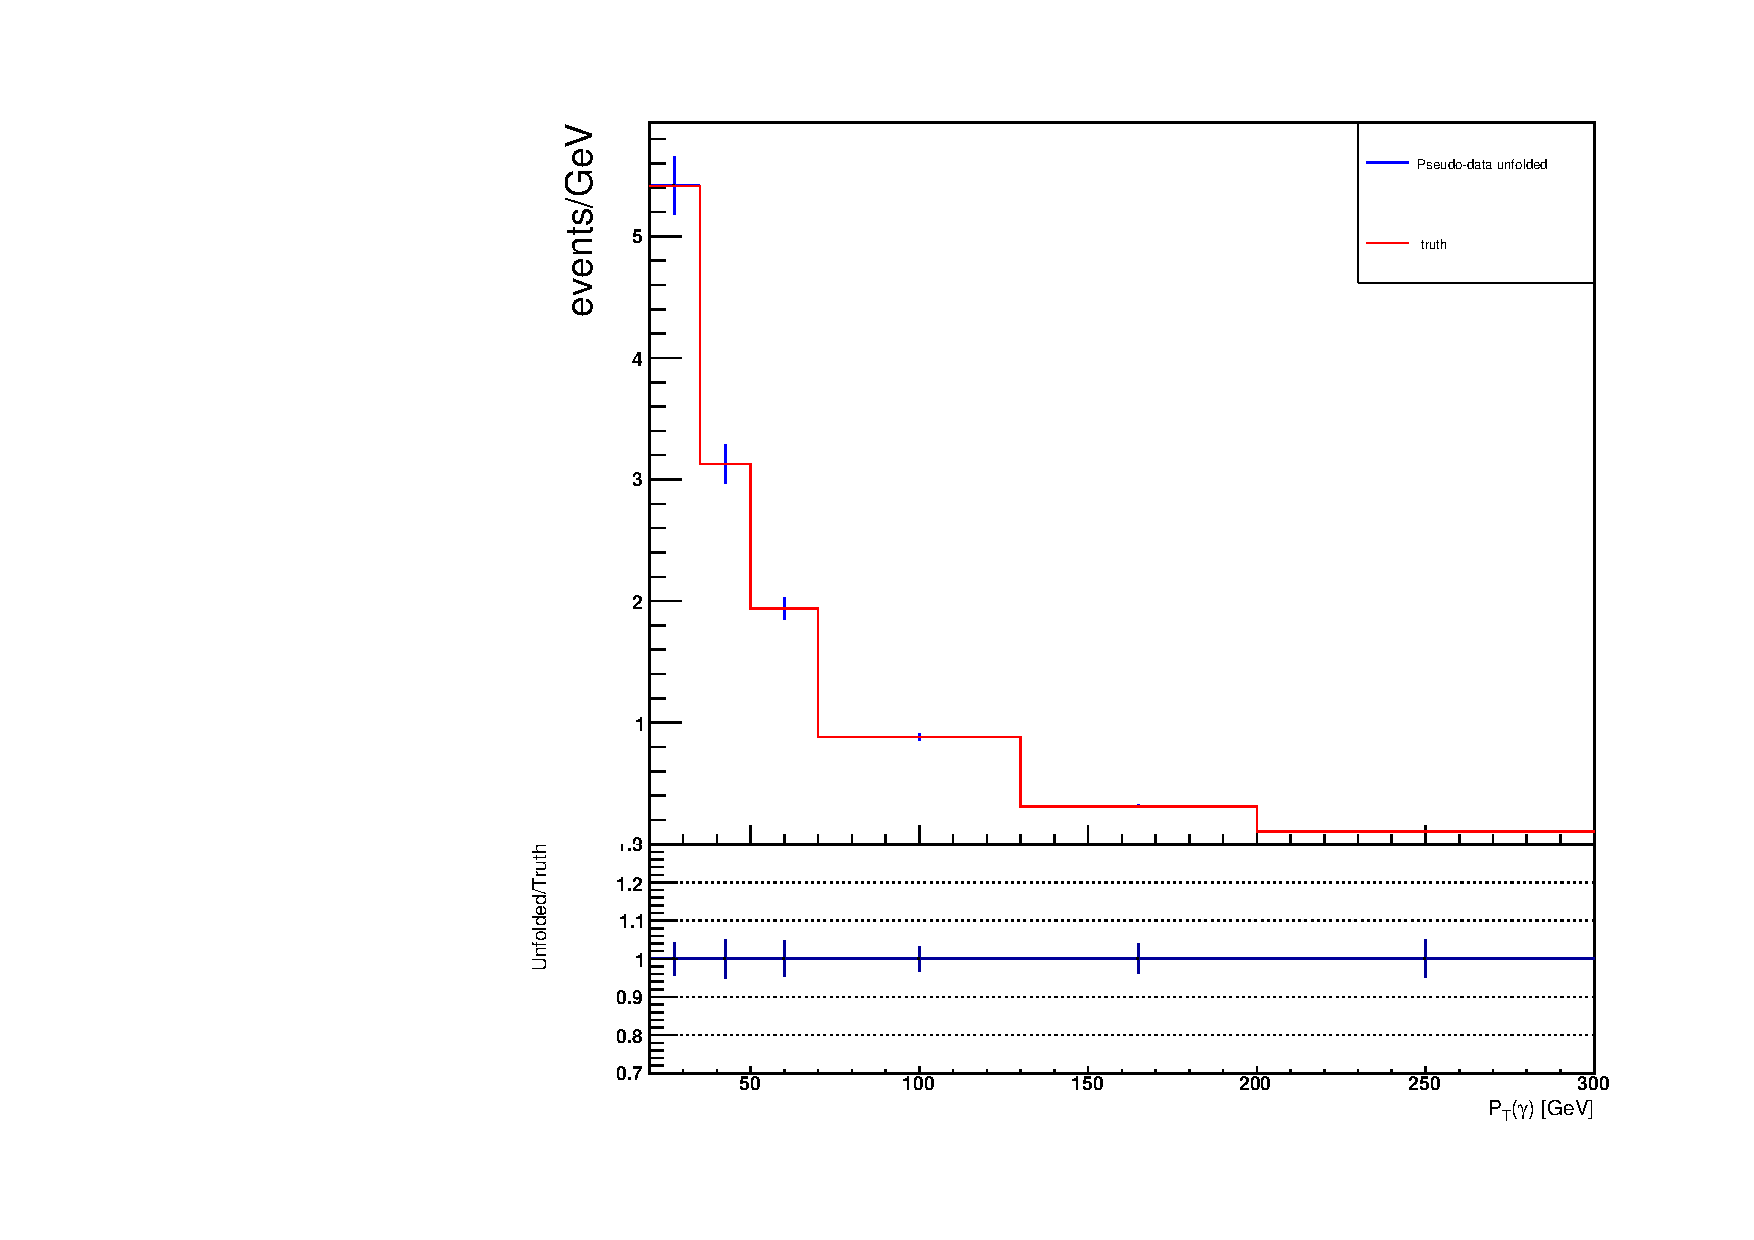
\includegraphics[width=0.4\textwidth]{figures/diff_xsec/ljet/Unfolding_tests/Closure_test/tty1l_pt_all_stat.pdf}}
  \quad\quad
  \subfloat[]{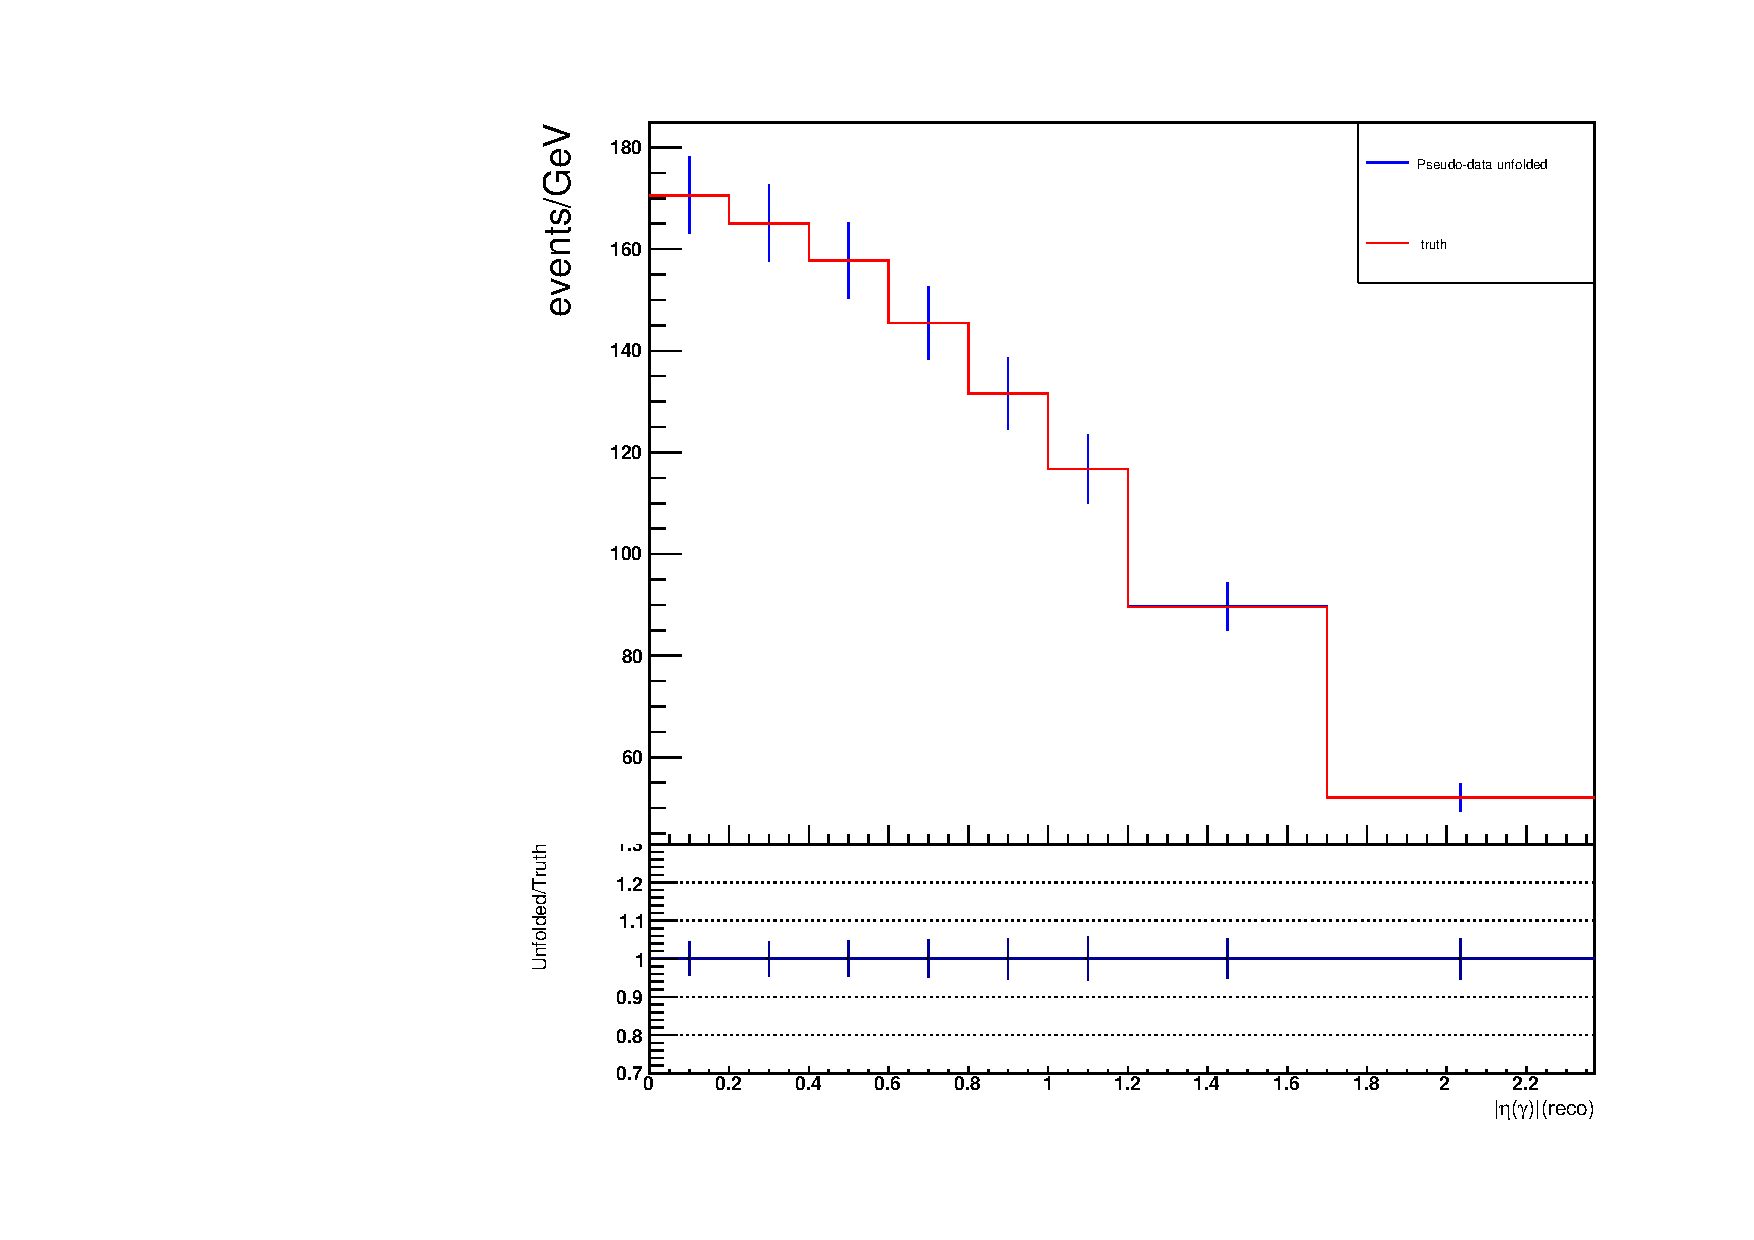
\includegraphics[width=0.4\textwidth]{figures/diff_xsec/ljet/Unfolding_tests/Closure_test/tty1l_eta_all_stat.pdf}}
  \quad\quad
  \subfloat[]{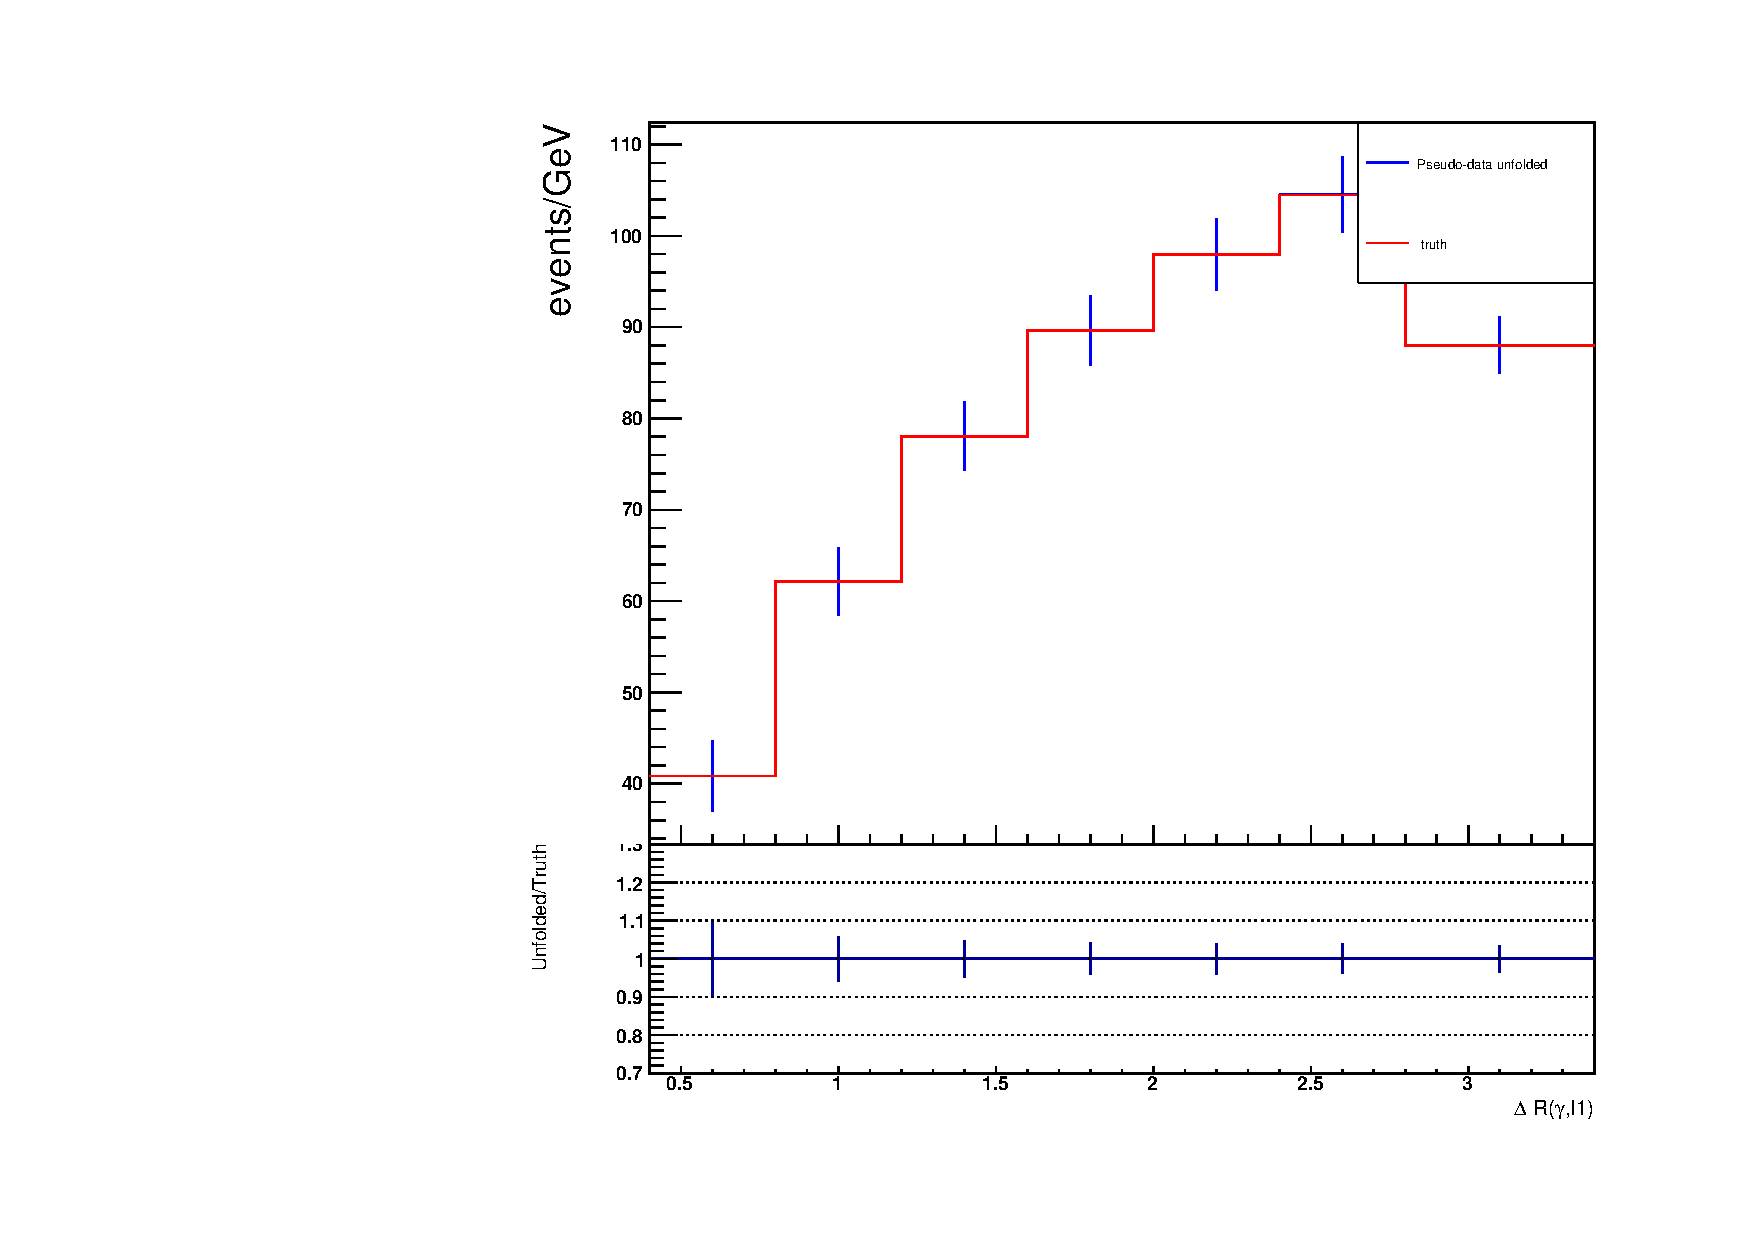
\includegraphics[width=0.4\textwidth]{figures/diff_xsec/ljet/Unfolding_tests/Closure_test/tty1l_dr_all_stat.pdf}}
  \quad\quad
  \subfloat[]{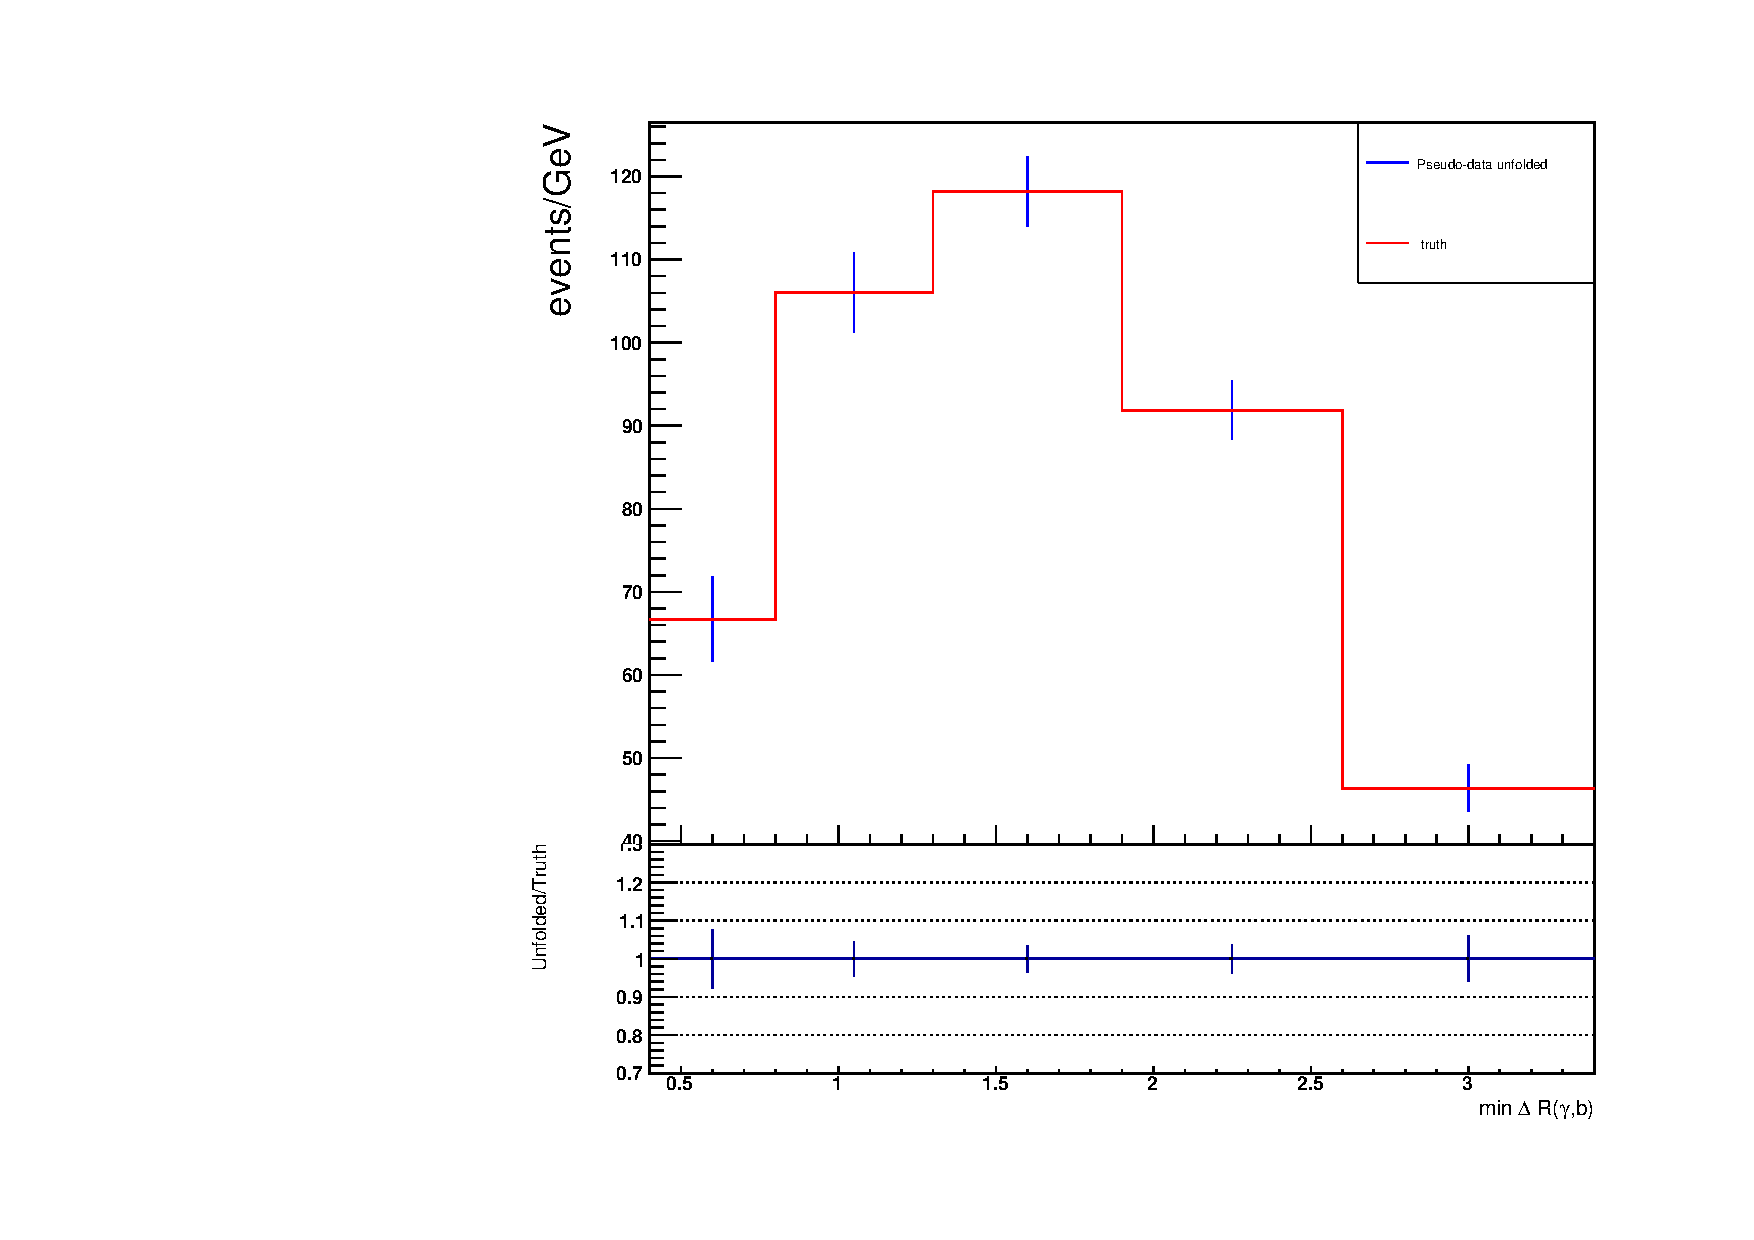
\includegraphics[width=0.4\textwidth]{figures/diff_xsec/ljet/Unfolding_tests/Closure_test/tty1l_drphb_all_stat.pdf}}
  \quad\quad
  \subfloat[]{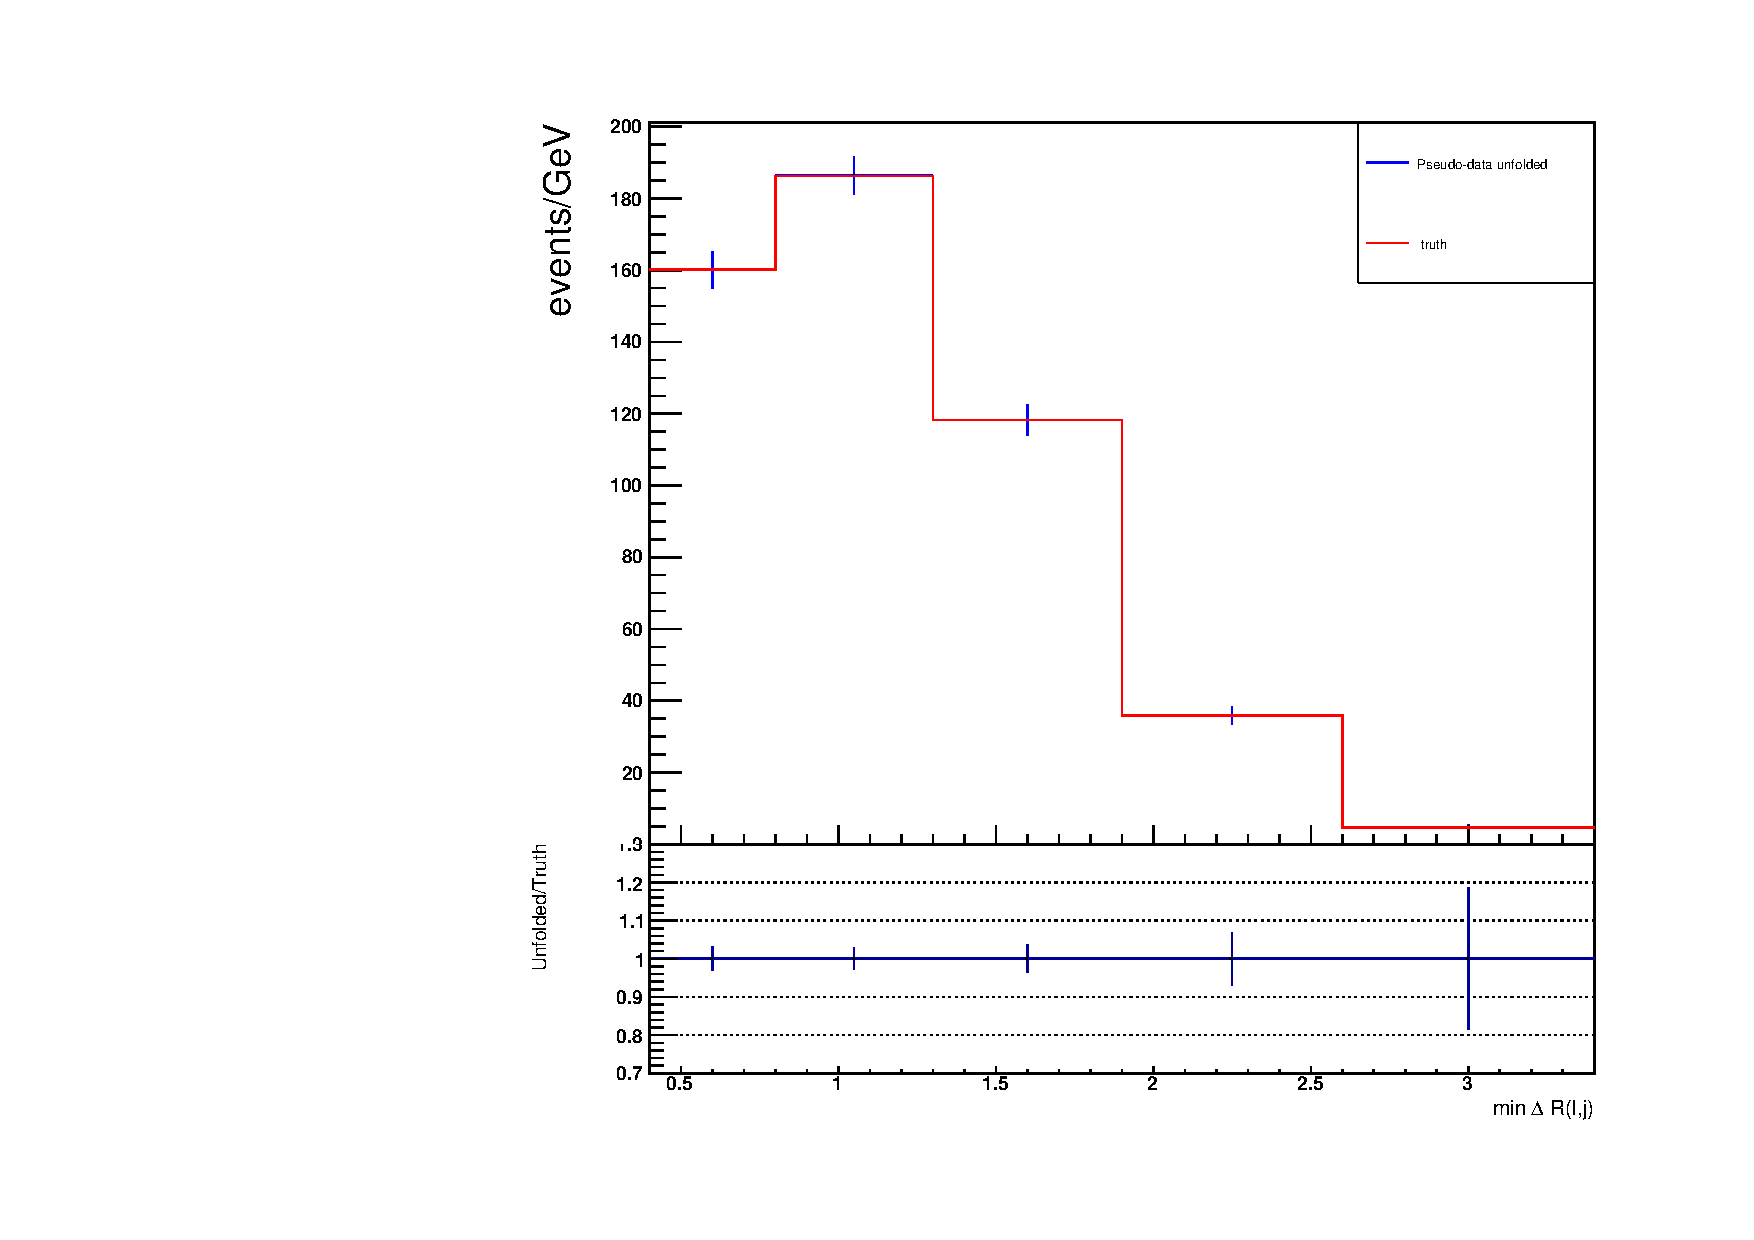
\includegraphics[width=0.4\textwidth]{figures/diff_xsec/ljet/Unfolding_tests/Closure_test/tty1l_drlj_all_stat.pdf}}
  \quad\quad
  \subfloat[]{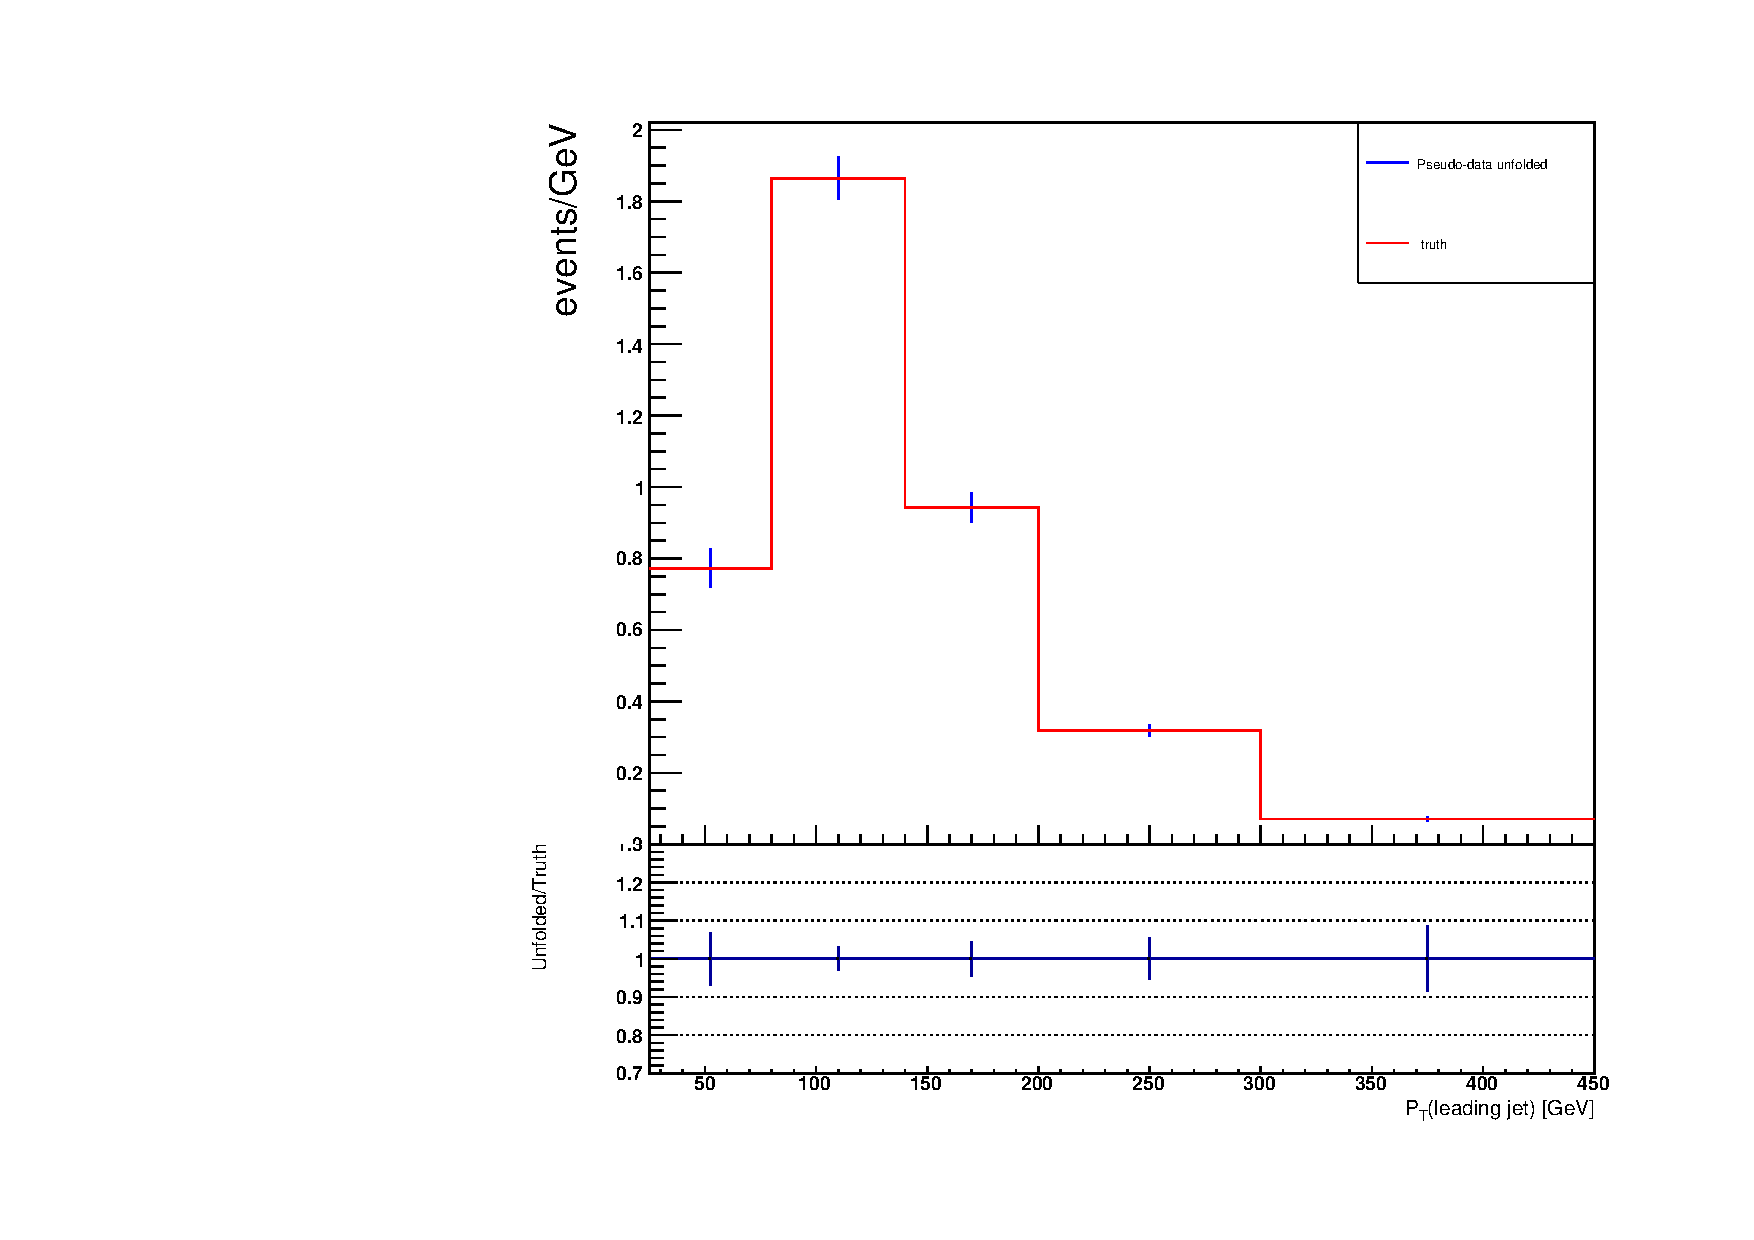
\includegraphics[width=0.4\textwidth]{figures/diff_xsec/ljet/Unfolding_tests/Closure_test/tty1l_ptj1_all_stat.pdf}}
  \quad\quad
  \caption{Comparison of the unfolded pseudo-data and the true distribution as a function of various observables. The uncertainty bars displayed in the plots represent only the statistical error considered in the unfolding. The above plots are specific to the single lepton channel.}
  \label{fig:unfolded_ljet_dist_closure}
\end{figure}
\FloatBarrier


\begin{figure}[ht]
  \centering
  \subfloat[]{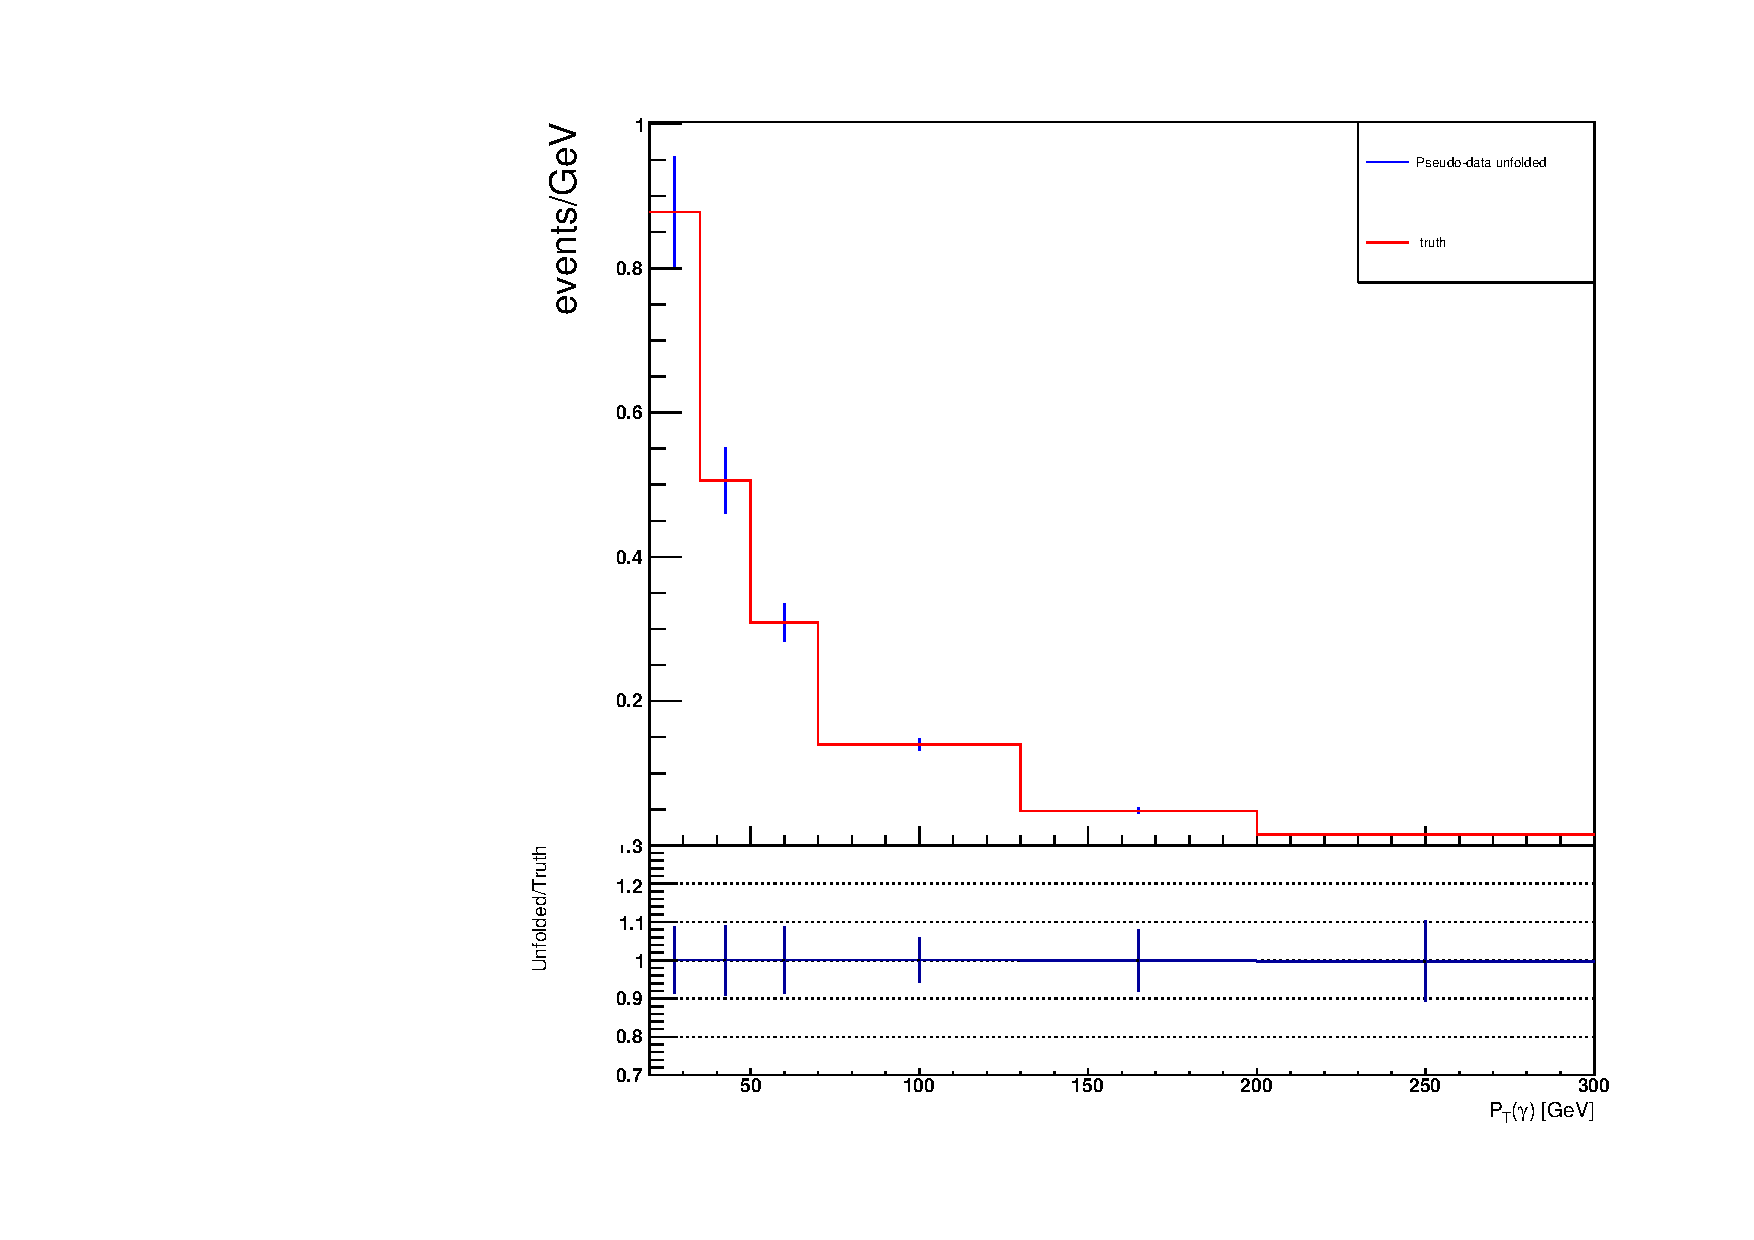
\includegraphics[width=0.4\textwidth]{figures/diff_xsec/dilep/Unfolding_tests/Closure_test/tty2l_pt_all_stat.pdf}}
  \quad\quad
  \subfloat[]{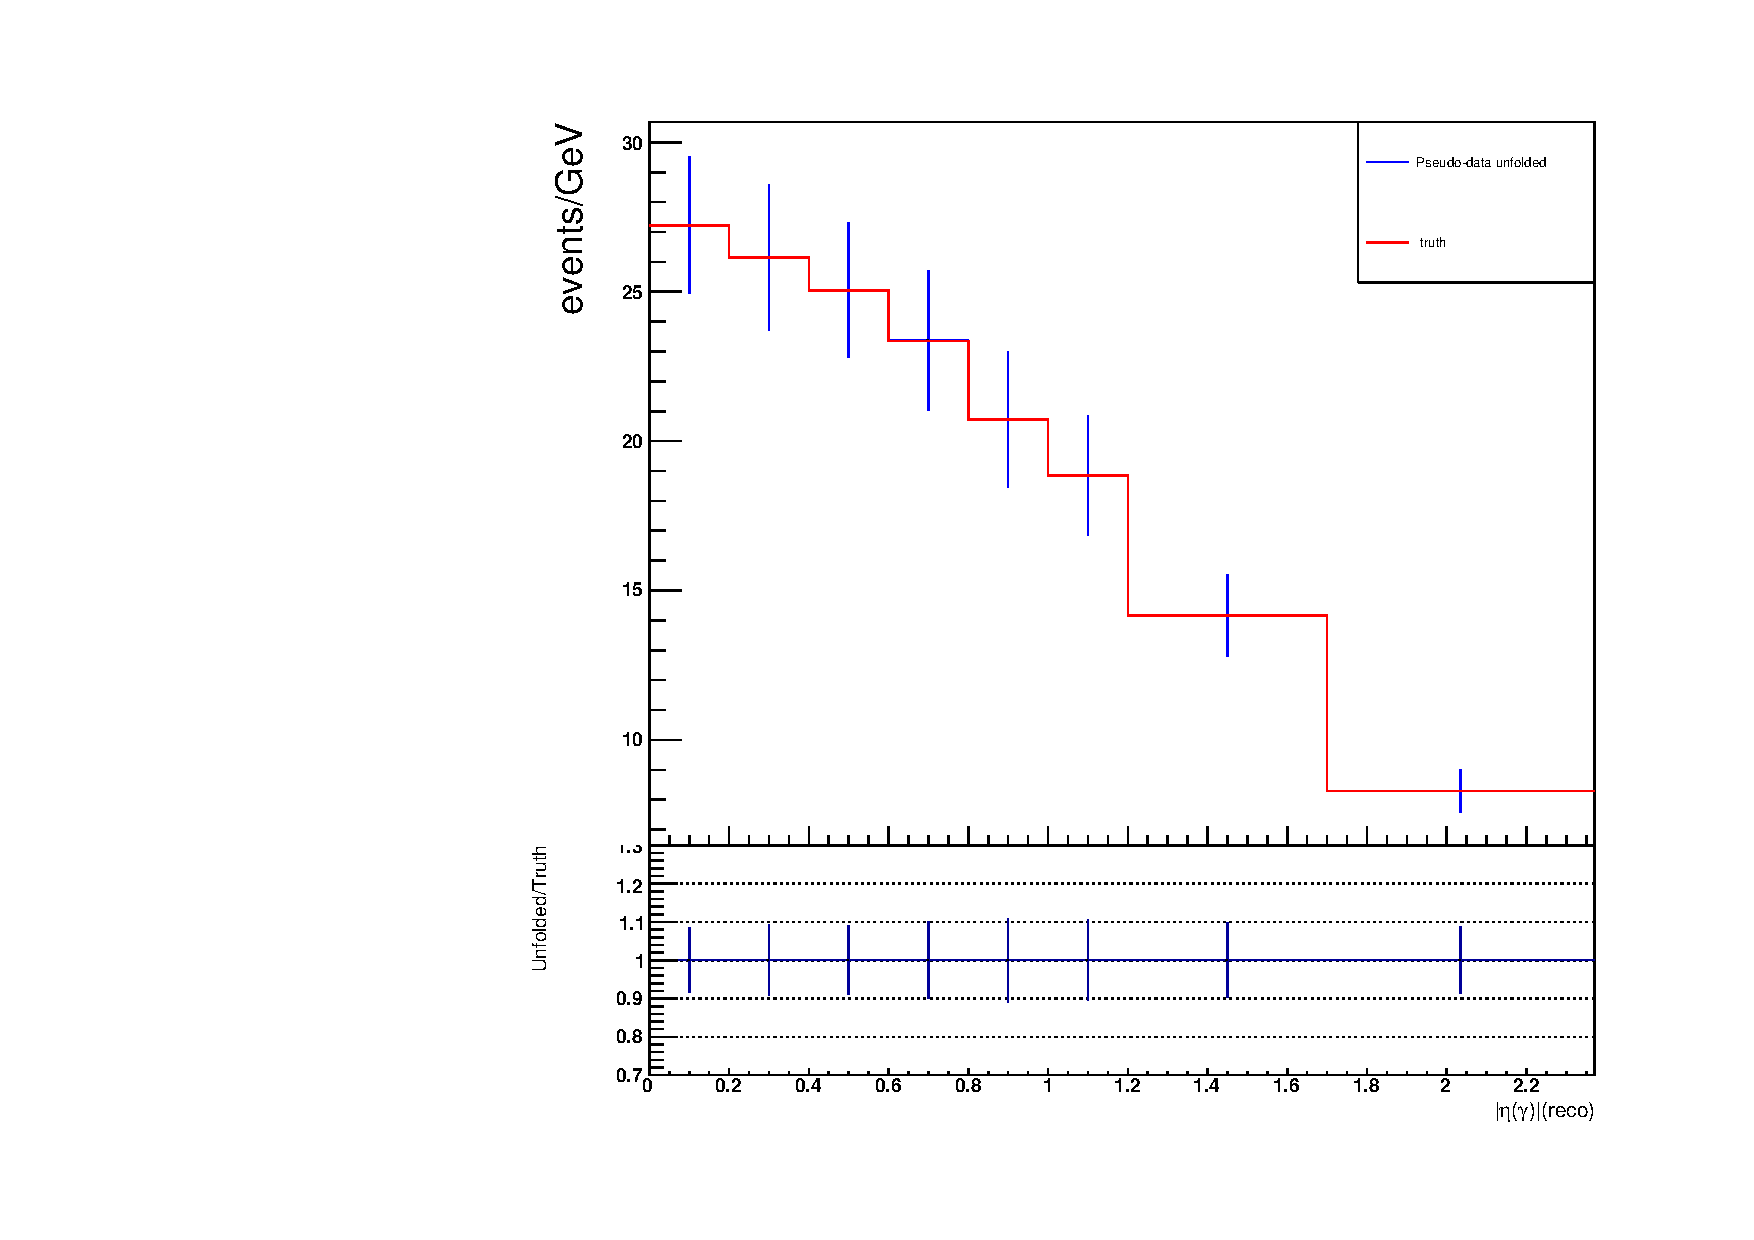
\includegraphics[width=0.4\textwidth]{figures/diff_xsec/dilep/Unfolding_tests/Closure_test/tty2l_eta_all_stat.pdf}}
  \quad\quad
  \subfloat[]{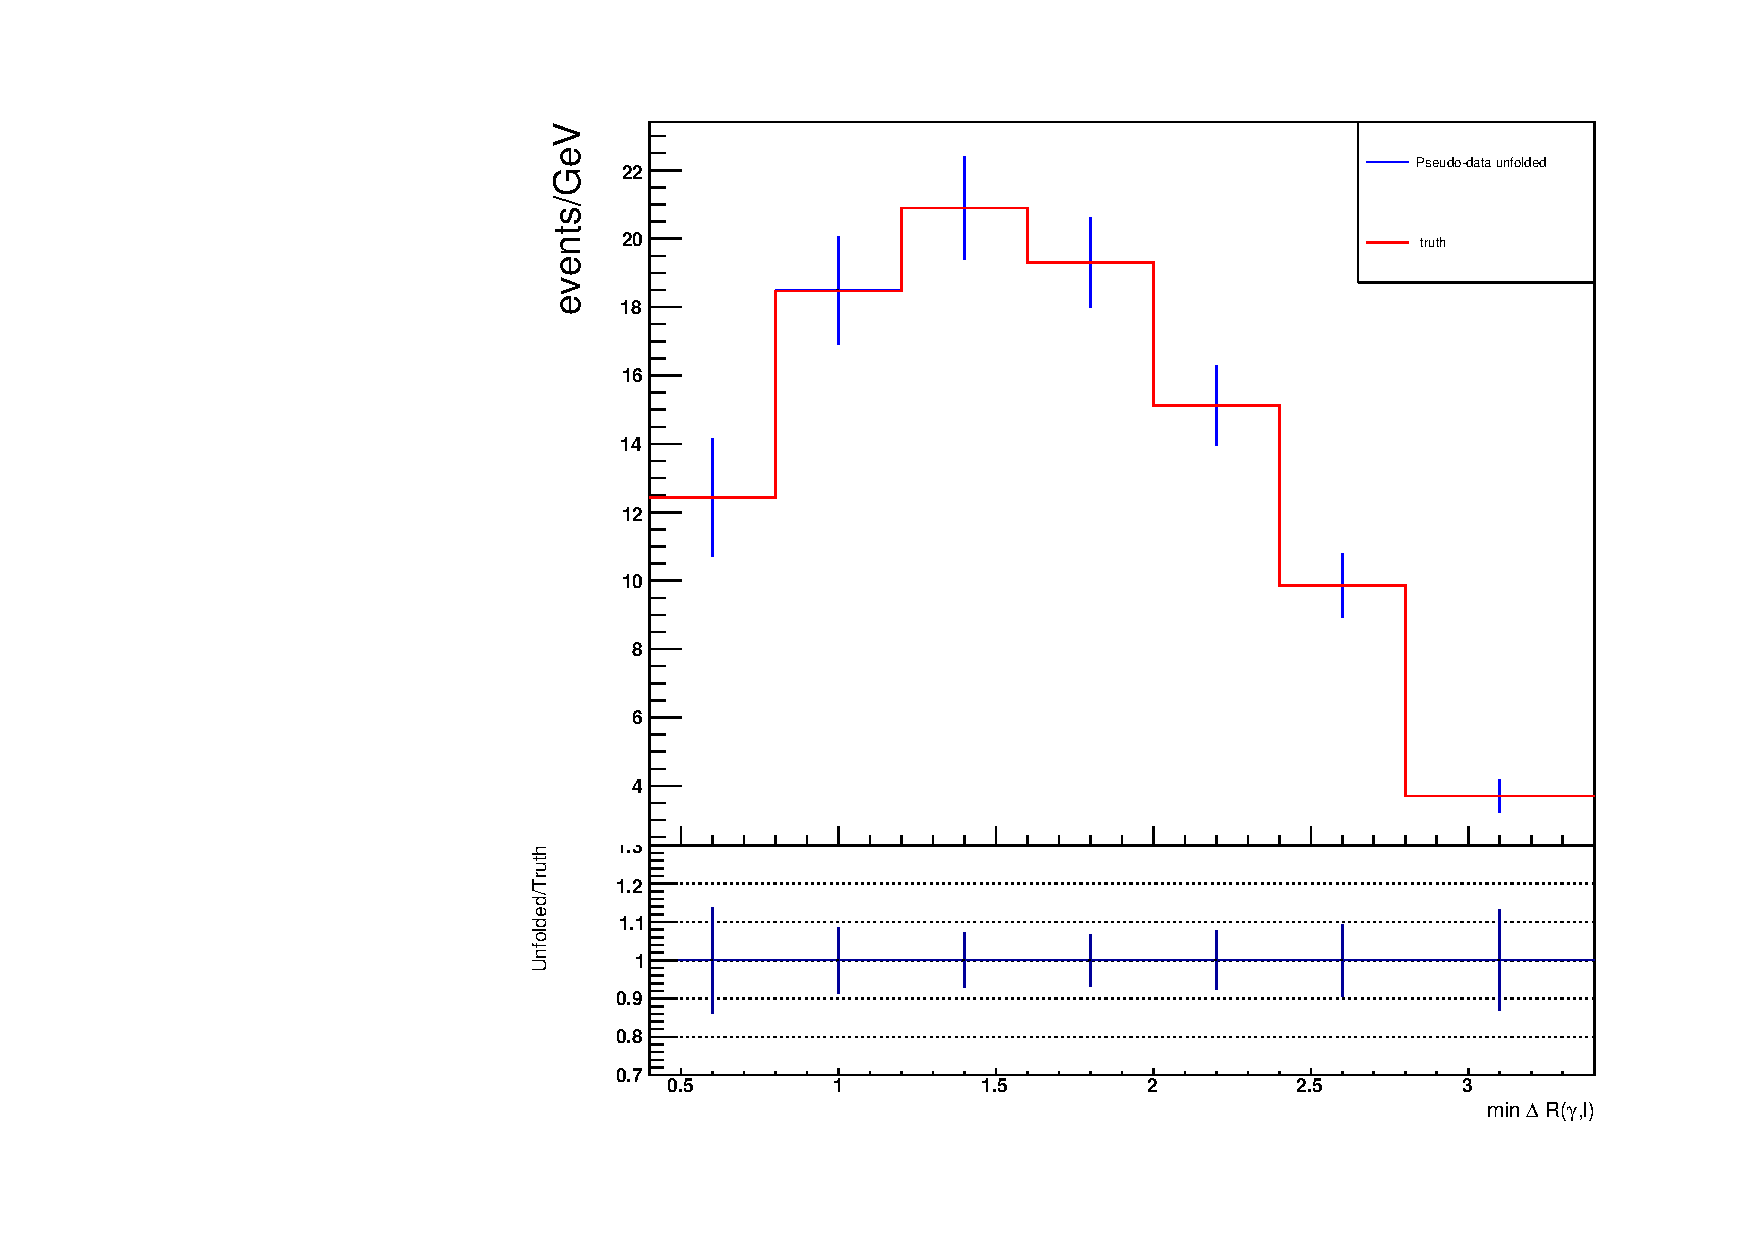
\includegraphics[width=0.4\textwidth]{figures/diff_xsec/dilep/Unfolding_tests/Closure_test/tty2l_dr_all_stat.pdf}}
  \quad\quad
  \subfloat[]{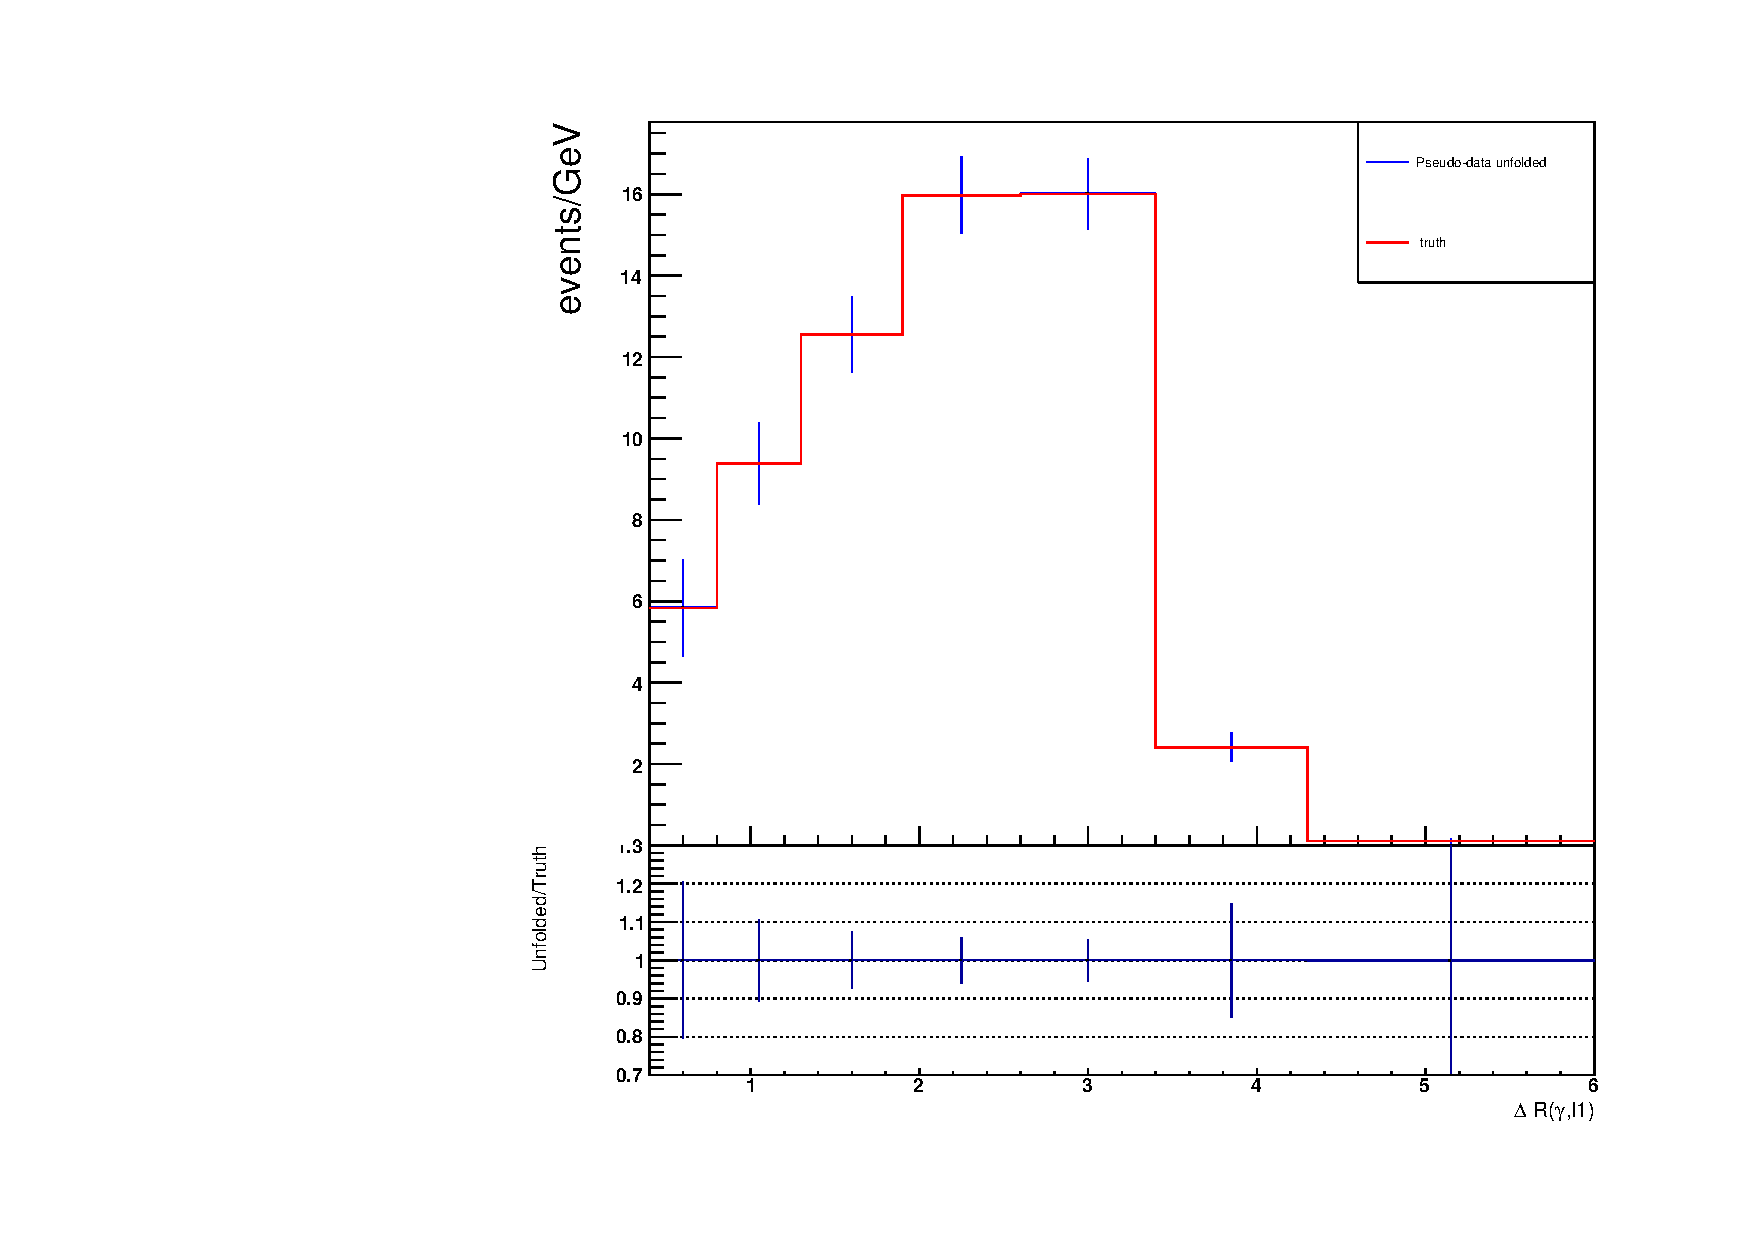
\includegraphics[width=0.4\textwidth]{figures/diff_xsec/dilep/Unfolding_tests/Closure_test/tty2l_dr1_all_stat.pdf}}
  \quad\quad
  \subfloat[]{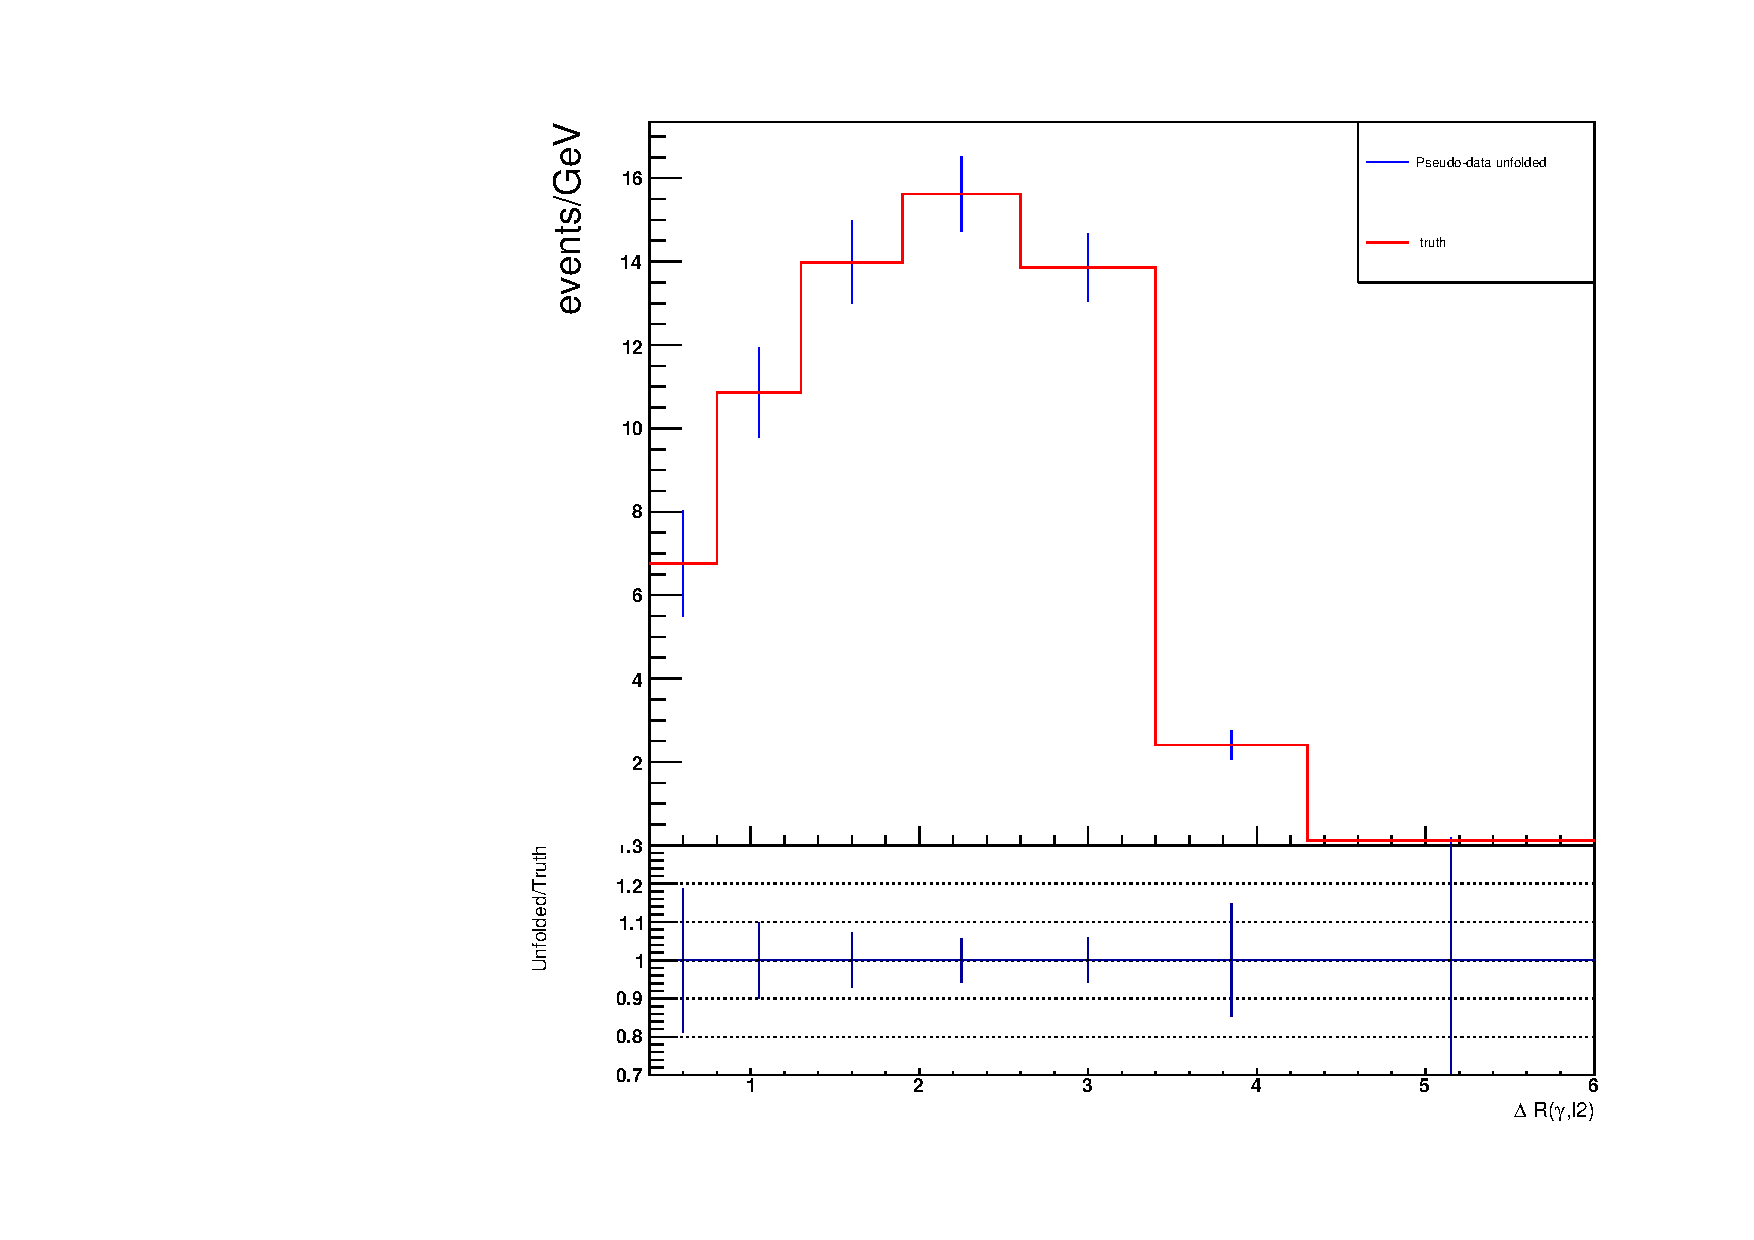
\includegraphics[width=0.4\textwidth]{figures/diff_xsec/dilep/Unfolding_tests/Closure_test/tty2l_dr2_all_stat.pdf}}
  \quad\quad
  \subfloat[]{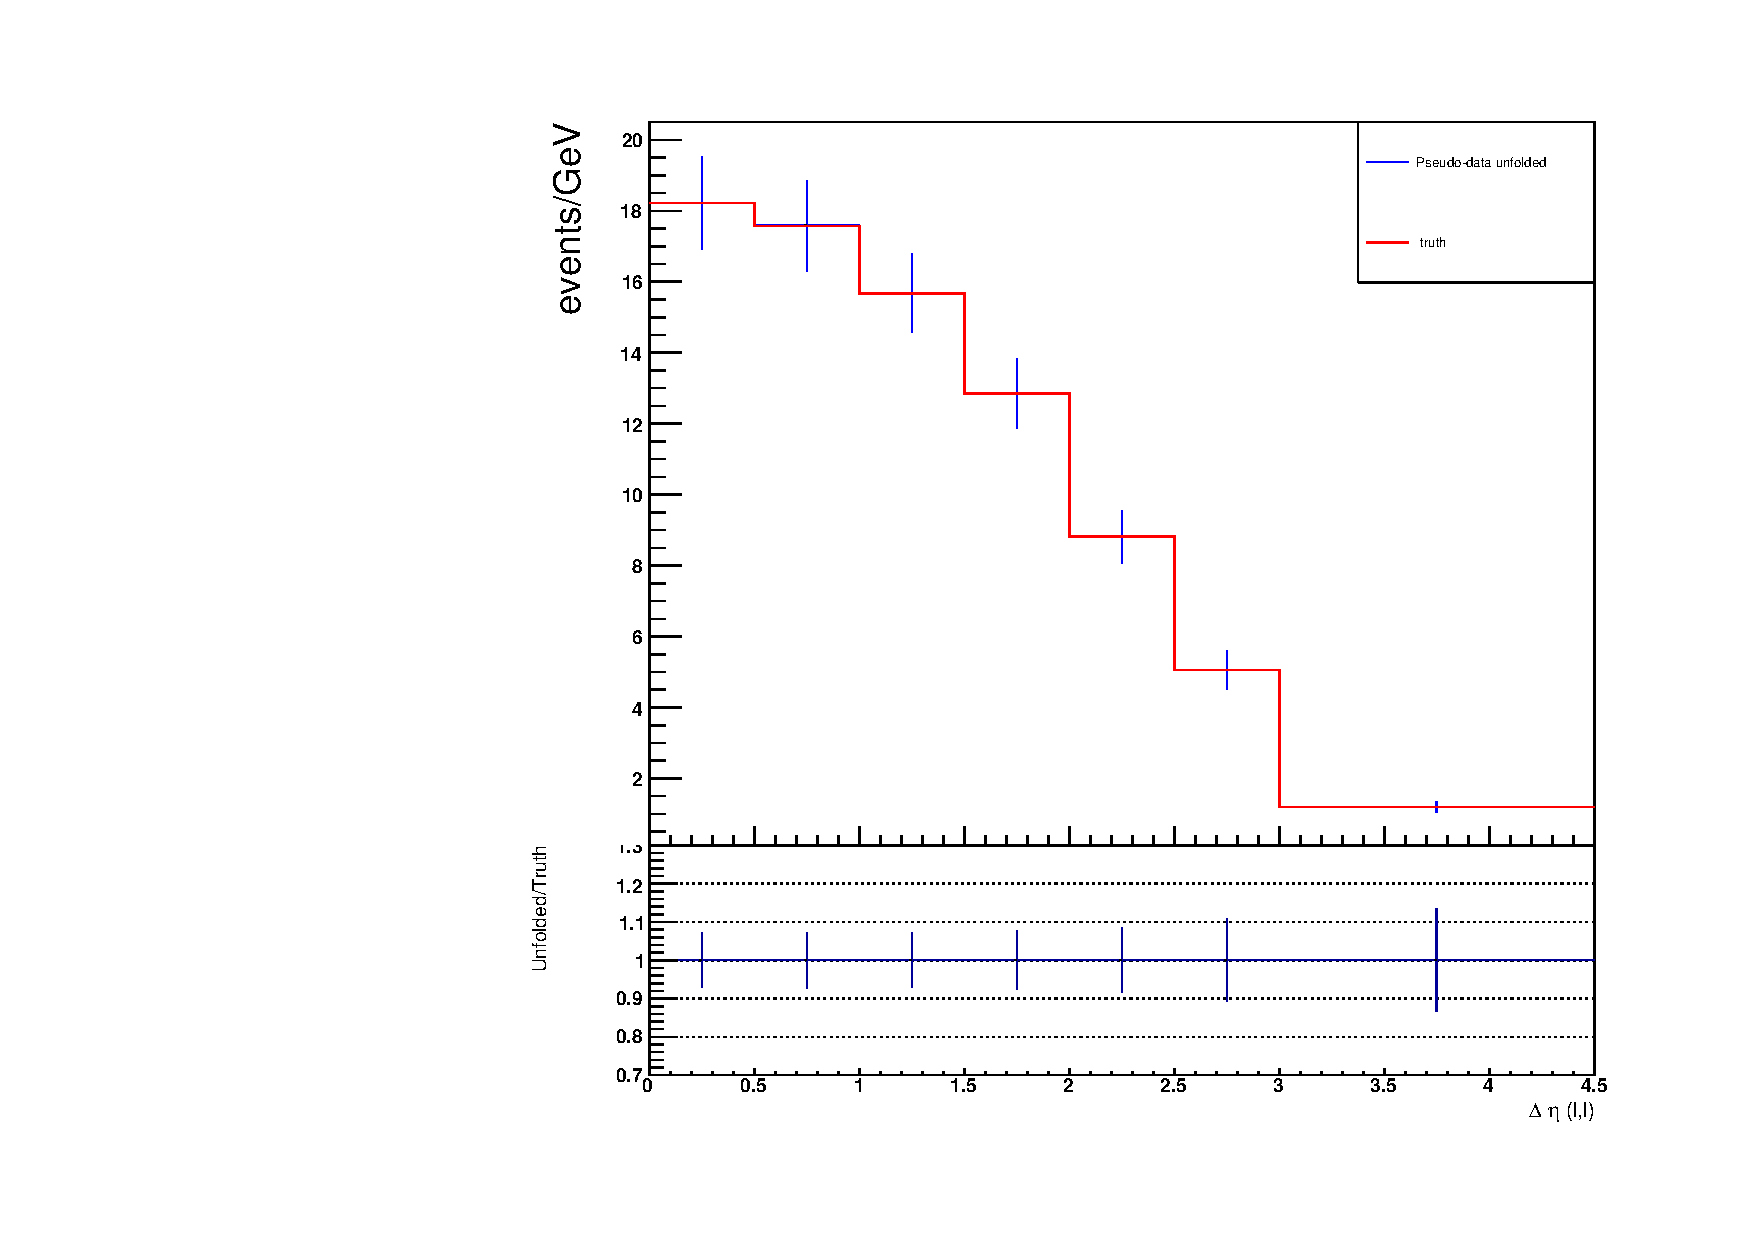
\includegraphics[width=0.4\textwidth]{figures/diff_xsec/dilep/Unfolding_tests/Closure_test/tty2l_dEtall_all_stat.pdf}}
  \caption{Comparison of the unfolded pseudo-data and the true distribution as a function of various observables. The uncertainty bars displayed in the plots represent only the statistical error considered in the unfolding. The above plots are specific to the dilepton channel.}
  \label{fig:unfolded_dilep_dist_closure_1}
\end{figure}

\begin{figure}[ht]
  \centering
  \subfloat[]{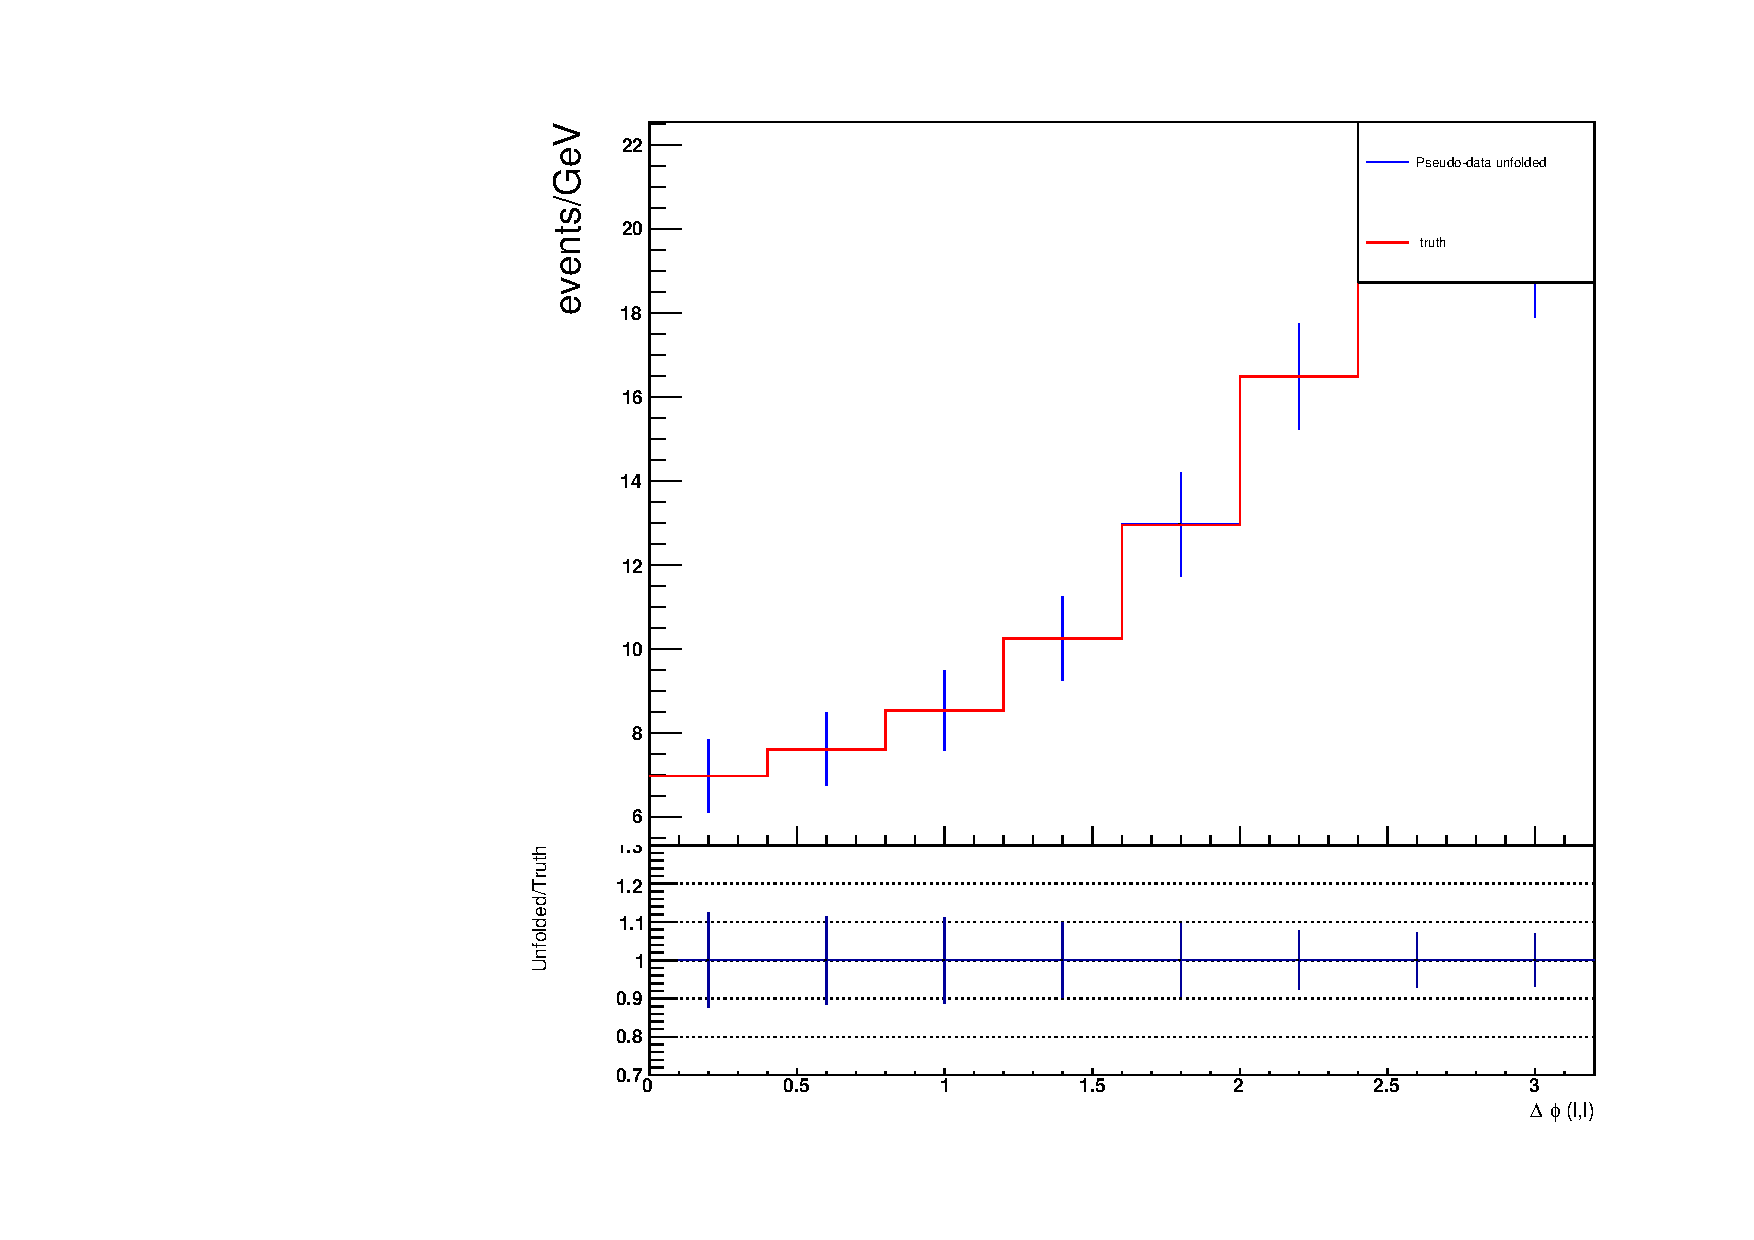
\includegraphics[width=0.4\textwidth]{figures/diff_xsec/dilep/Unfolding_tests/Closure_test/tty2l_dPhill_all_stat.pdf}}
  \quad\quad
  \subfloat[]{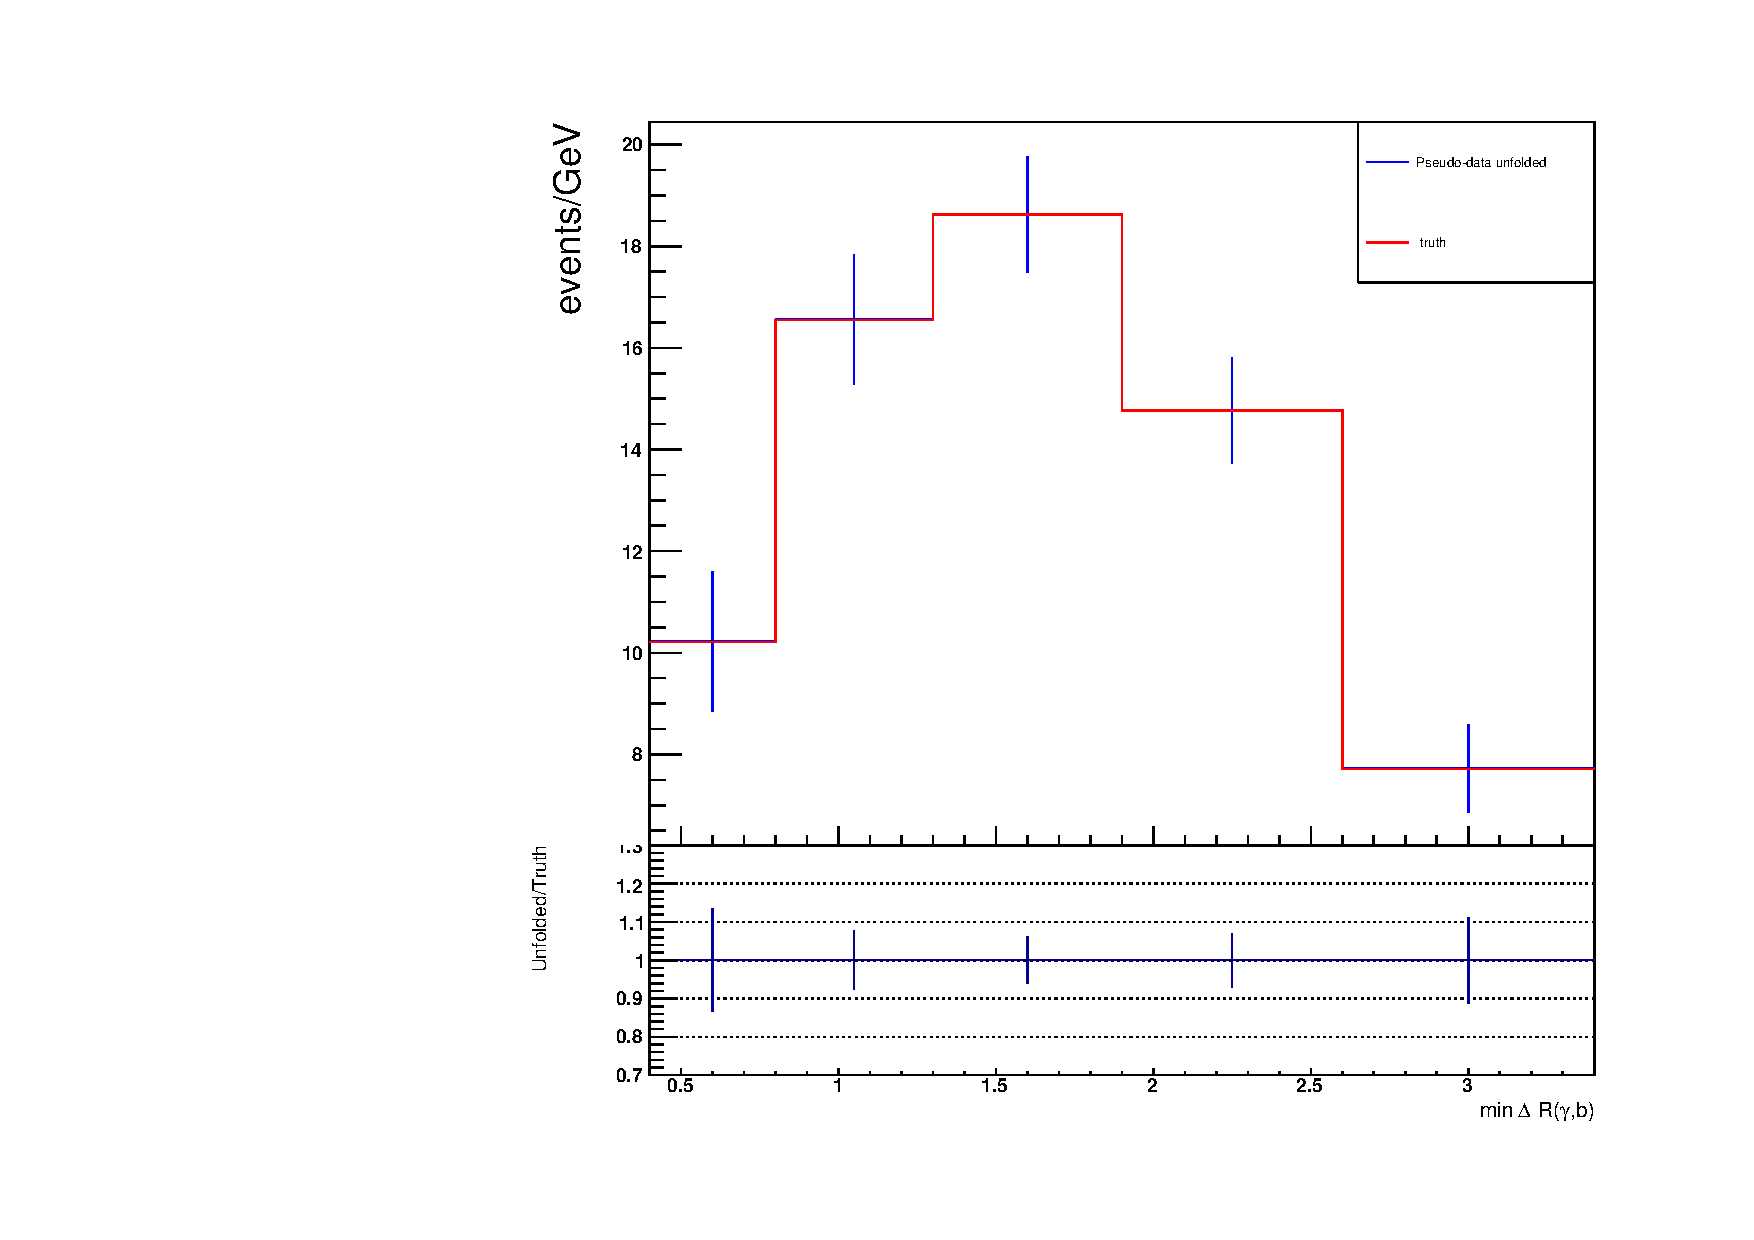
\includegraphics[width=0.4\textwidth]{figures/diff_xsec/dilep/Unfolding_tests/Closure_test/tty2l_drphb_all_stat.pdf}}
  \quad\quad
  \subfloat[]{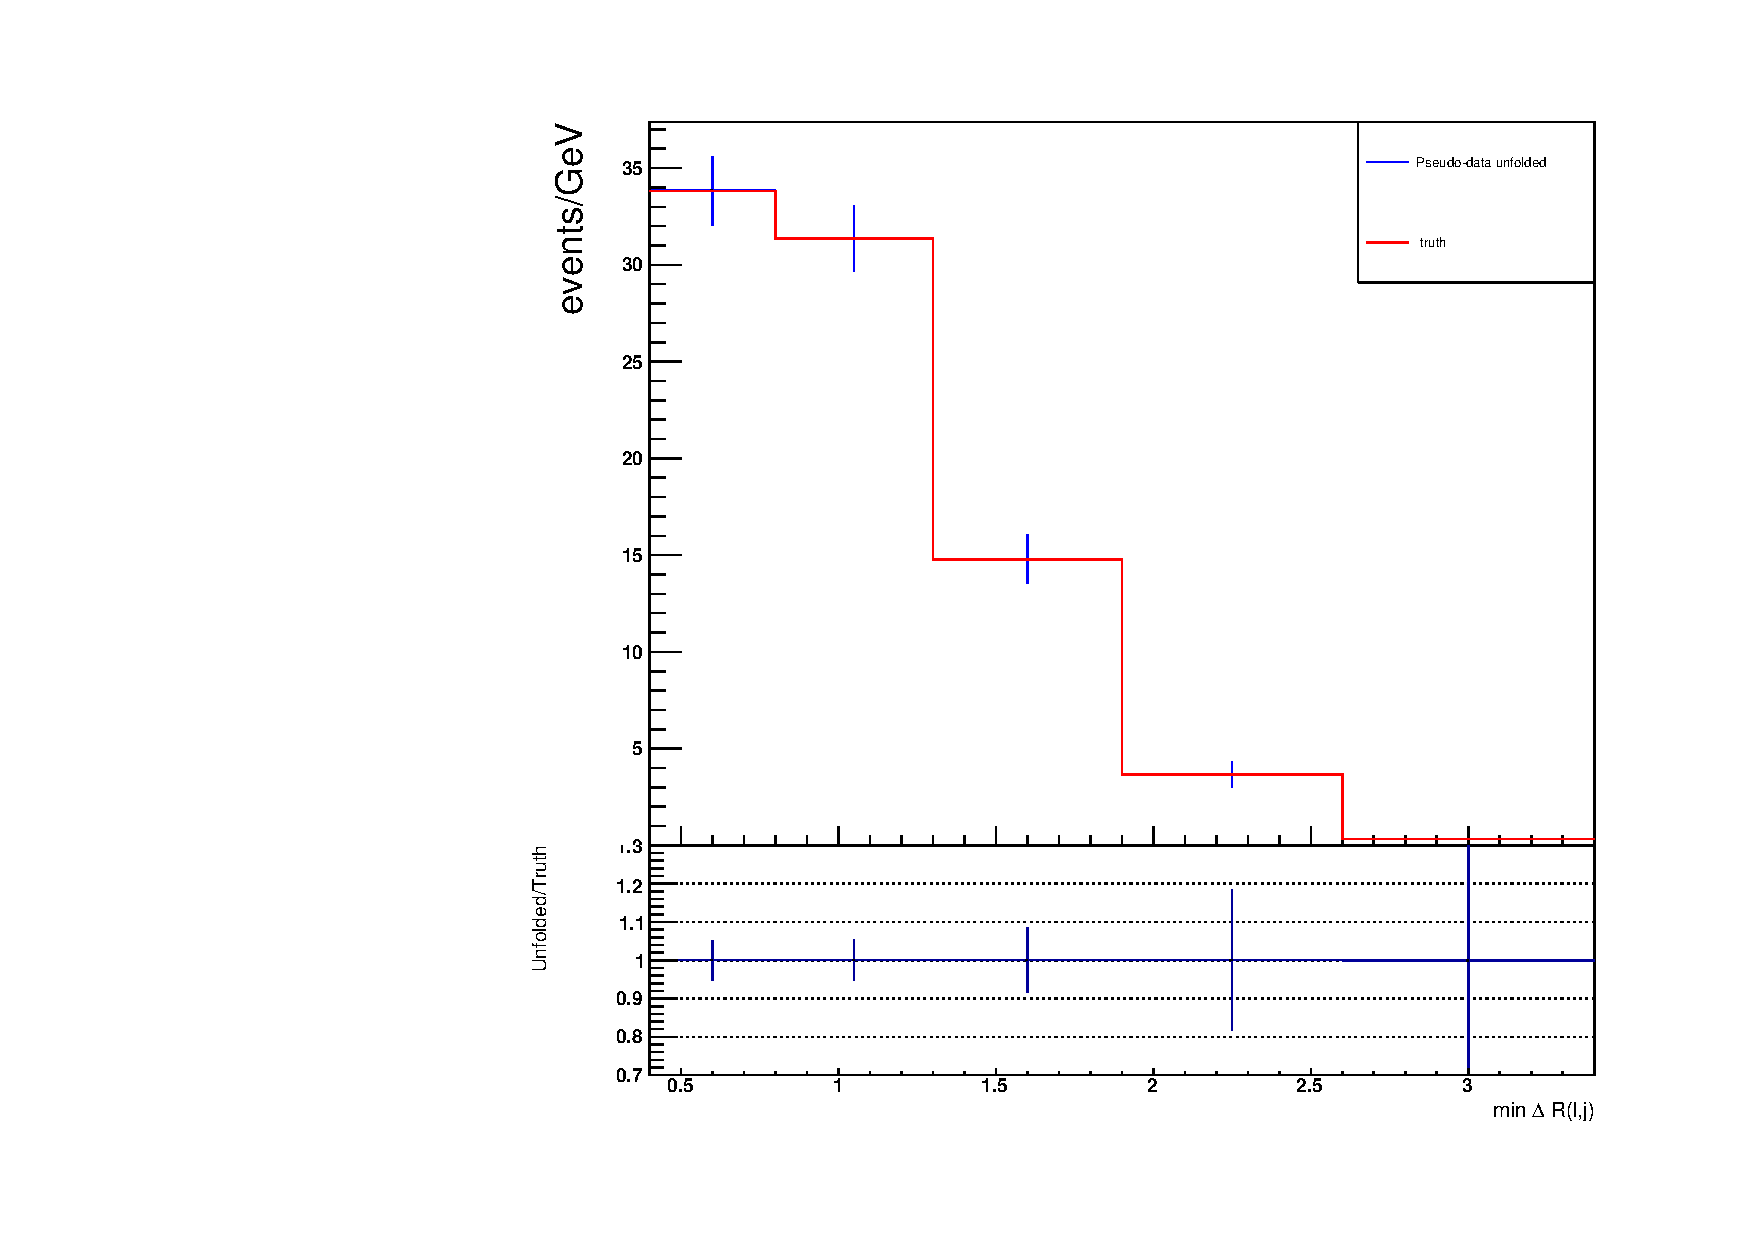
\includegraphics[width=0.4\textwidth]{figures/diff_xsec/dilep/Unfolding_tests/Closure_test/tty2l_drlj_all_stat.pdf}}
  \quad\quad
  \subfloat[]{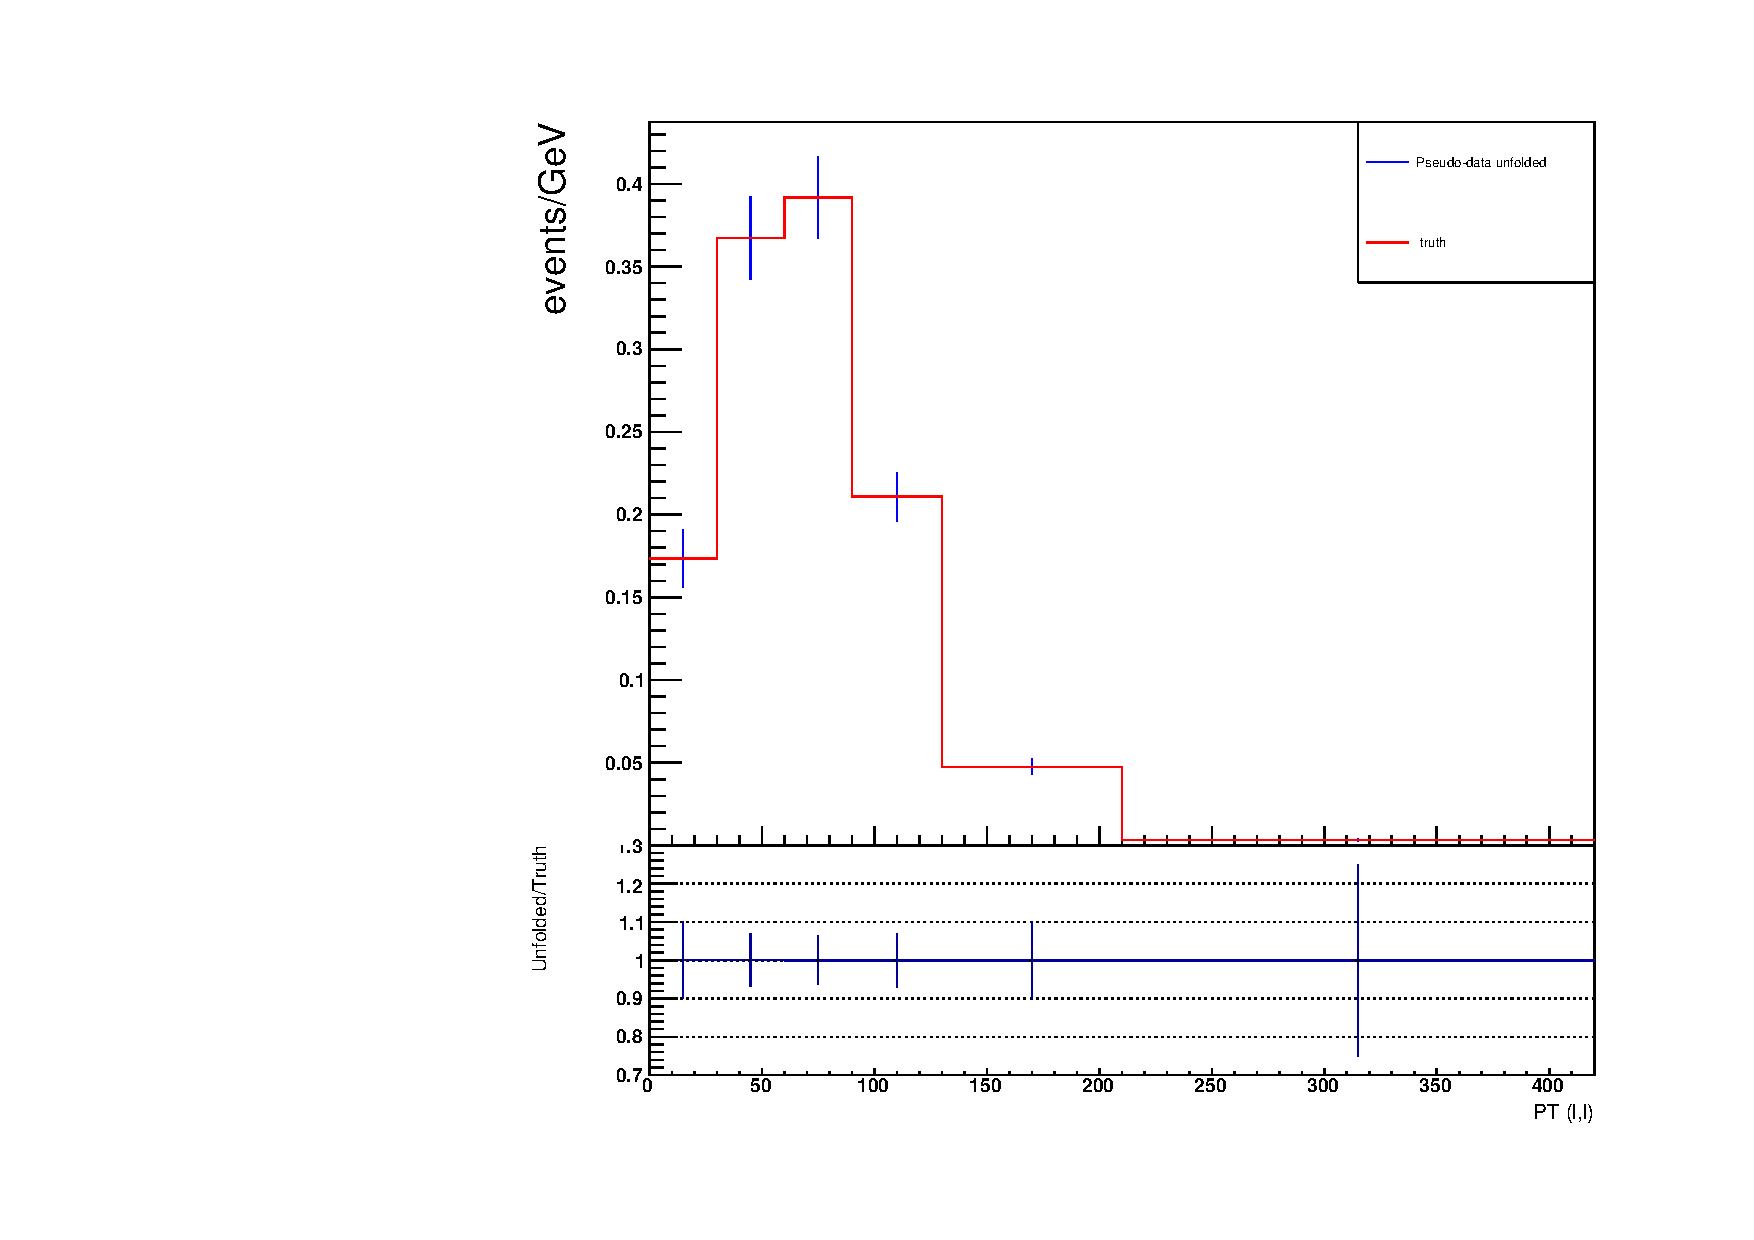
\includegraphics[width=0.4\textwidth]{figures/diff_xsec/dilep/Unfolding_tests/Closure_test/tty2l_ptll_all_stat.pdf}}
  \quad\quad
  \subfloat[]{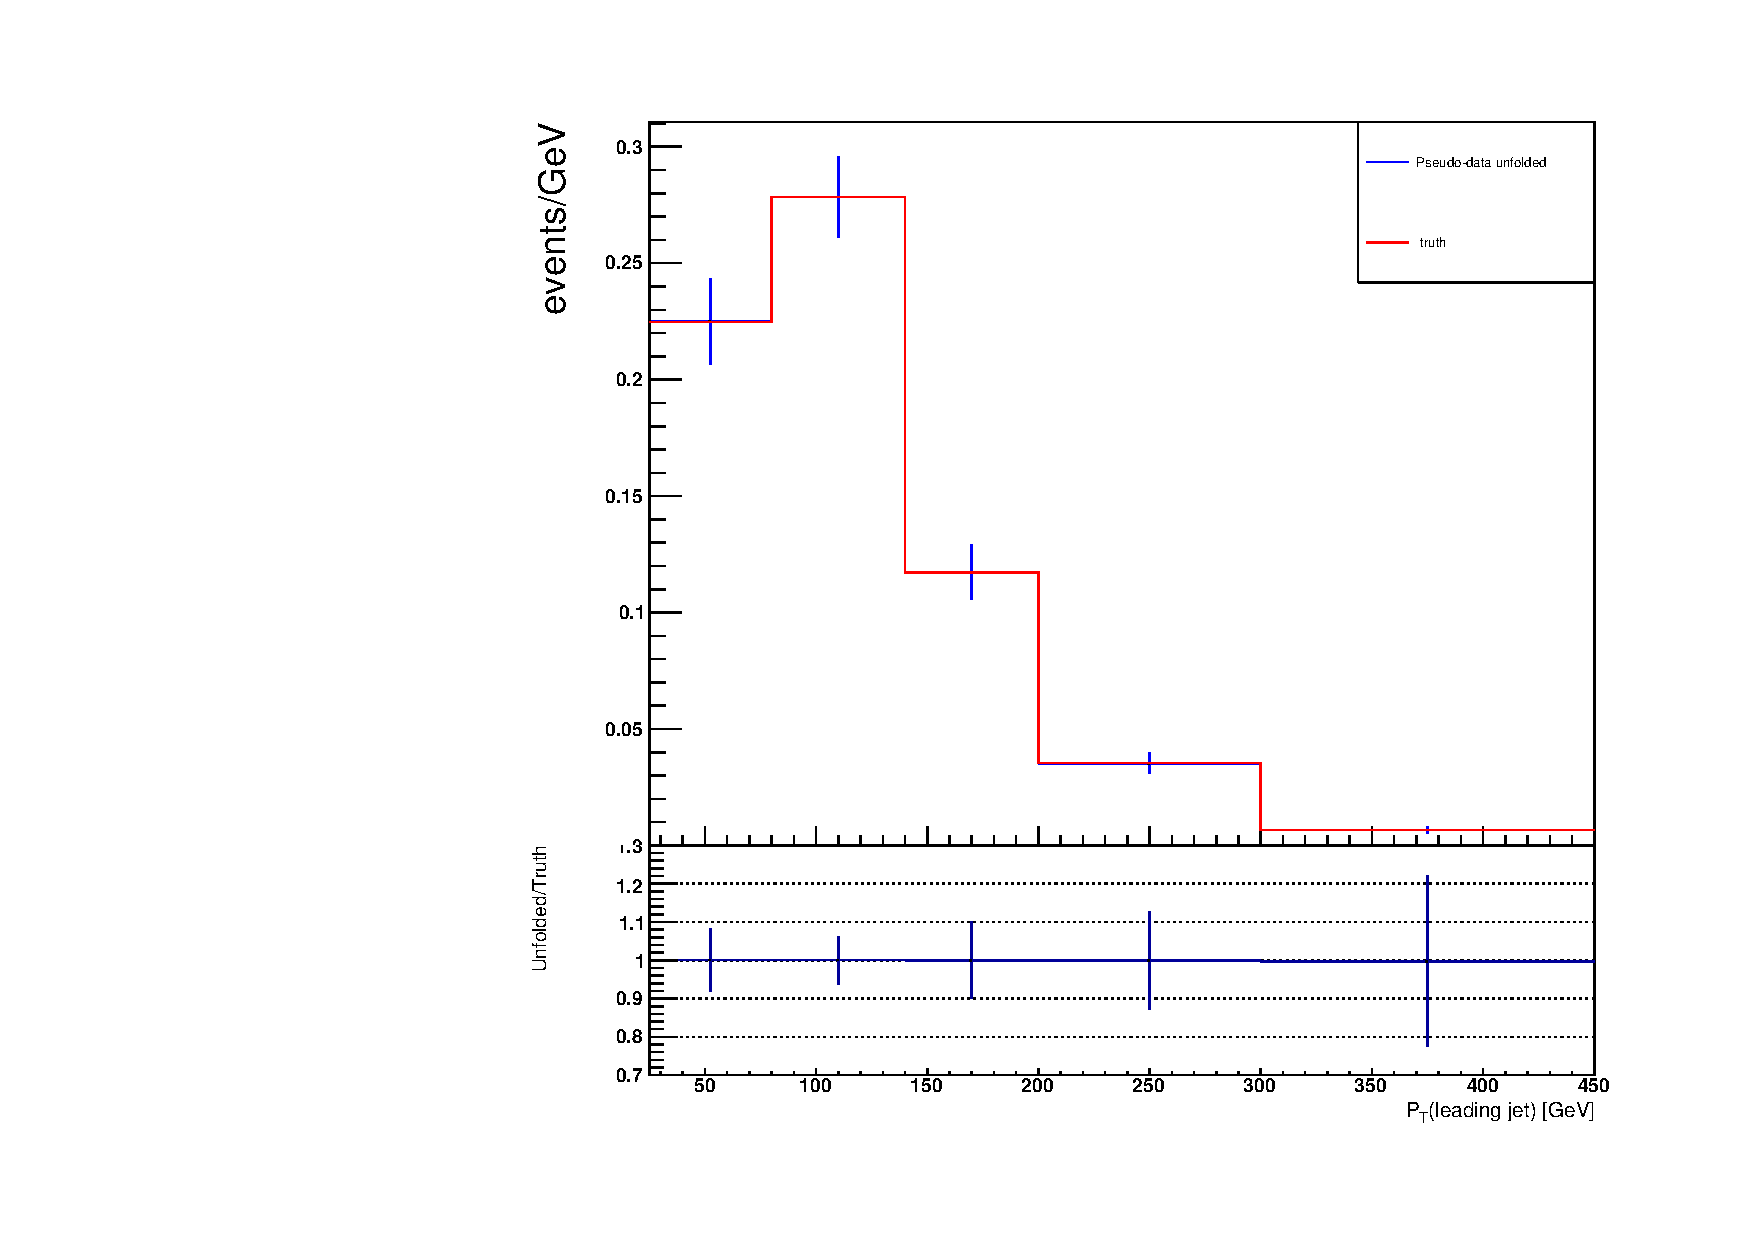
\includegraphics[width=0.4\textwidth]{figures/diff_xsec/dilep/Unfolding_tests/Closure_test/tty2l_ptj1_all_stat.pdf}}
  \quad\quad
  \caption{Comparison of the unfolded pseudo-data and the true distribution 
  as a function of various observables. The uncertainty bars displayed in the plots represent only 
  the statistical error considered in the unfolding. The above plots are specific to the dilepton channel.}
  \label{fig:unfolded_dilep_dist_closure_2}
\end{figure}
\FloatBarrier




\subsection{Stress Test}
\label{sec:stress_test}
The stress test is performed in order to verify that the unfolding procedure is not biased to any specific shape of the particle level distribution. The particle-level and reconstruction-level distributions obtained from the nominal MC sample are reweighed, and then the reweighted reconstructed distribution is unfolded using the nominal inputs from the MC sample, and the unfolded results are compared to the corresponding particle level distribution. Different weights have been checked, the first one is by taking the observed difference at reconstruction level between data and MC as the following:

$$ \mathrm{weight} = 1 + \mathrm{Y} \times \frac{\mathrm{data}_i - \mathrm{MC}_i}{\mathrm{data}_i} = 1 + Y \times \mathrm{Obs}, $$
where $i$ is the bin index and Y = 1, -1. The result of the stress test is shown in Figure ~\ref{fig:unfolded_ljet_dist_stress_test}for single lepton channel and in Figure ~\ref{fig:unfolded_dilep_dist_stress_test_1},Figure ~\ref{fig:unfolded_dilep_dist_stress_test_2} for dilepton channel. The unfolding is able to retrieve the reweighted particle distribution for all observables in both channels. \\

A different weight, corresponding to a linear skewness of the shape, is used. It is defined as the following, in case of the $p_T$ distributions ($p_T(\gamma), p_T(j1), p_T(ll)$):

$$ \mathrm{weight} = 1 + \mathrm{Y} \times \frac{100 - i}{300} = 1 + \mathrm{Y} \times \mathrm{X}, $$
and for the photon $\eta$:
$$ \mathrm{weight} = 1 + \mathrm{Y} \times \frac{1.2 - i}{2.37} = 1 + \mathrm{Y} \times \mathrm{X}, $$
and for the $ \mathrm{min} \Delta R(\gamma, \mathrm{l})$, $\Delta R(\gamma, \mathrm{l1})$, 
$\Delta R(\gamma, \mathrm{l2})$,  $\mathrm{min} \Delta R(\gamma, b)$, $\Delta R(l, j)$ by:
$$ \mathrm{weight} = 1 + \mathrm{Y} \times \frac{1.8 - i}{6} = 1 + \mathrm{Y} \times \mathrm{X}, $$
and for the $ \Delta \eta (\mathrm{lepton},\mathrm{lepton}) $ by:
$$ \mathrm{weight} = 1 + \mathrm{Y} \times \frac{1.2 - i}{2.5} = 1 + \mathrm{Y} \times \mathrm{X}, $$
and for the $ \Delta \phi (\mathrm{lepton}, \mathrm{lepton}) $ by:
$$ \mathrm{weight} = 1 + \mathrm{Y} \times \frac{1.75 - i}{3.14} = 1 + \mathrm{Y} \times \mathrm{X}, $$

where Y = -1, 1, and $i$ is the bin centre. The results of the second stress test 
shown in the same Figure ~\ref{fig:unfolded_ljet_dist_stress_test} for 
single lepton channel and in Figures ~\ref{fig:unfolded_dilep_dist_stress_test_1}, 
~\ref{fig:unfolded_dilep_dist_stress_test_2} for dilepton channel. The reweighted particle level distributions are in different shapes from the nominal ones, and the unfolding procedure is able to retrieve the reweighted particle level distributions in all observables in both channels.


\begin{figure}[ht]
  \centering
  \subfloat[]{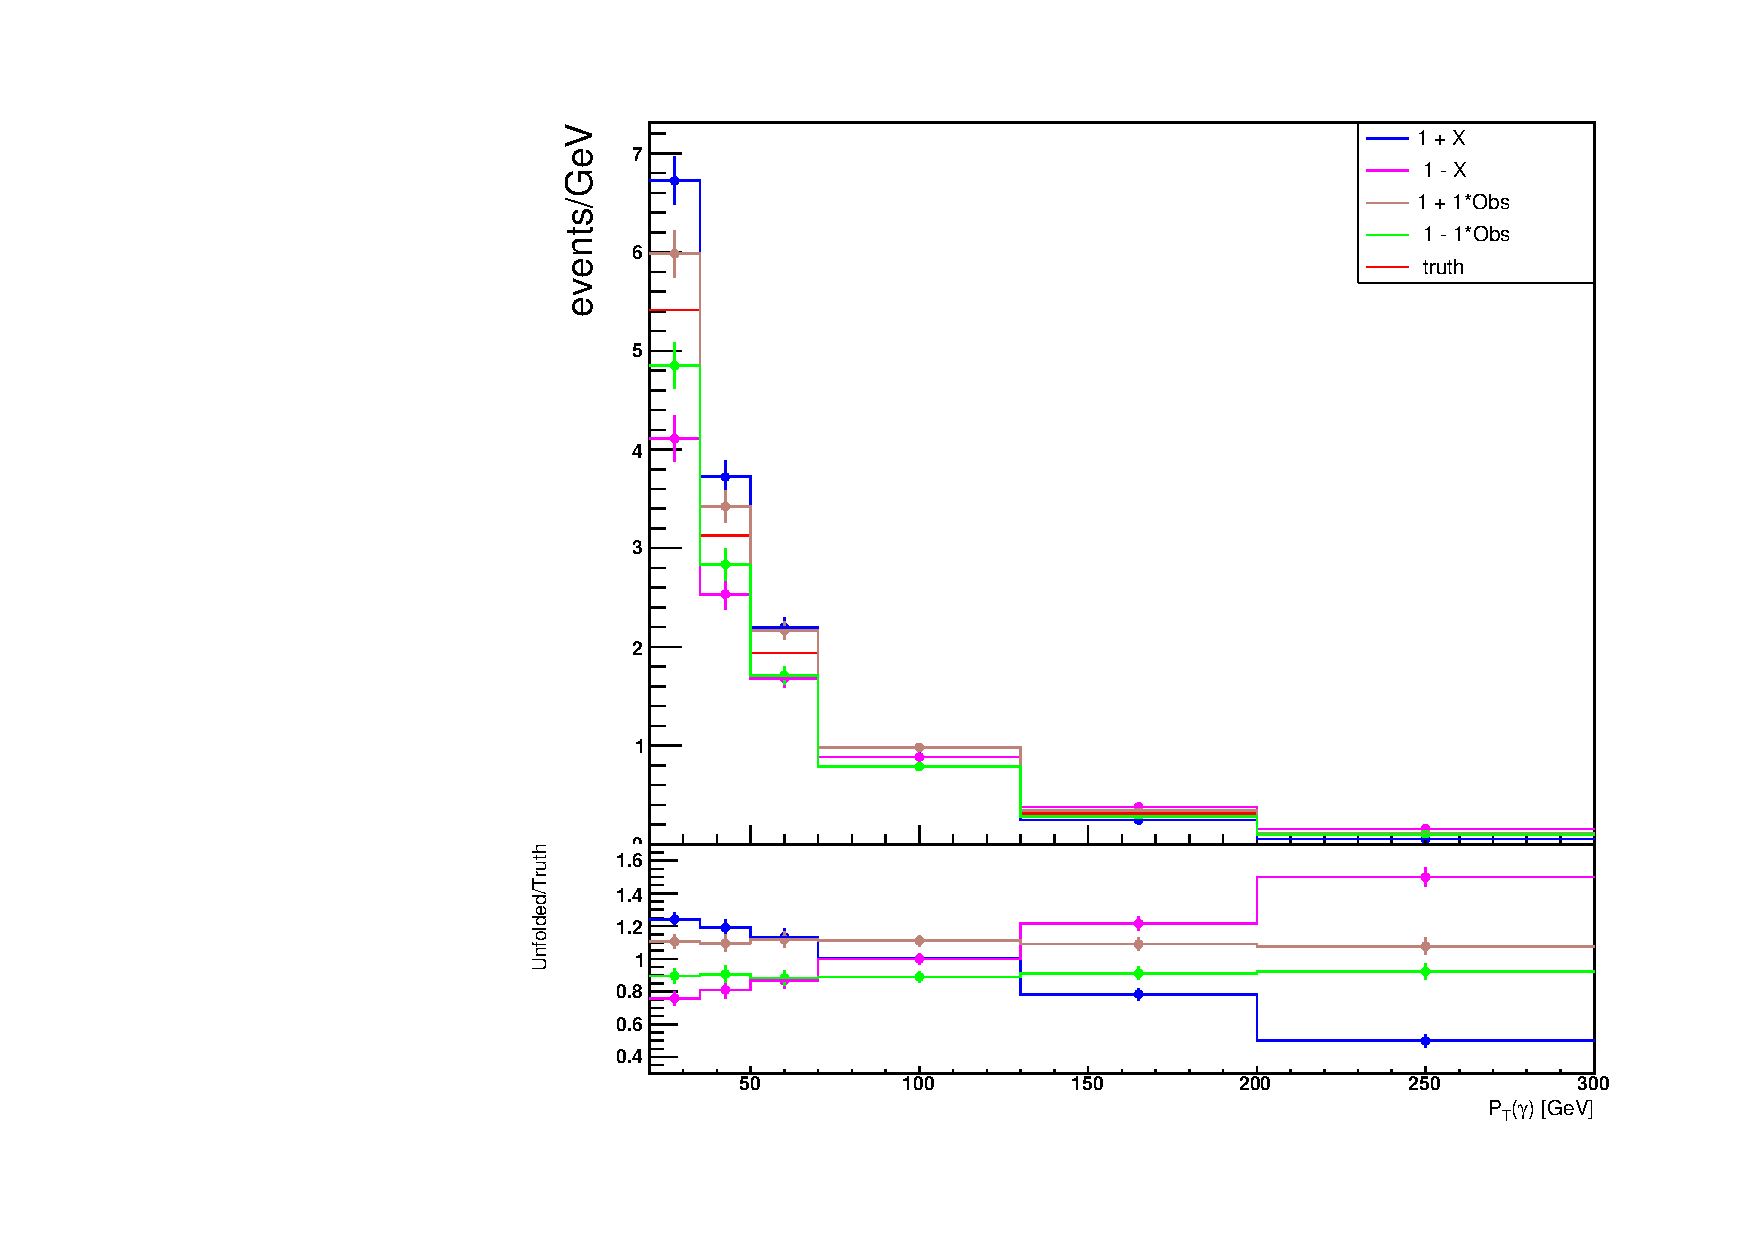
\includegraphics[width=0.4\textwidth]{figures/diff_xsec/ljet/Unfolding_tests/Stress_test/tty1l_pt_all_stat.pdf}}
  \quad\quad
  \subfloat[]{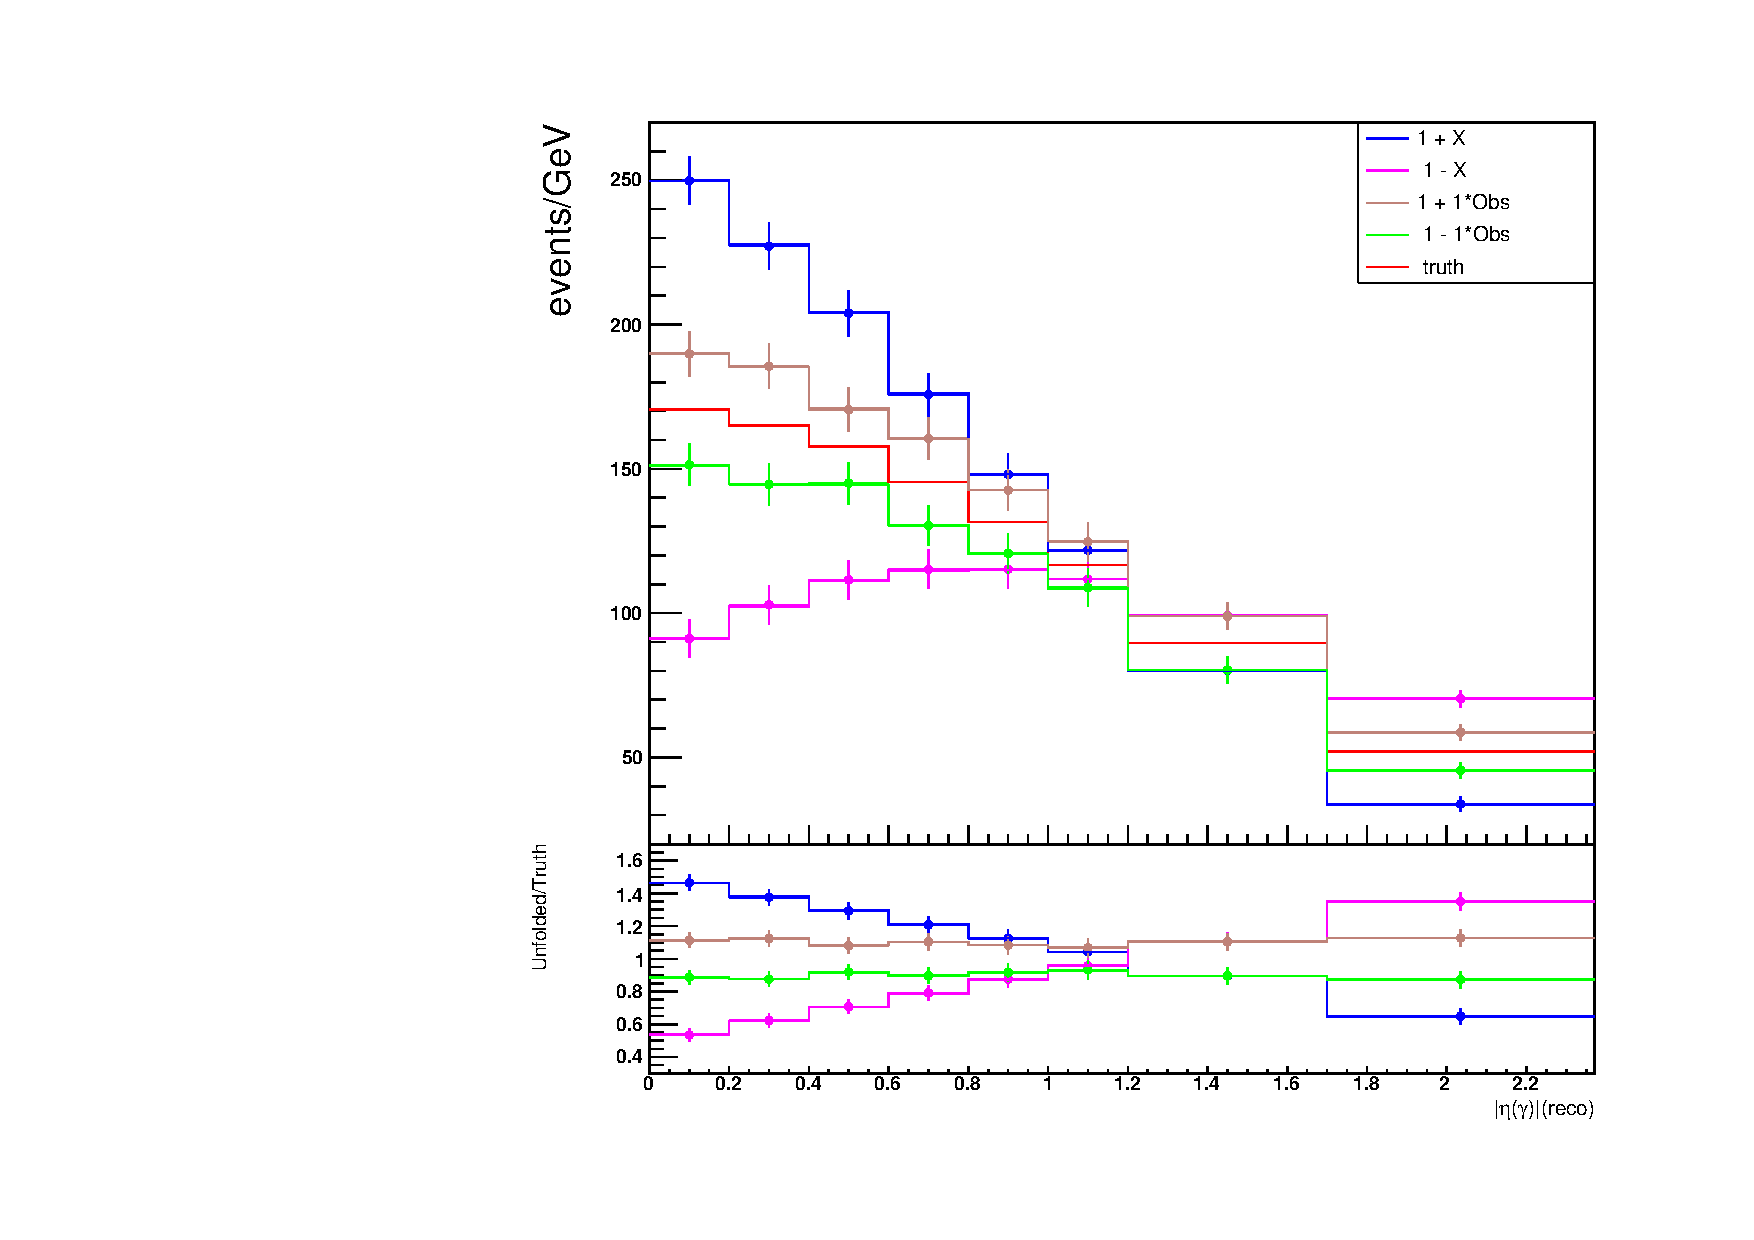
\includegraphics[width=0.4\textwidth]{figures/diff_xsec/ljet/Unfolding_tests/Stress_test/tty1l_eta_all_stat.pdf}}
  \quad\quad
  \subfloat[]{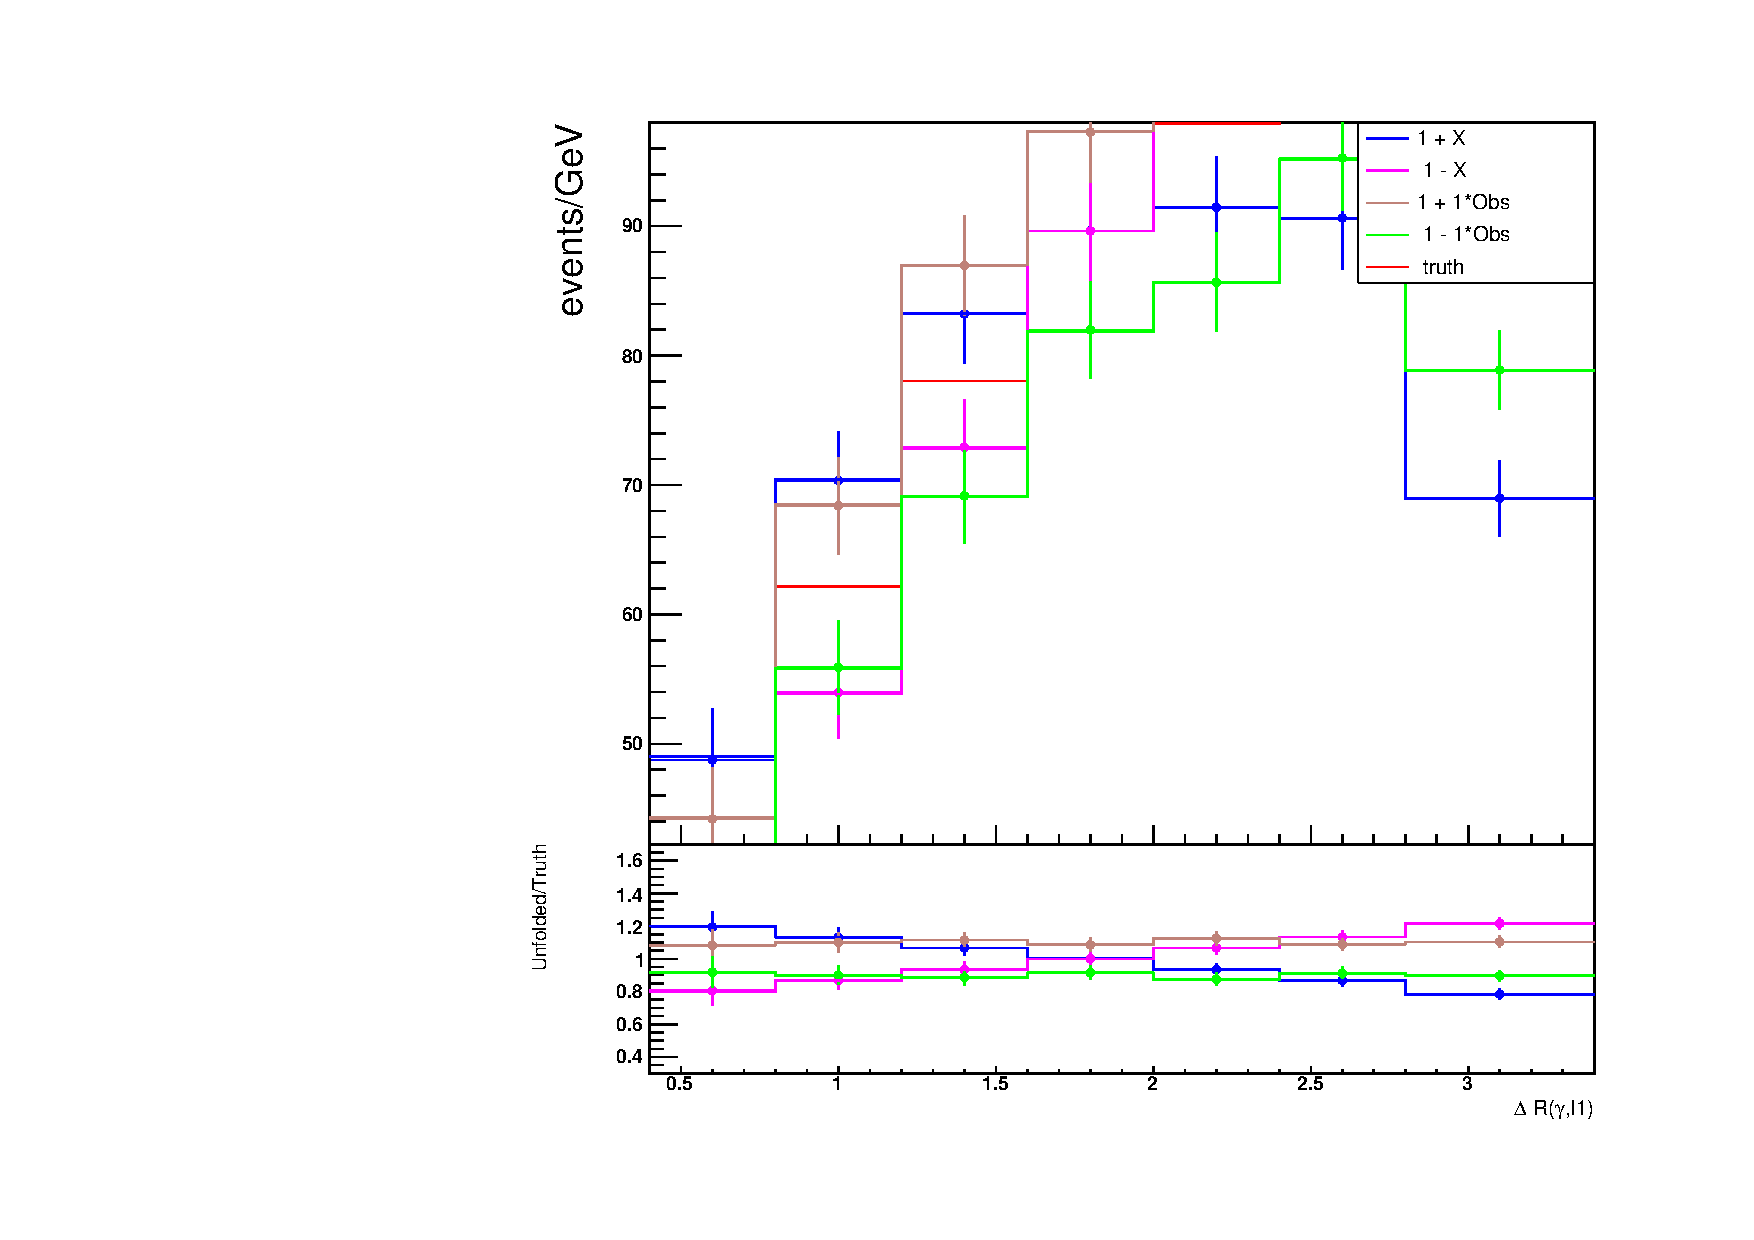
\includegraphics[width=0.4\textwidth]{figures/diff_xsec/ljet/Unfolding_tests/Stress_test/tty1l_dr_all_stat.pdf}}
  \quad\quad
  \subfloat[]{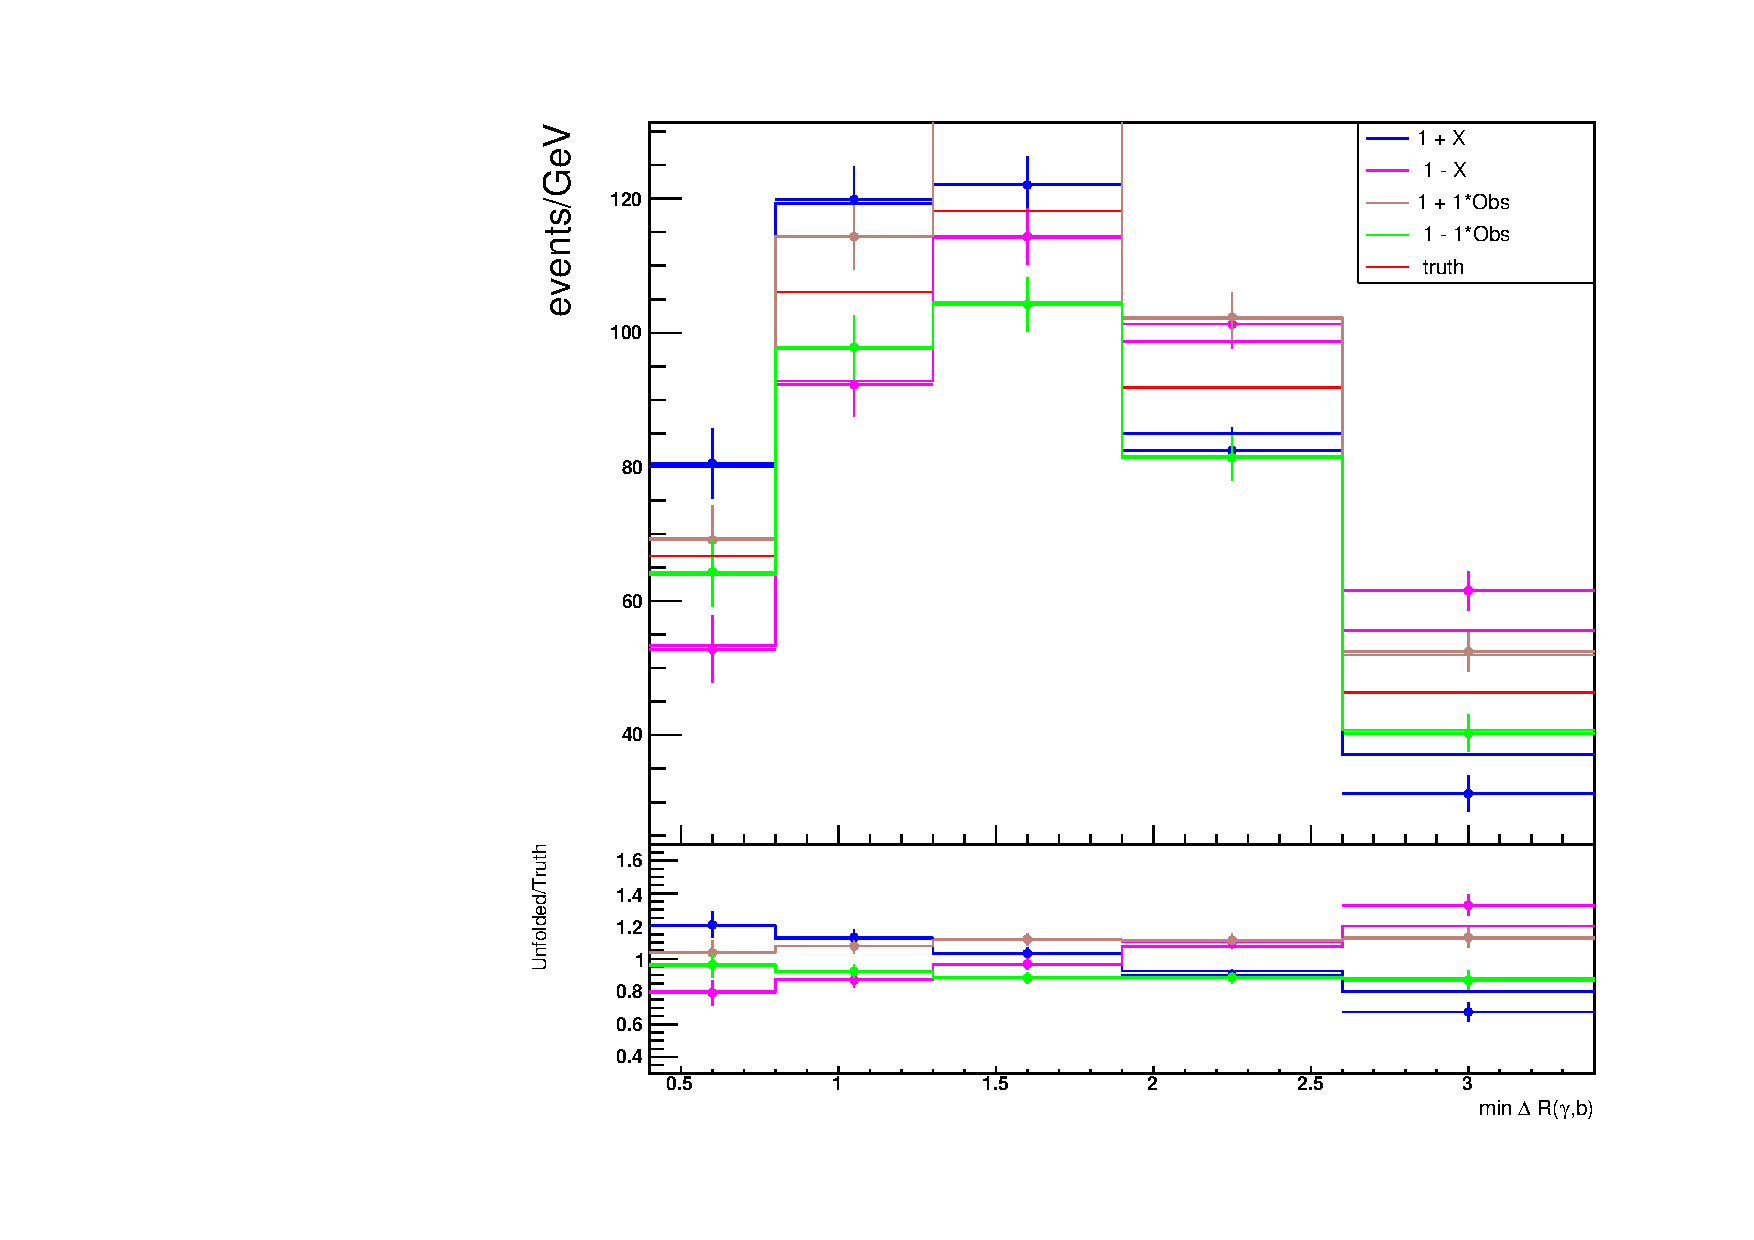
\includegraphics[width=0.4\textwidth]{figures/diff_xsec/ljet/Unfolding_tests/Stress_test/tty1l_drphb_all_stat.pdf}}
  \quad\quad
  \subfloat[]{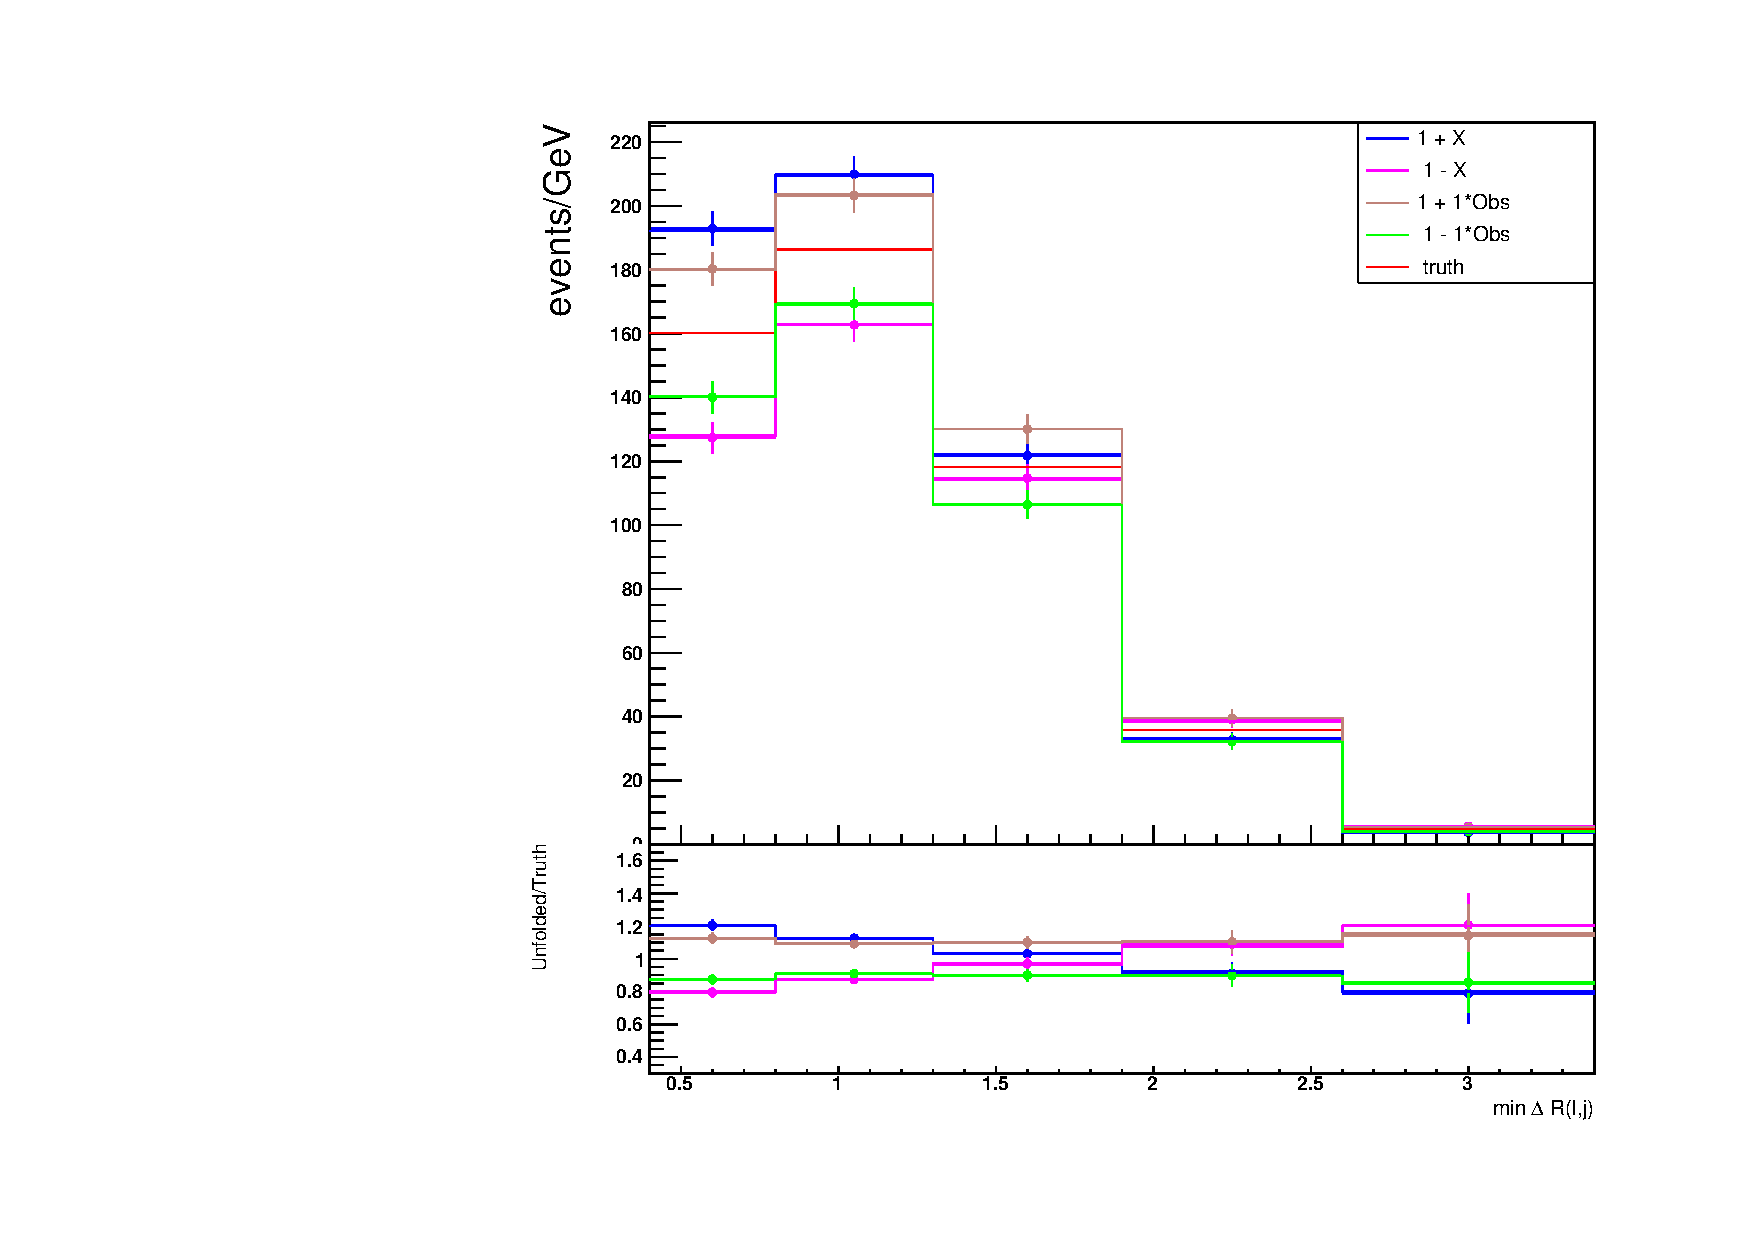
\includegraphics[width=0.4\textwidth]{figures/diff_xsec/ljet/Unfolding_tests/Stress_test/tty1l_drlj_all_stat.pdf}}
  \subfloat[]{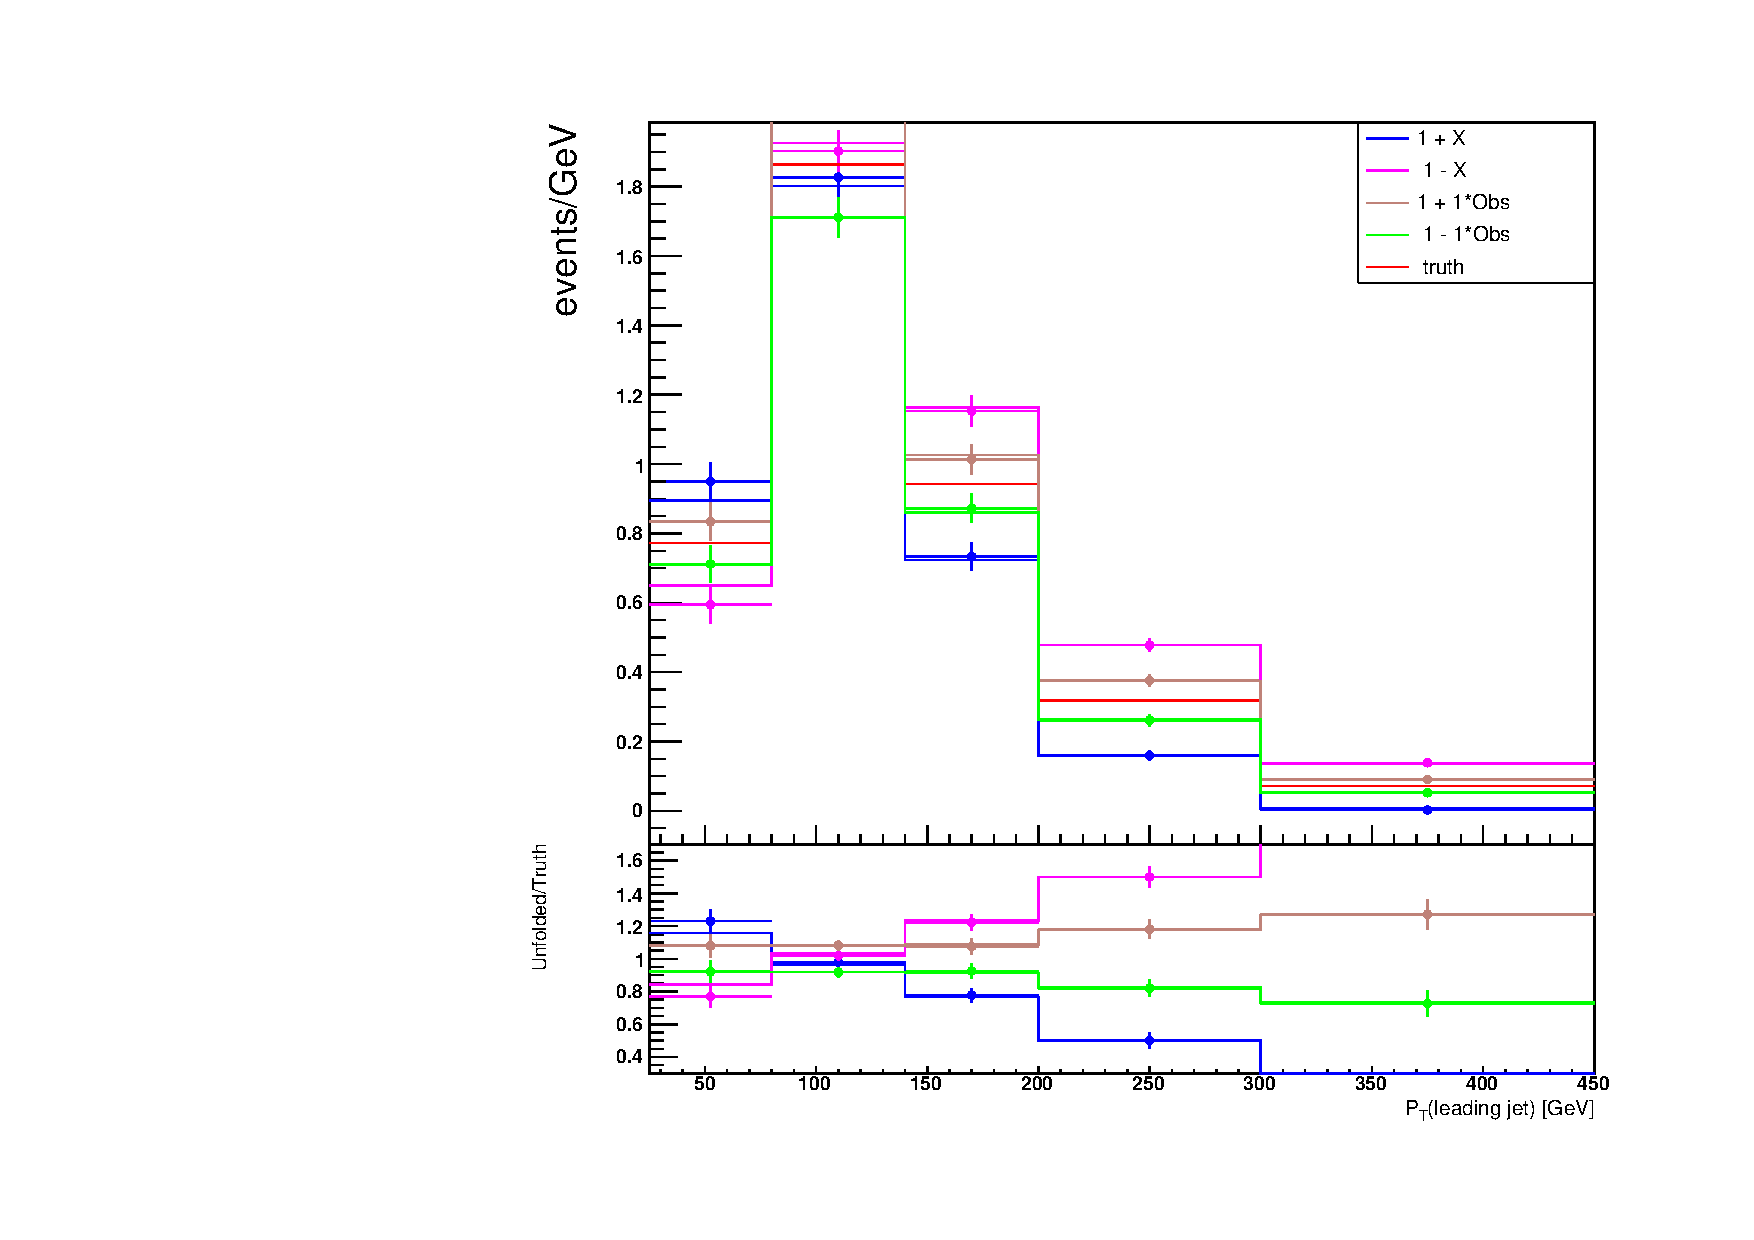
\includegraphics[width=0.4\textwidth]{figures/diff_xsec/ljet/Unfolding_tests/Stress_test/tty1l_ptj1_all_stat.pdf}}
  \caption{Stress test for the five observables in the single lepton channel for \tty production measurement. Both the dots and lines are ratios made with respect to the nominal particle level.The dots are the ratio of the unfolded reweighted distributions to the nominal particle level distribution, while the solid lines are the ratio of the reweighted particle level distributions to the nominal one. X is defined in previous section. The uncertainty bars displayed in the plots represent only he statistical error considered in the unfolding.}
  \label{fig:unfolded_ljet_dist_stress_test}
\end{figure}
\FloatBarrier


\begin{figure}[ht]
  \centering
  \subfloat[]{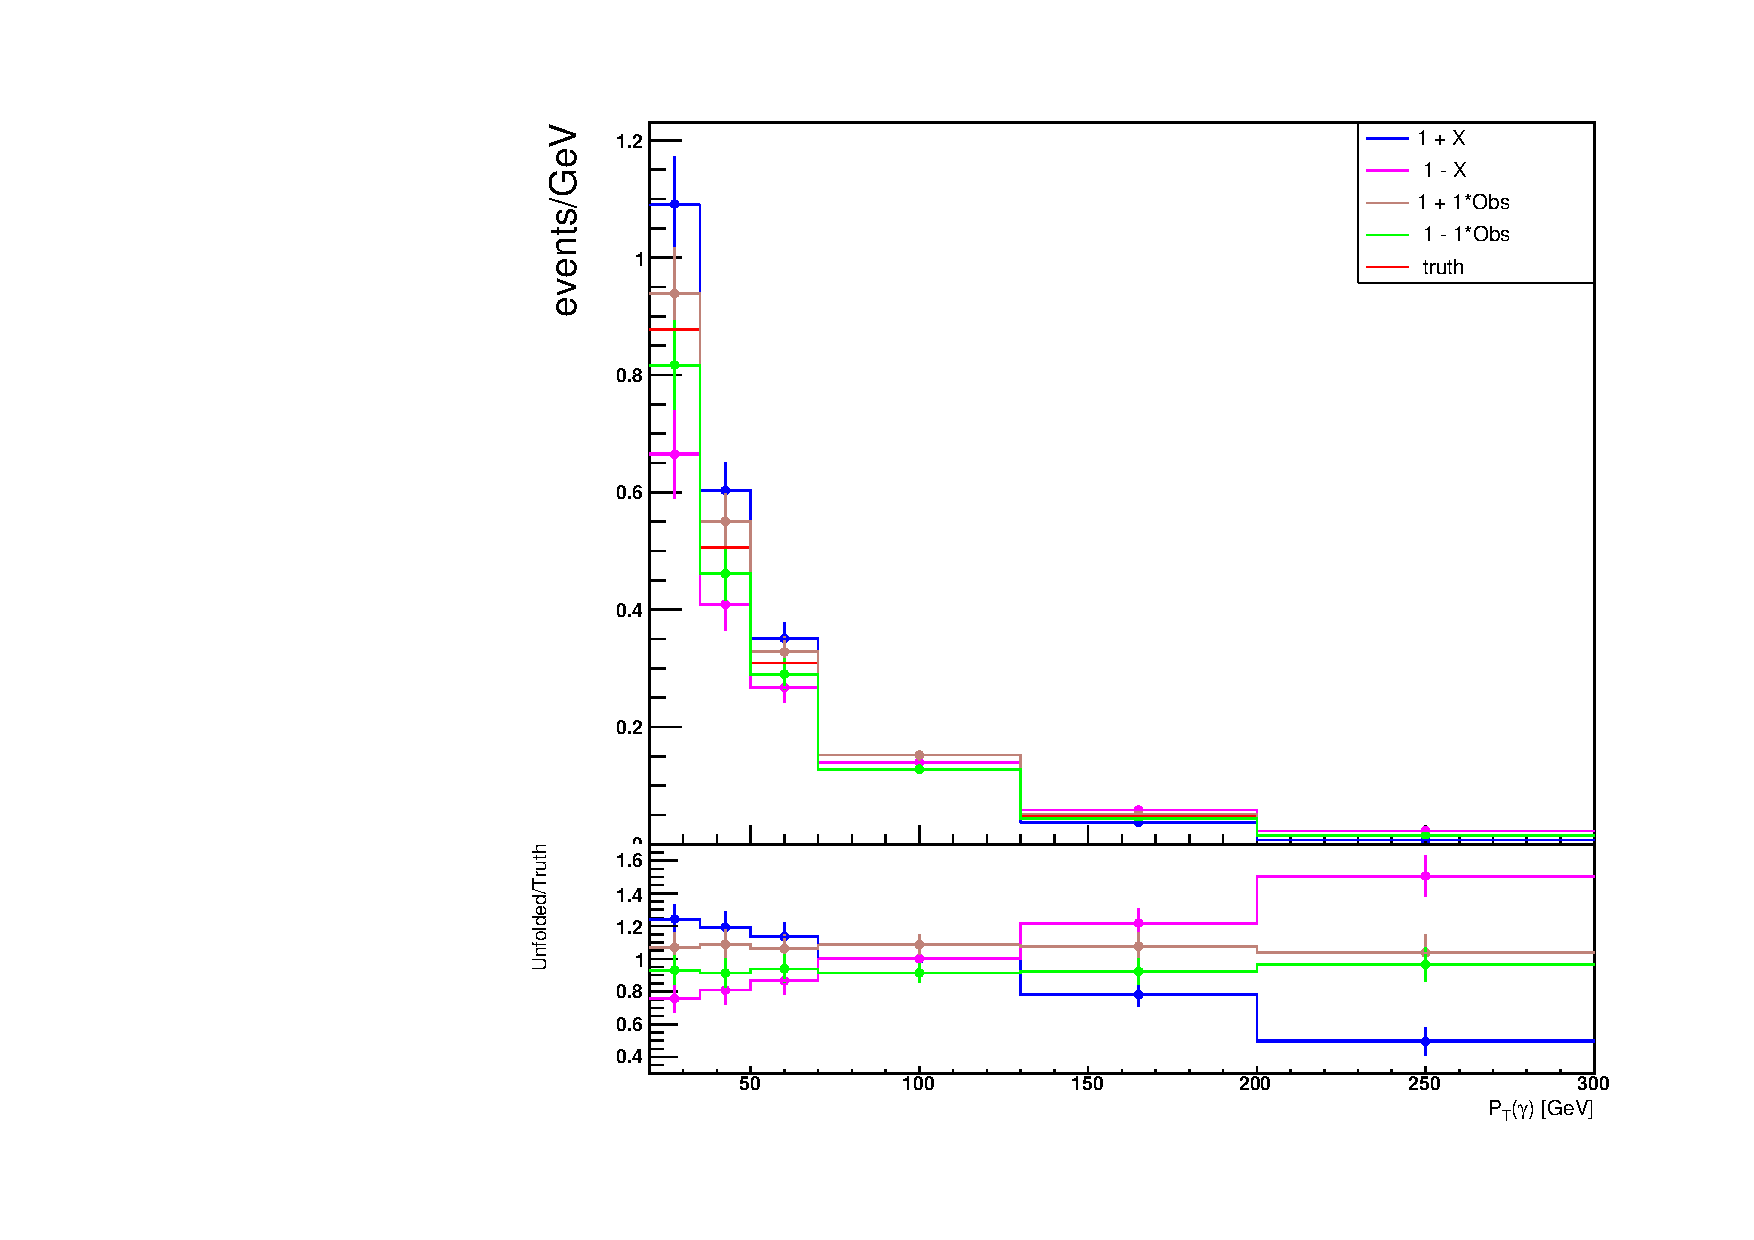
\includegraphics[width=0.4\textwidth]{figures/diff_xsec/dilep/Unfolding_tests/Stress_test/tty2l_pt_all_stat.pdf}}
  \quad\quad
  \subfloat[]{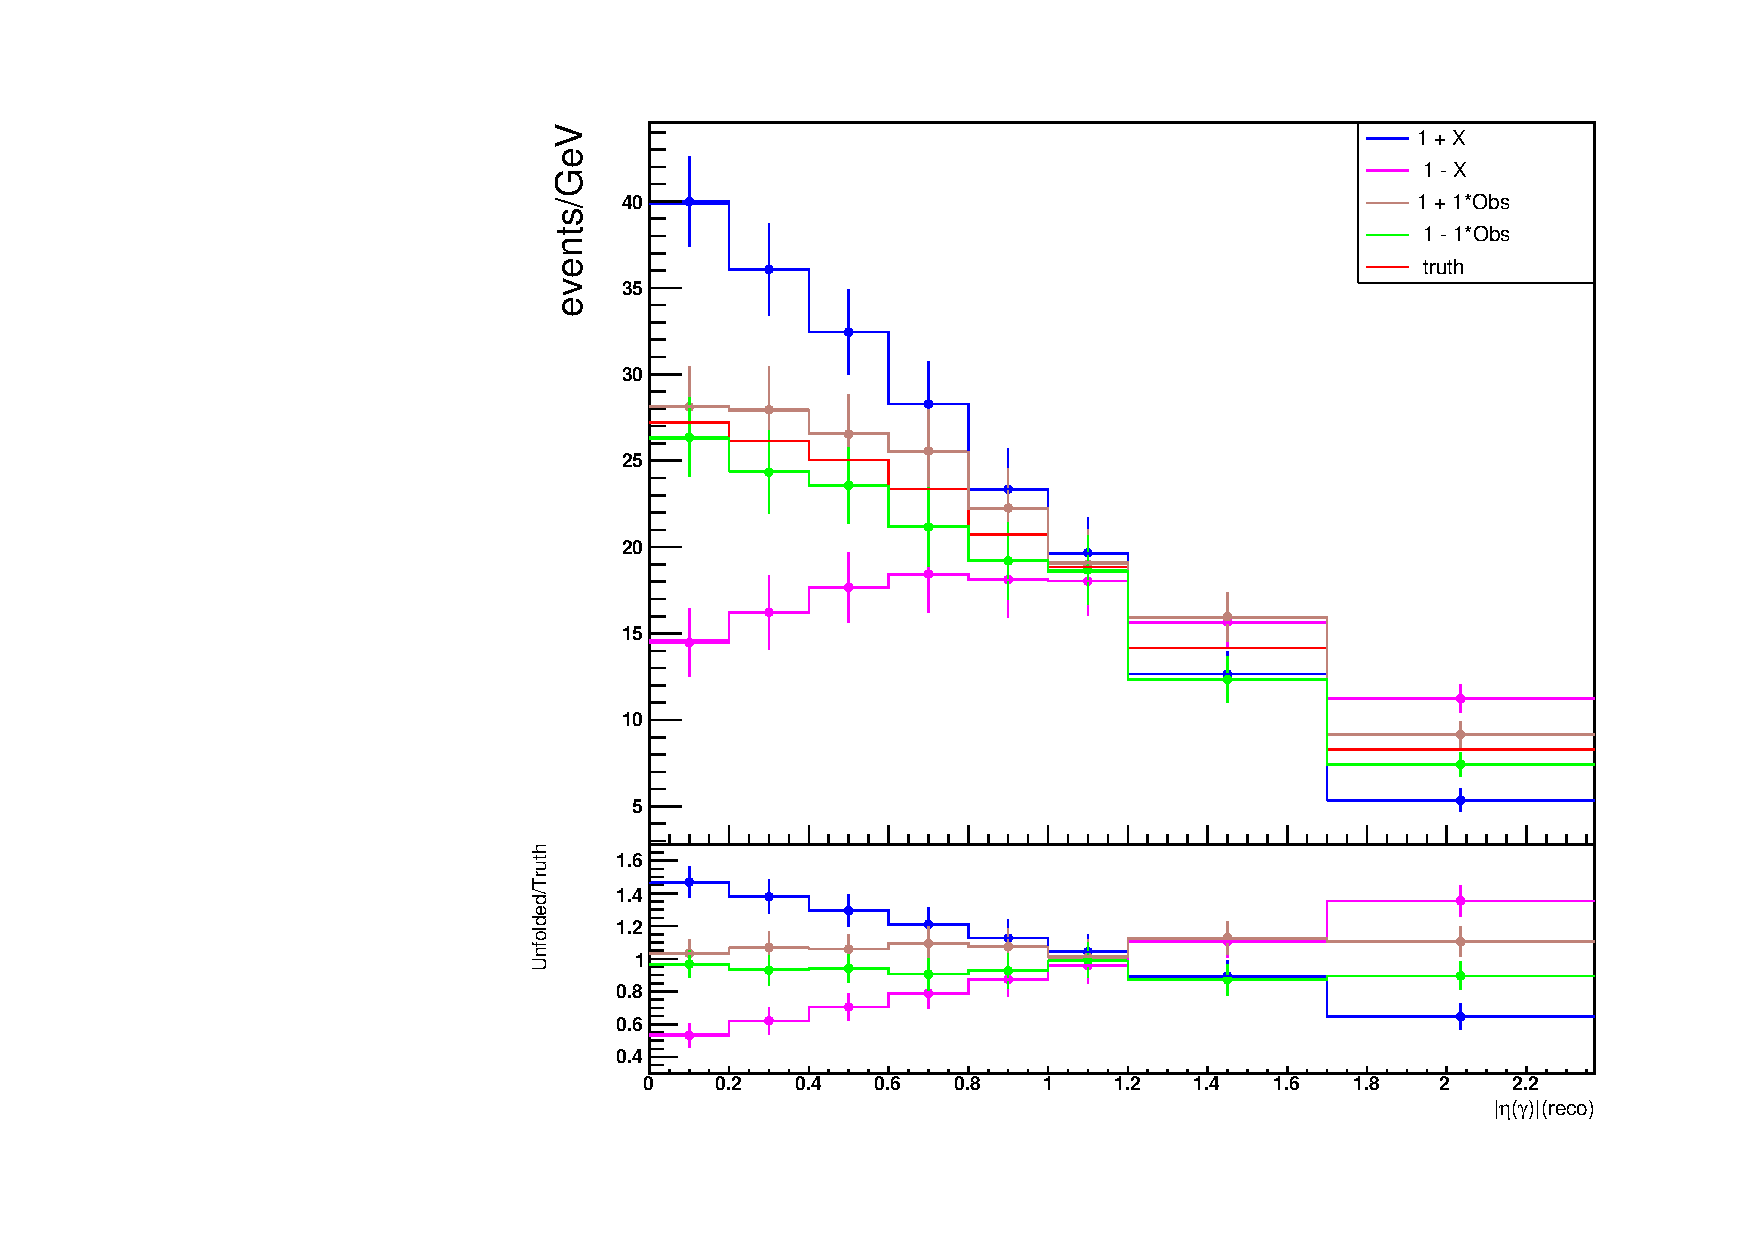
\includegraphics[width=0.4\textwidth]{figures/diff_xsec/dilep/Unfolding_tests/Stress_test/tty2l_eta_all_stat.pdf}}
  \quad\quad
  \subfloat[]{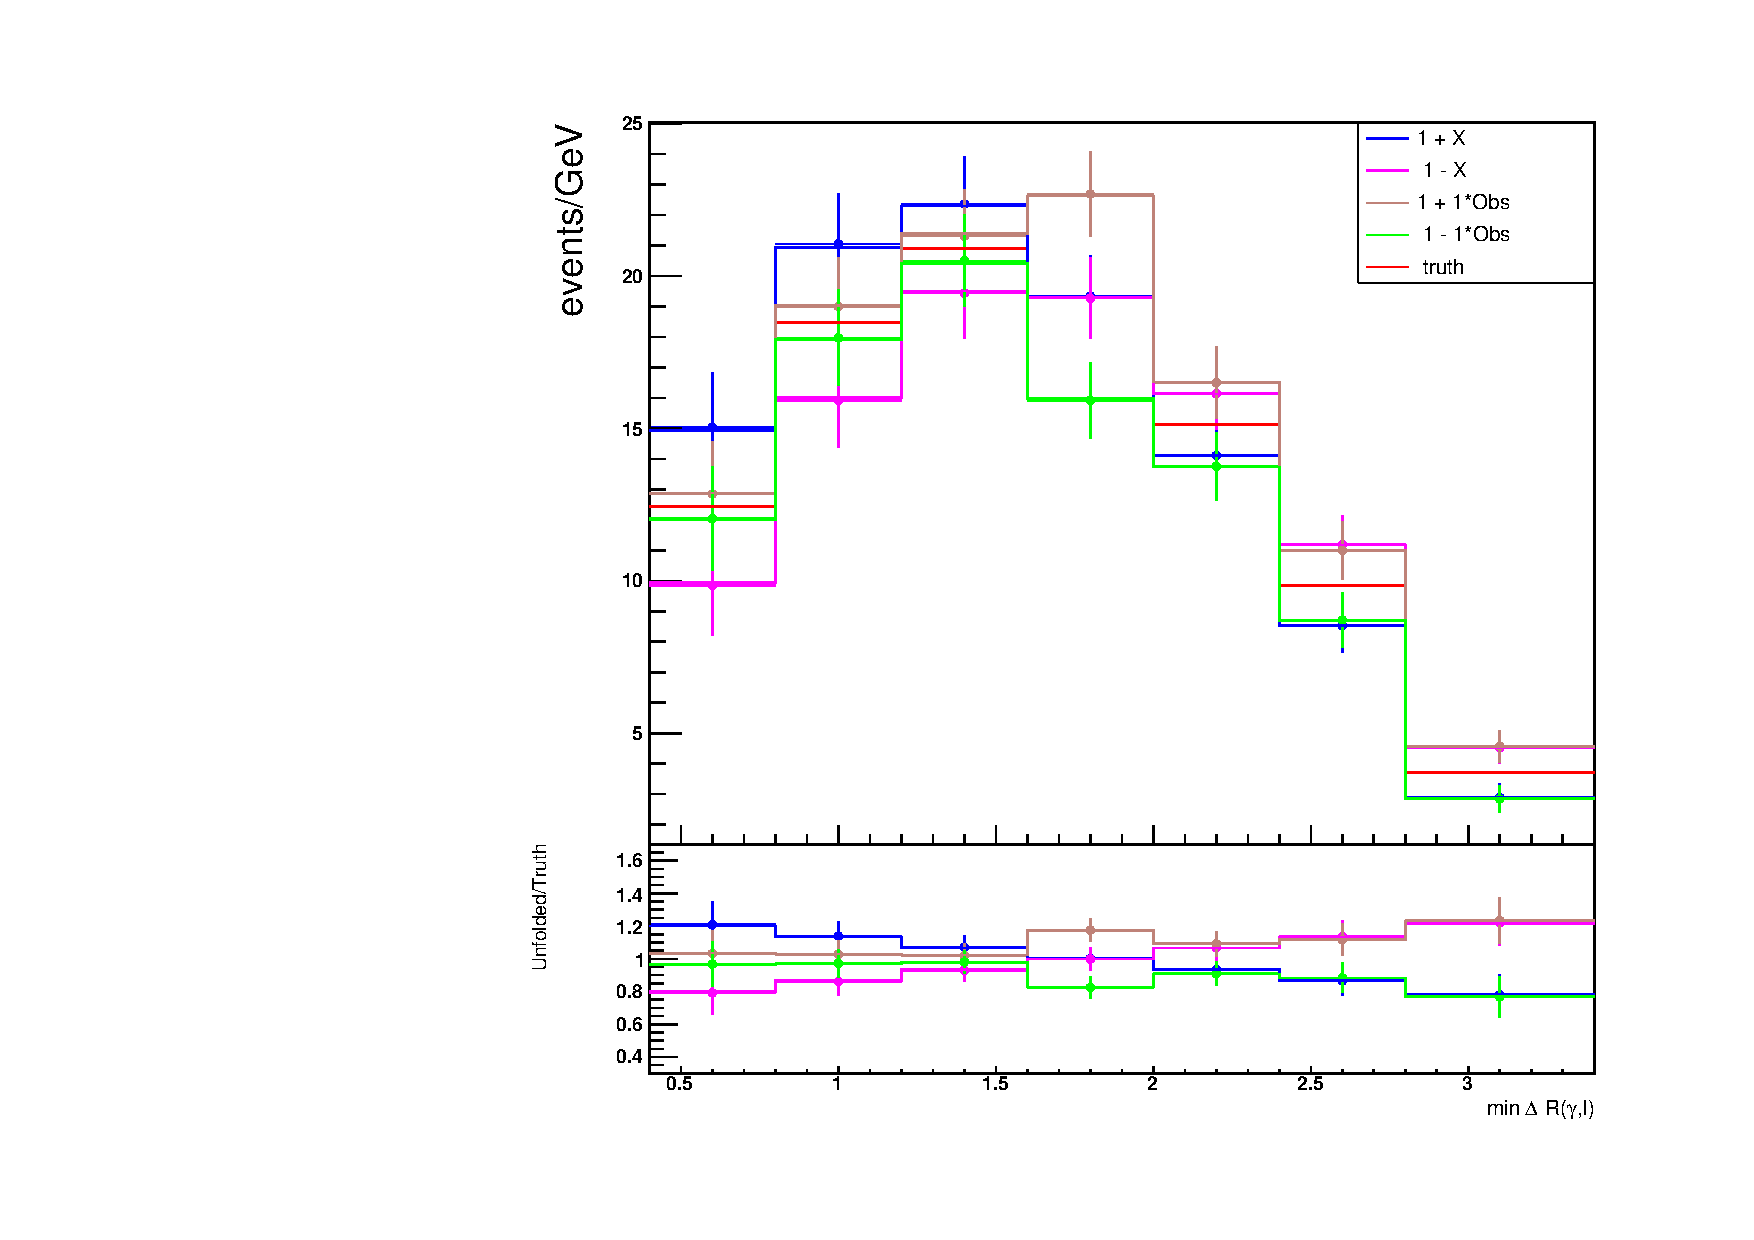
\includegraphics[width=0.4\textwidth]{figures/diff_xsec/dilep/Unfolding_tests/Stress_test/tty2l_dr_all_stat.pdf}}
  \quad\quad
  \subfloat[]{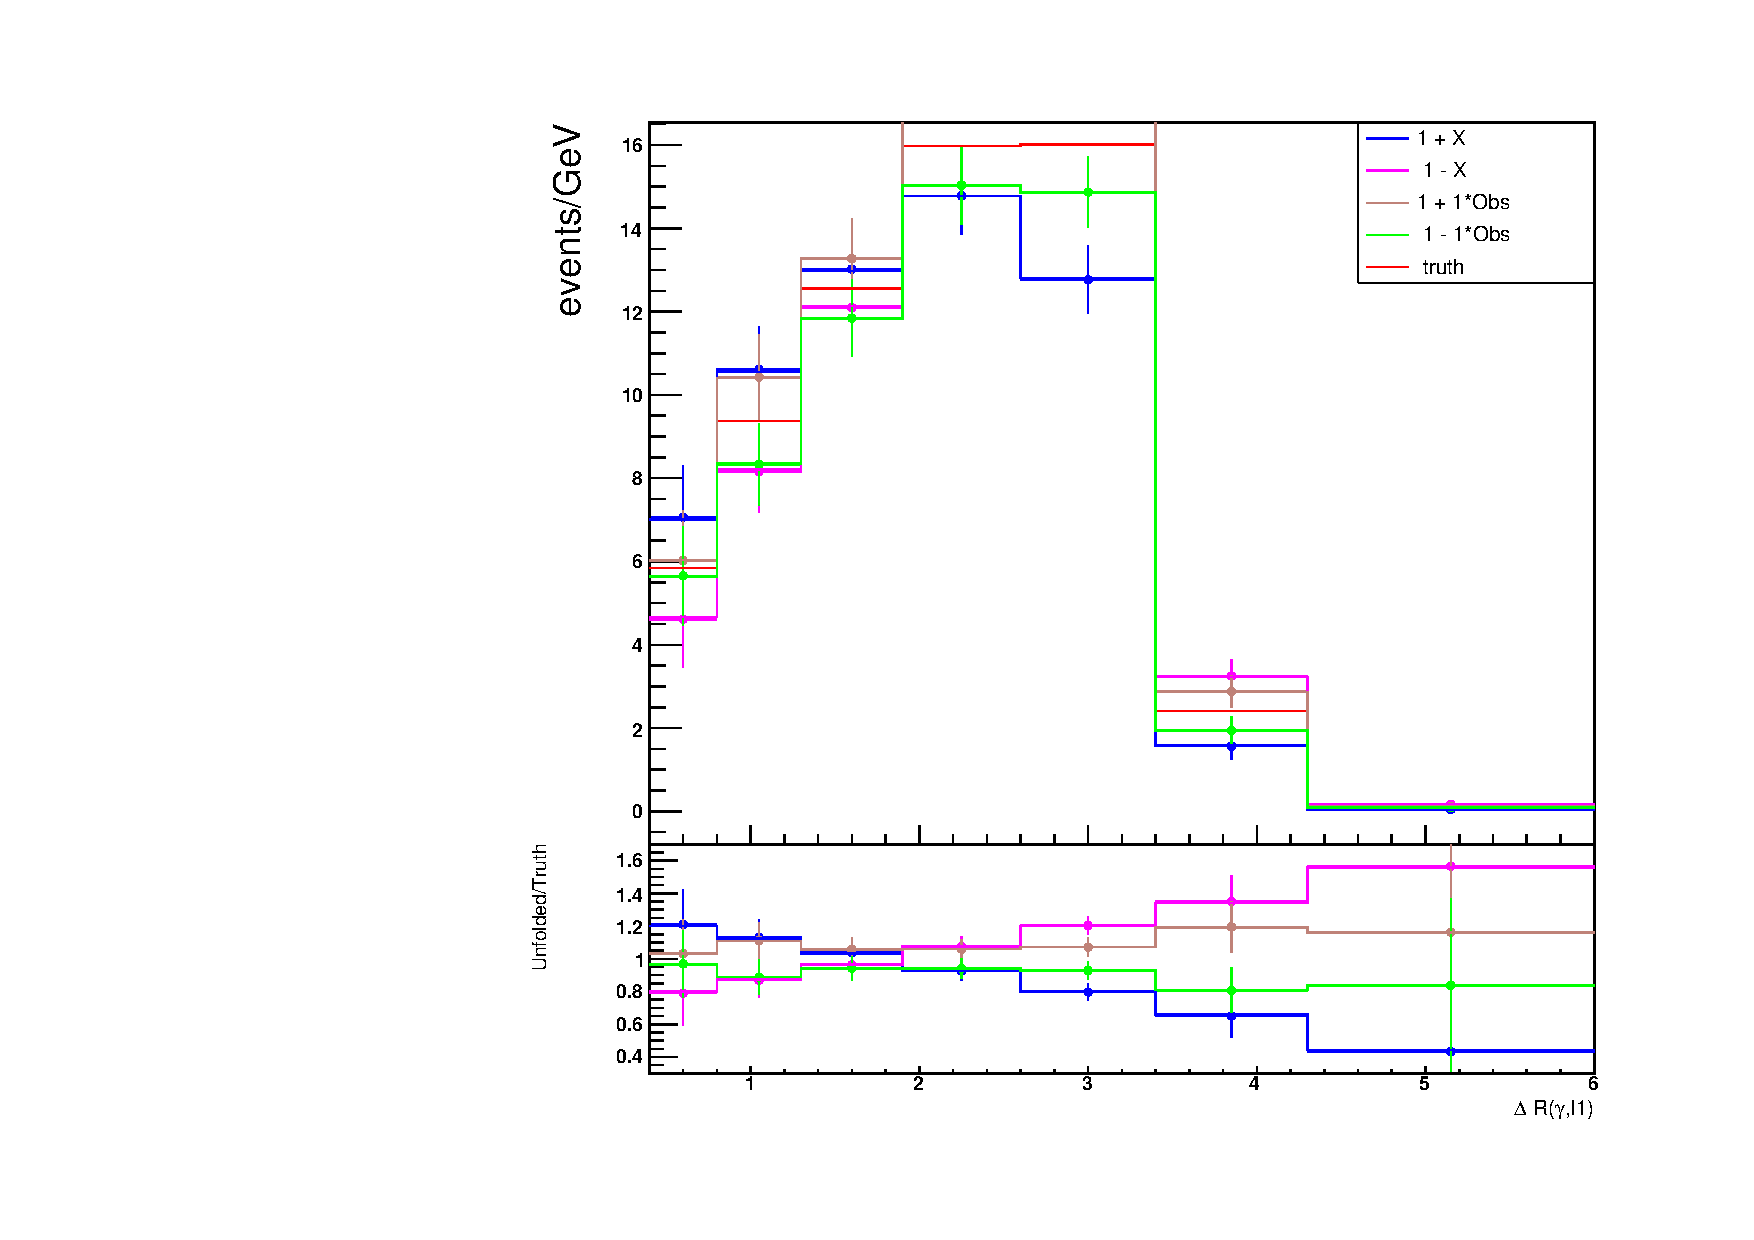
\includegraphics[width=0.4\textwidth]{figures/diff_xsec/dilep/Unfolding_tests/Stress_test/tty2l_dr1_all_stat.pdf}}
  \quad\quad
  \subfloat[]{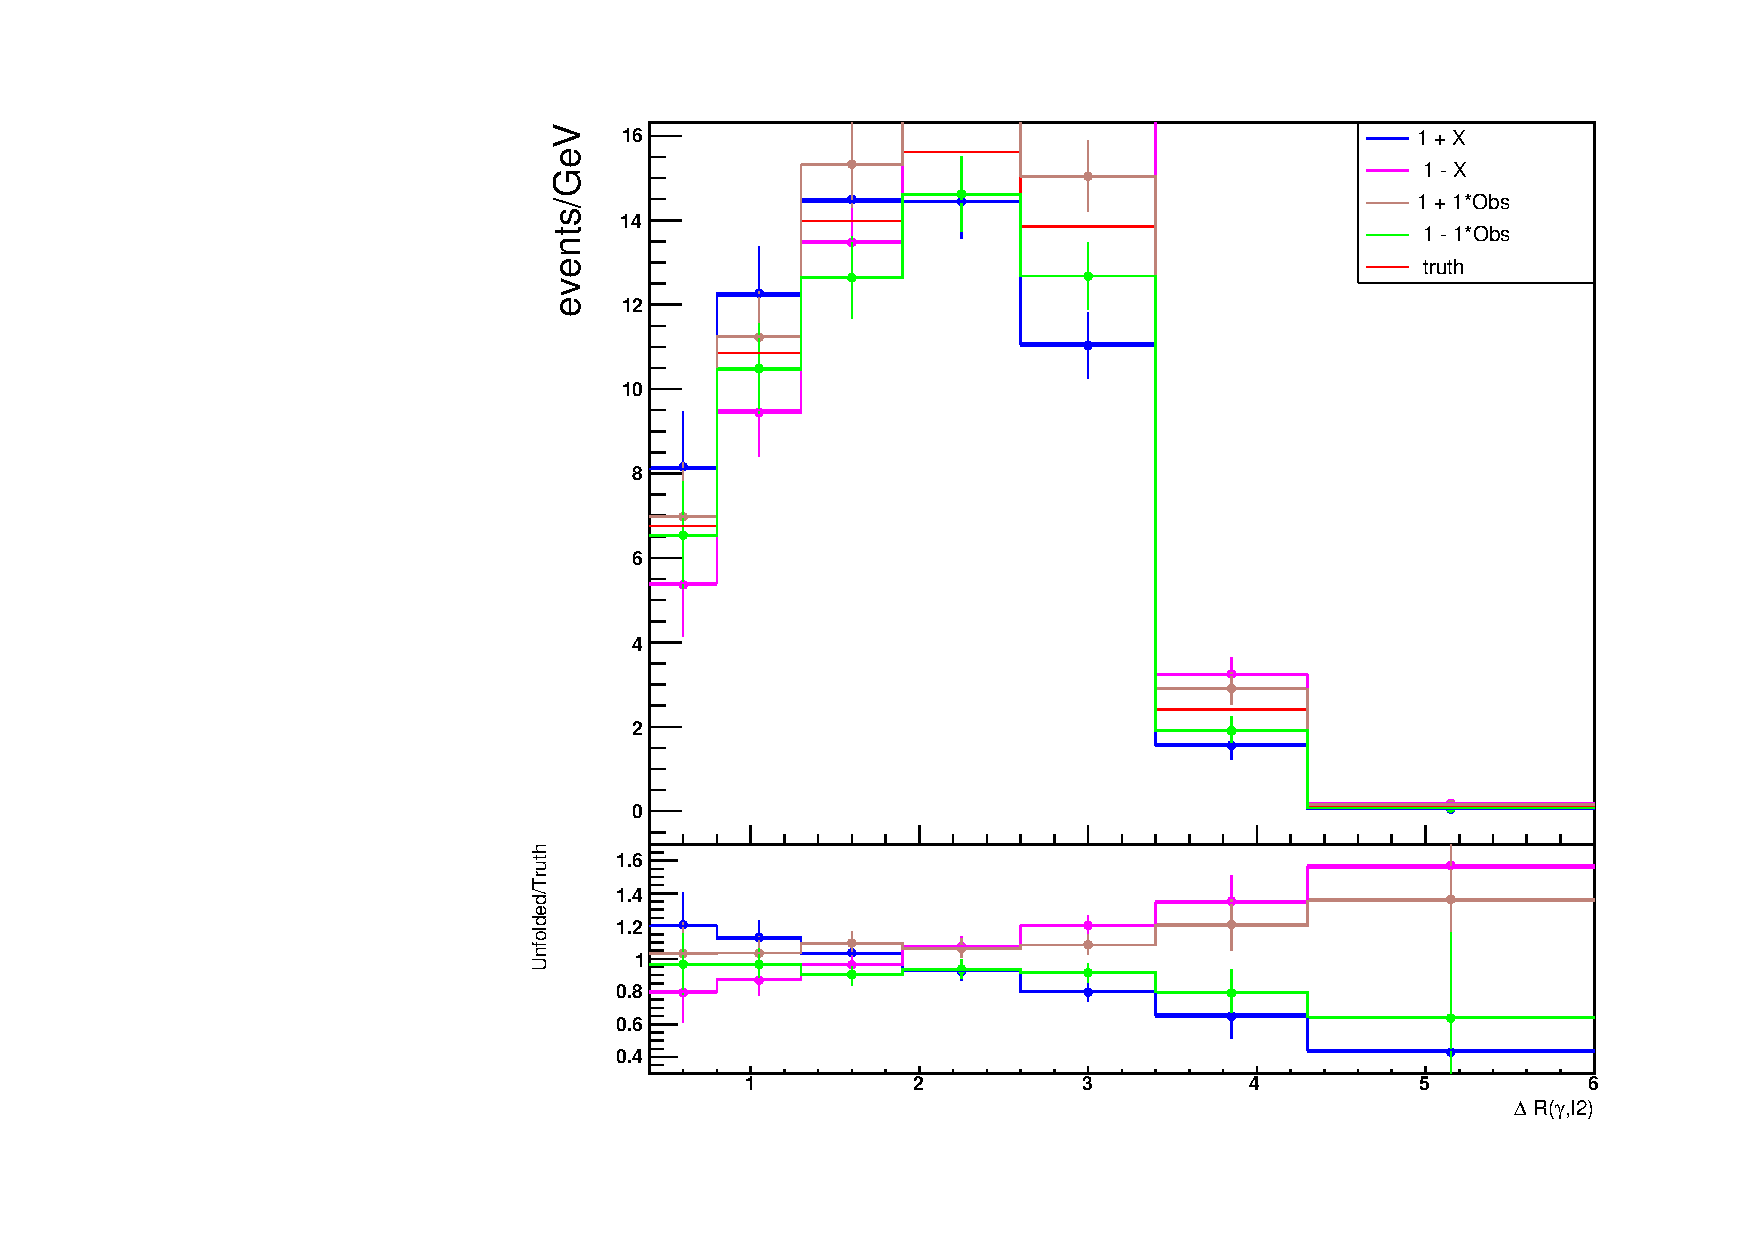
\includegraphics[width=0.4\textwidth]{figures/diff_xsec/dilep/Unfolding_tests/Stress_test/tty2l_dr2_all_stat.pdf}}
  \quad\quad
  \subfloat[]{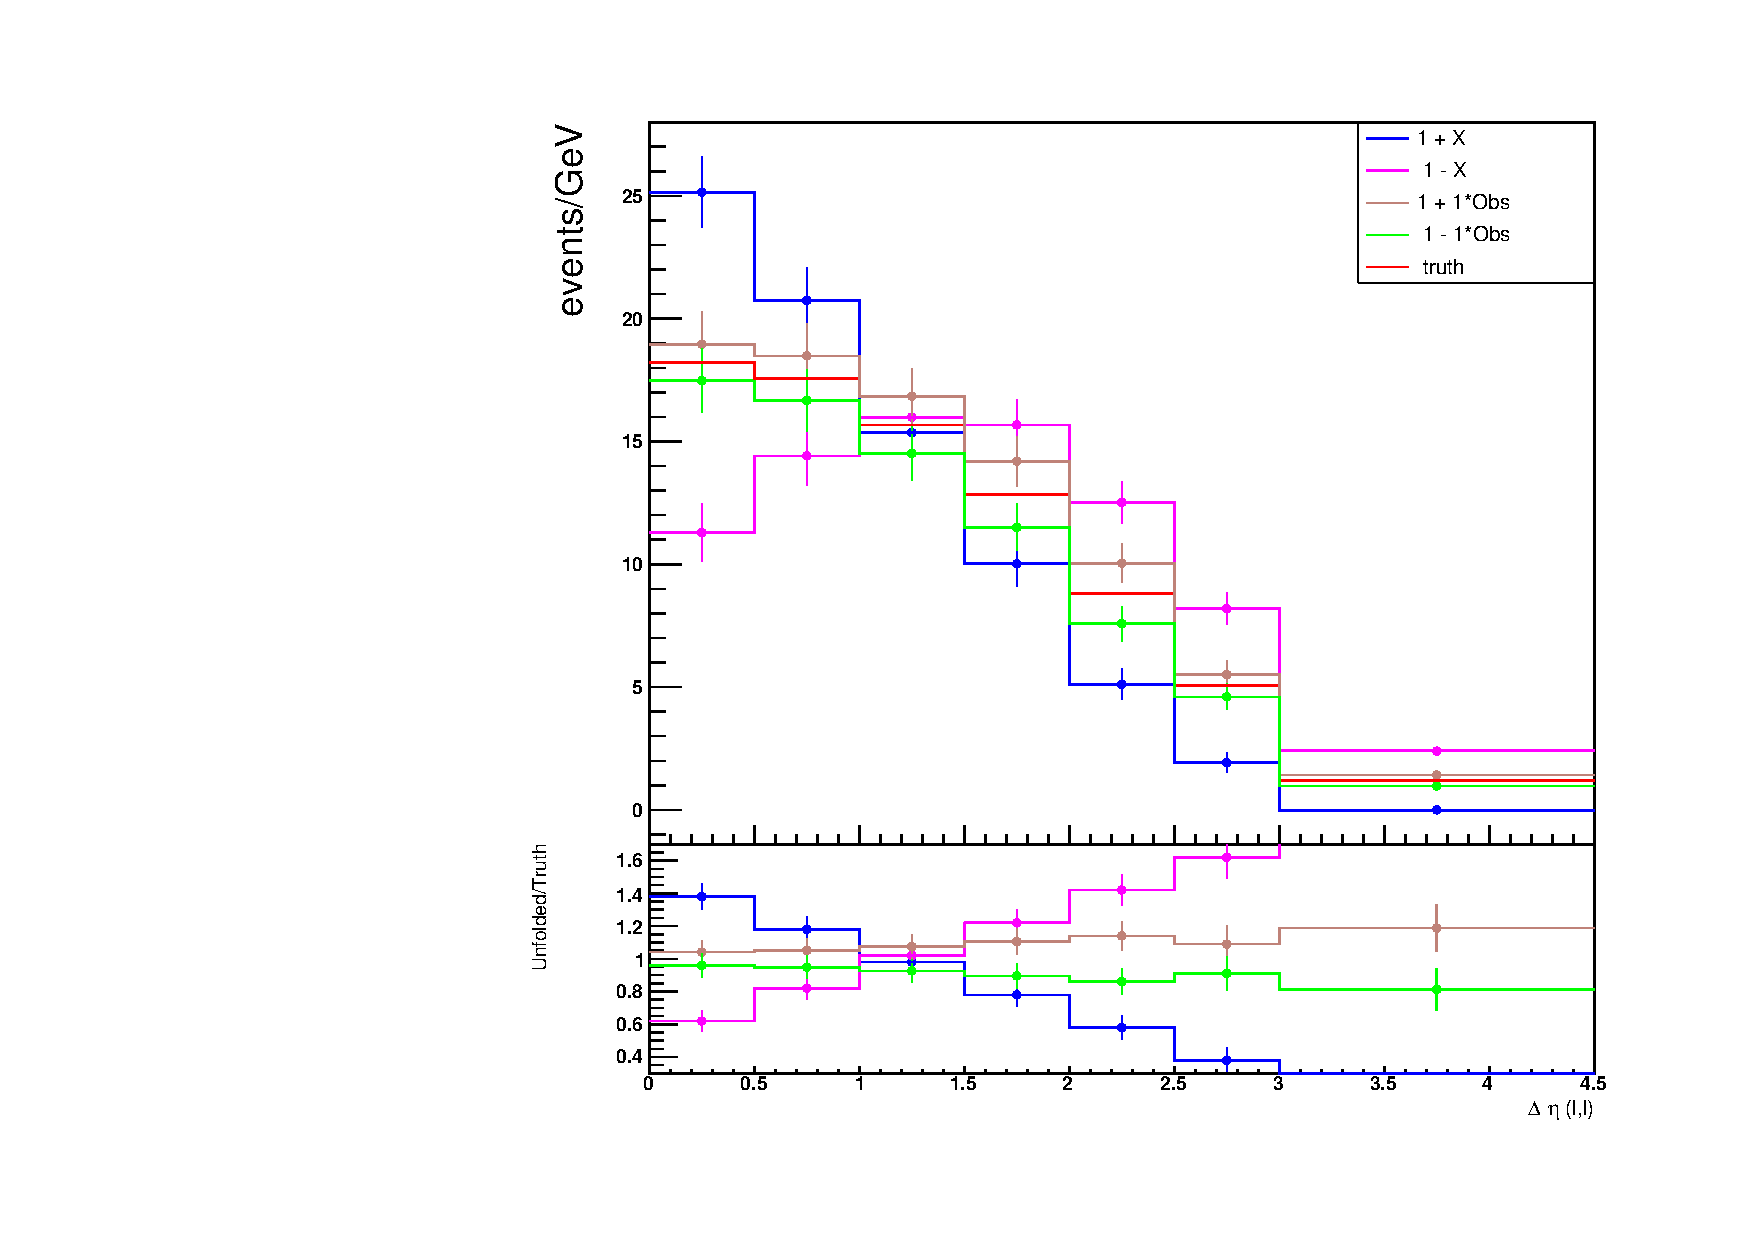
\includegraphics[width=0.4\textwidth]{figures/diff_xsec/dilep/Unfolding_tests/Stress_test/tty2l_dEtall_all_stat.pdf}}
  \caption{Stress test for the five observables in the dilepton channel for \tty production measurement. Both the dots and lines are ratios made with respect to the nominal particle level.The dots are the ratio of the unfolded reweighted distributions to the nominal particle level distribution, while the solid lines are the ratio of the reweighted particle level distributions to the nominal one. X is defined in previous section. The uncertainty bars displayed in the plots represent only the statistical error considered in the unfolding.}
  \label{fig:unfolded_dilep_dist_stress_test_1}
\end{figure}

\begin{figure}[ht]
  \centering
  \subfloat[]{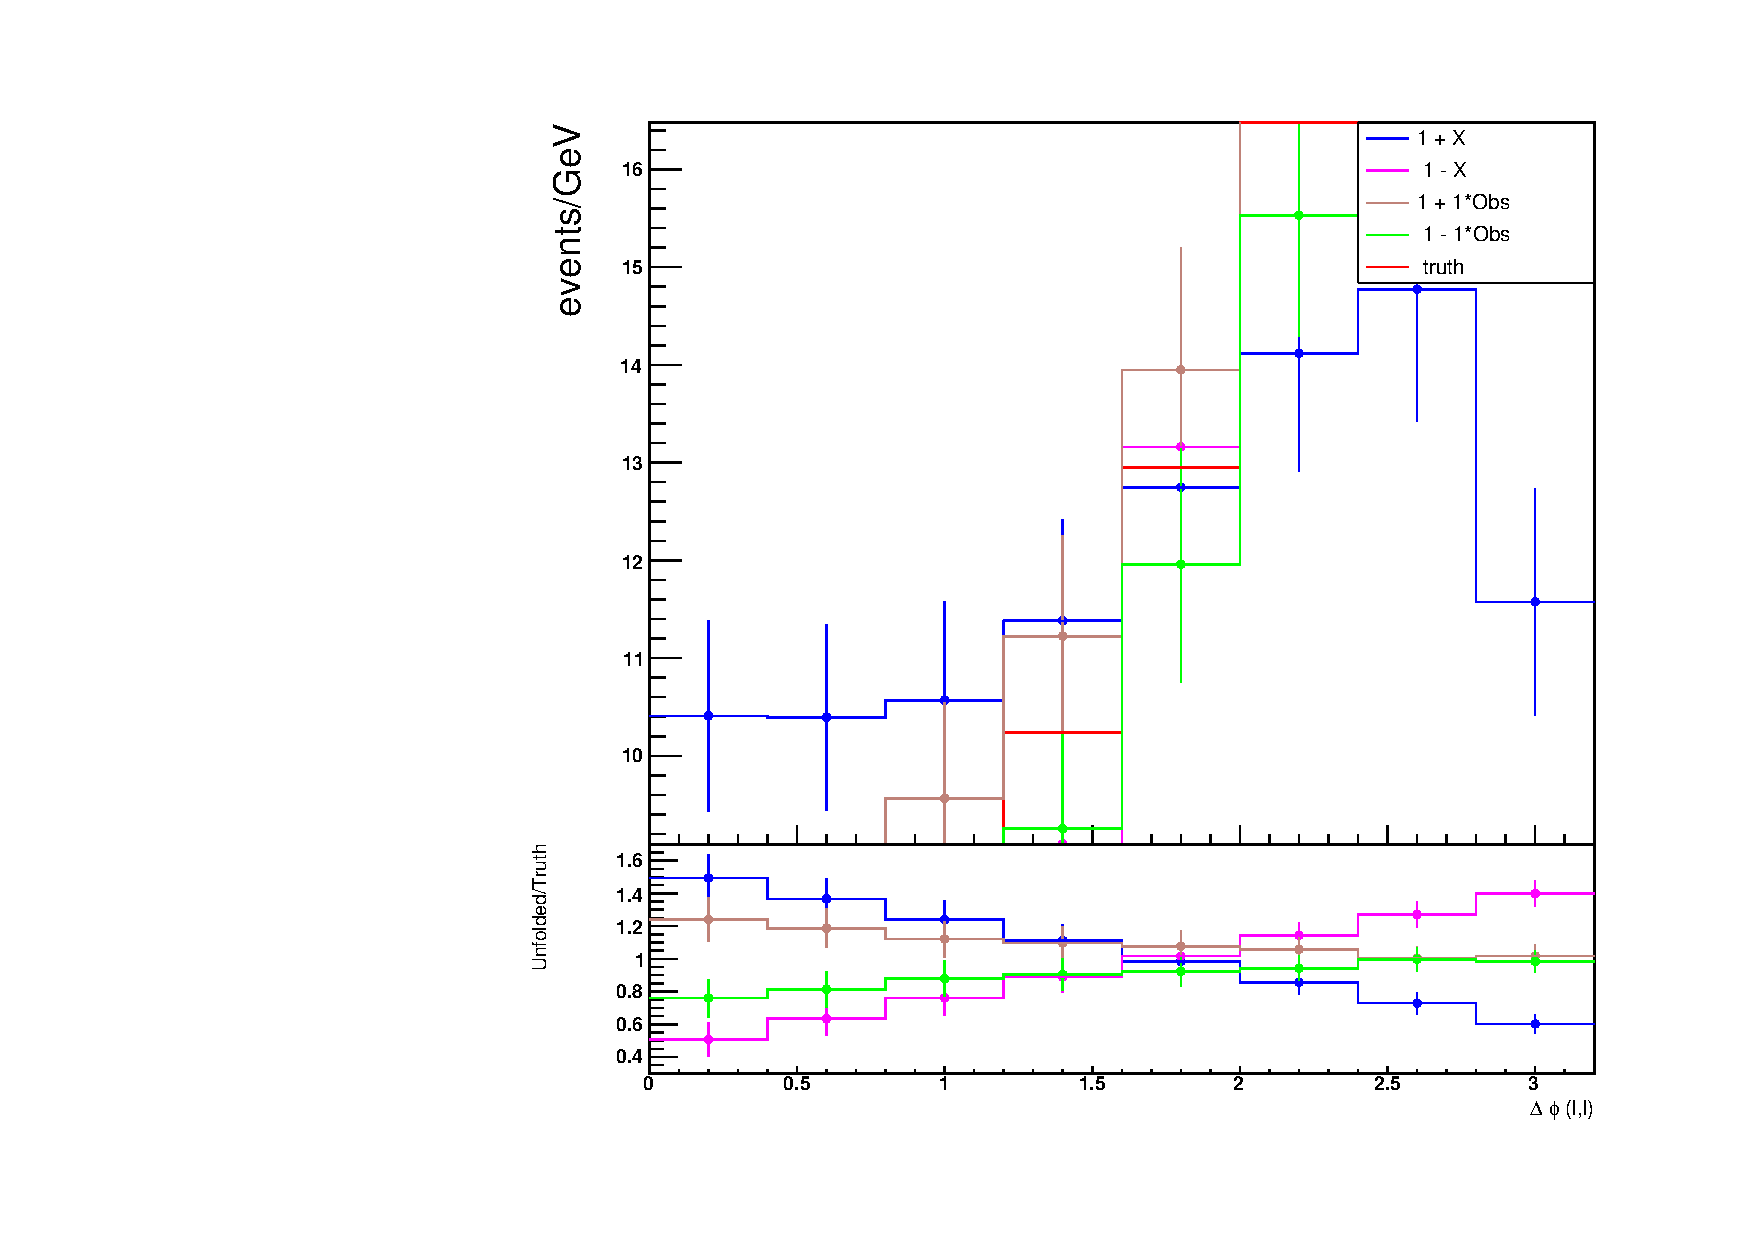
\includegraphics[width=0.4\textwidth]{figures/diff_xsec/dilep/Unfolding_tests/Stress_test/tty2l_dPhill_all_stat.pdf}}
  \quad\quad
  \subfloat[]{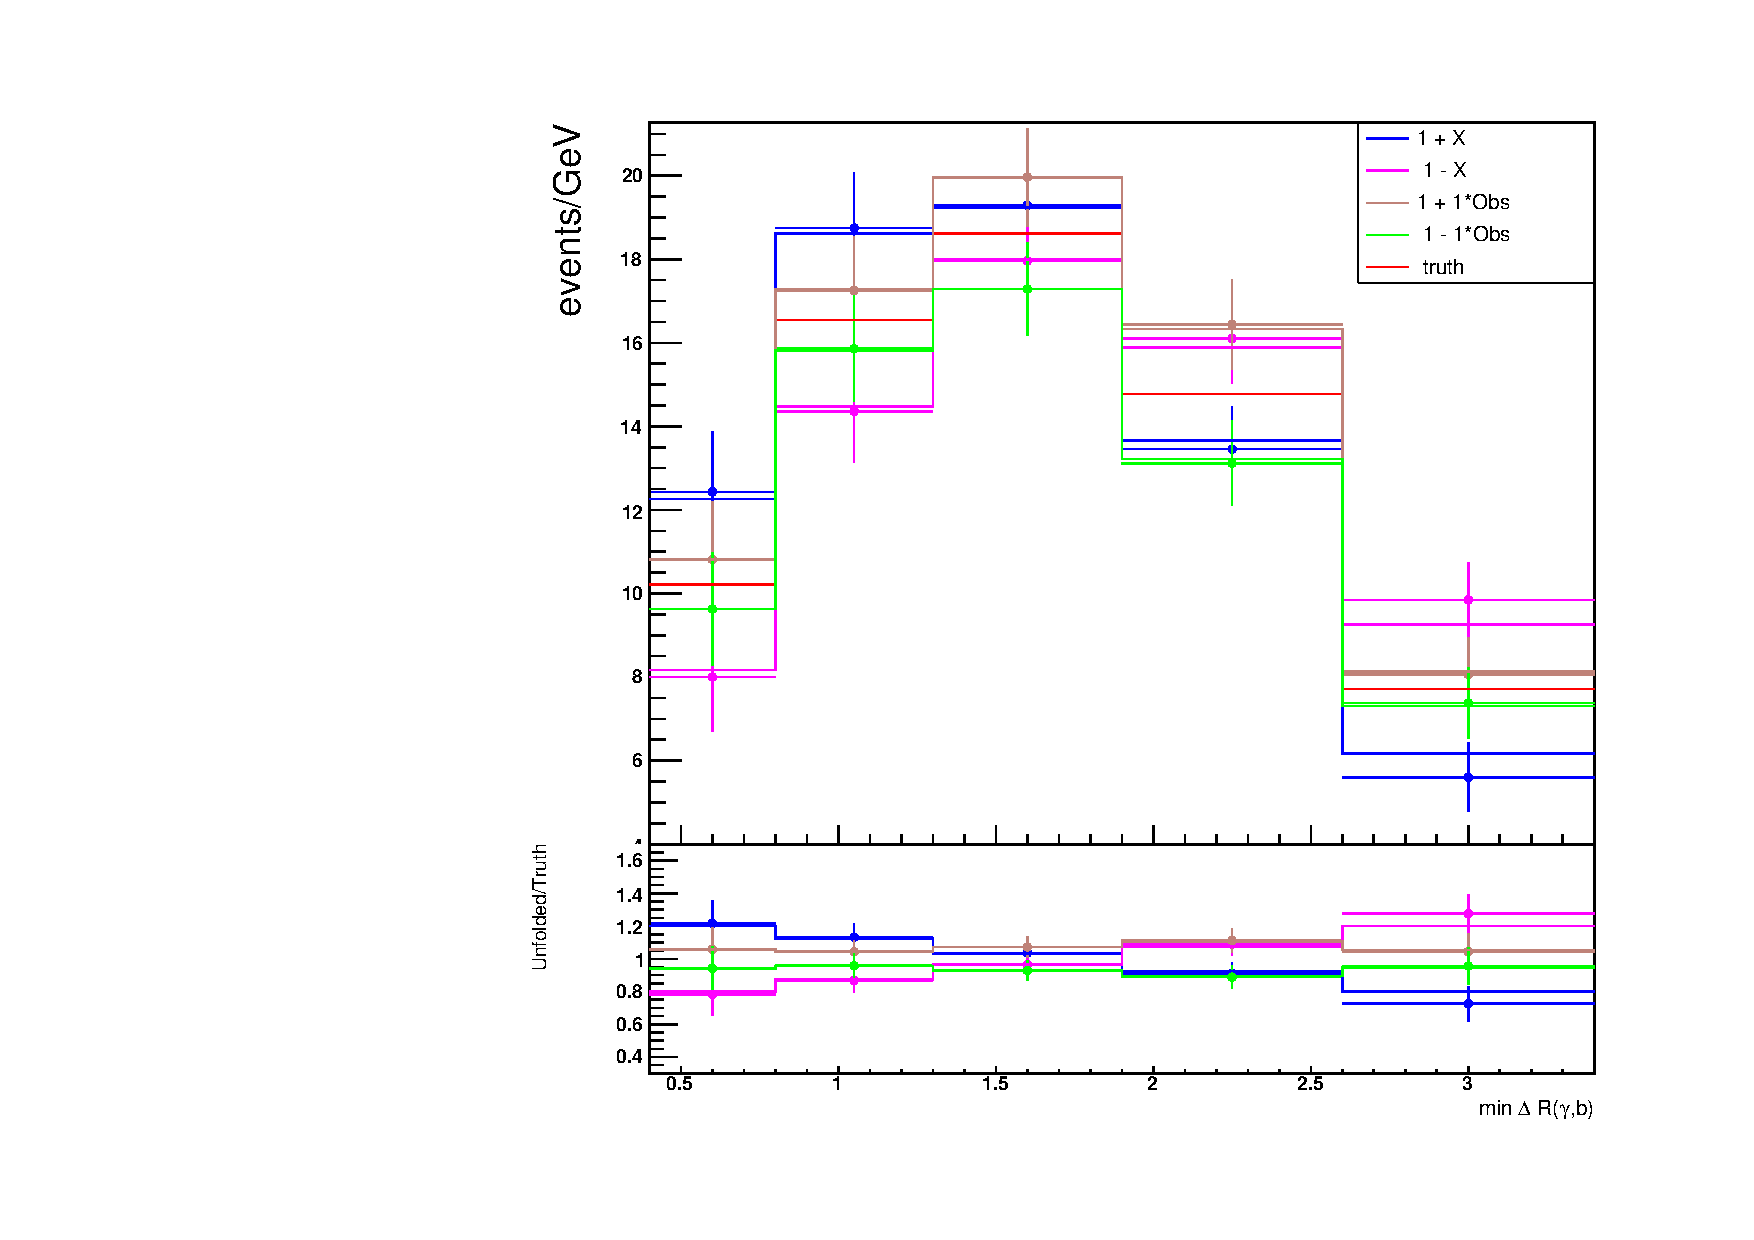
\includegraphics[width=0.4\textwidth]{figures/diff_xsec/dilep/Unfolding_tests/Stress_test/tty2l_drphb_all_stat.pdf}}
  \quad\quad
  \subfloat[]{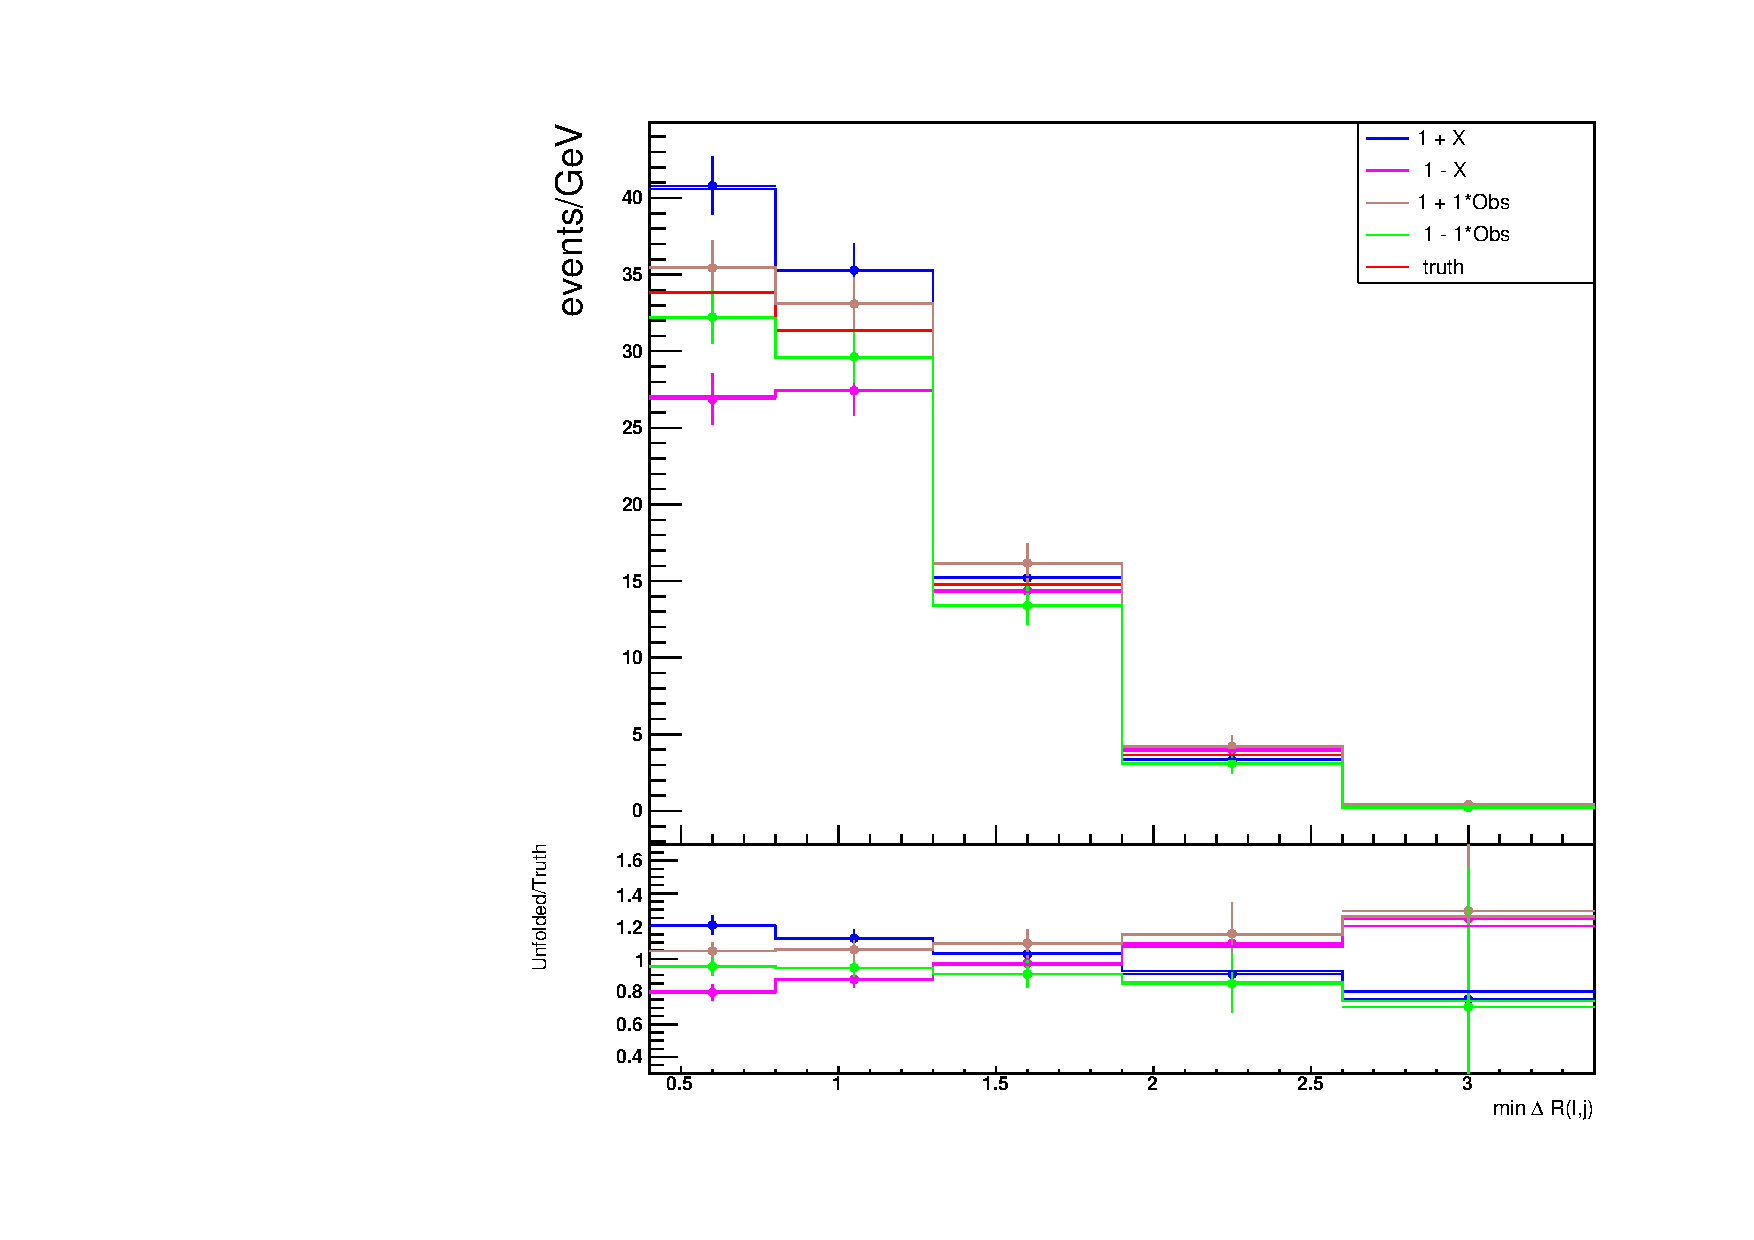
\includegraphics[width=0.4\textwidth]{figures/diff_xsec/dilep/Unfolding_tests/Stress_test/tty2l_drlj_all_stat.pdf}}
  \quad\quad
  \subfloat[]{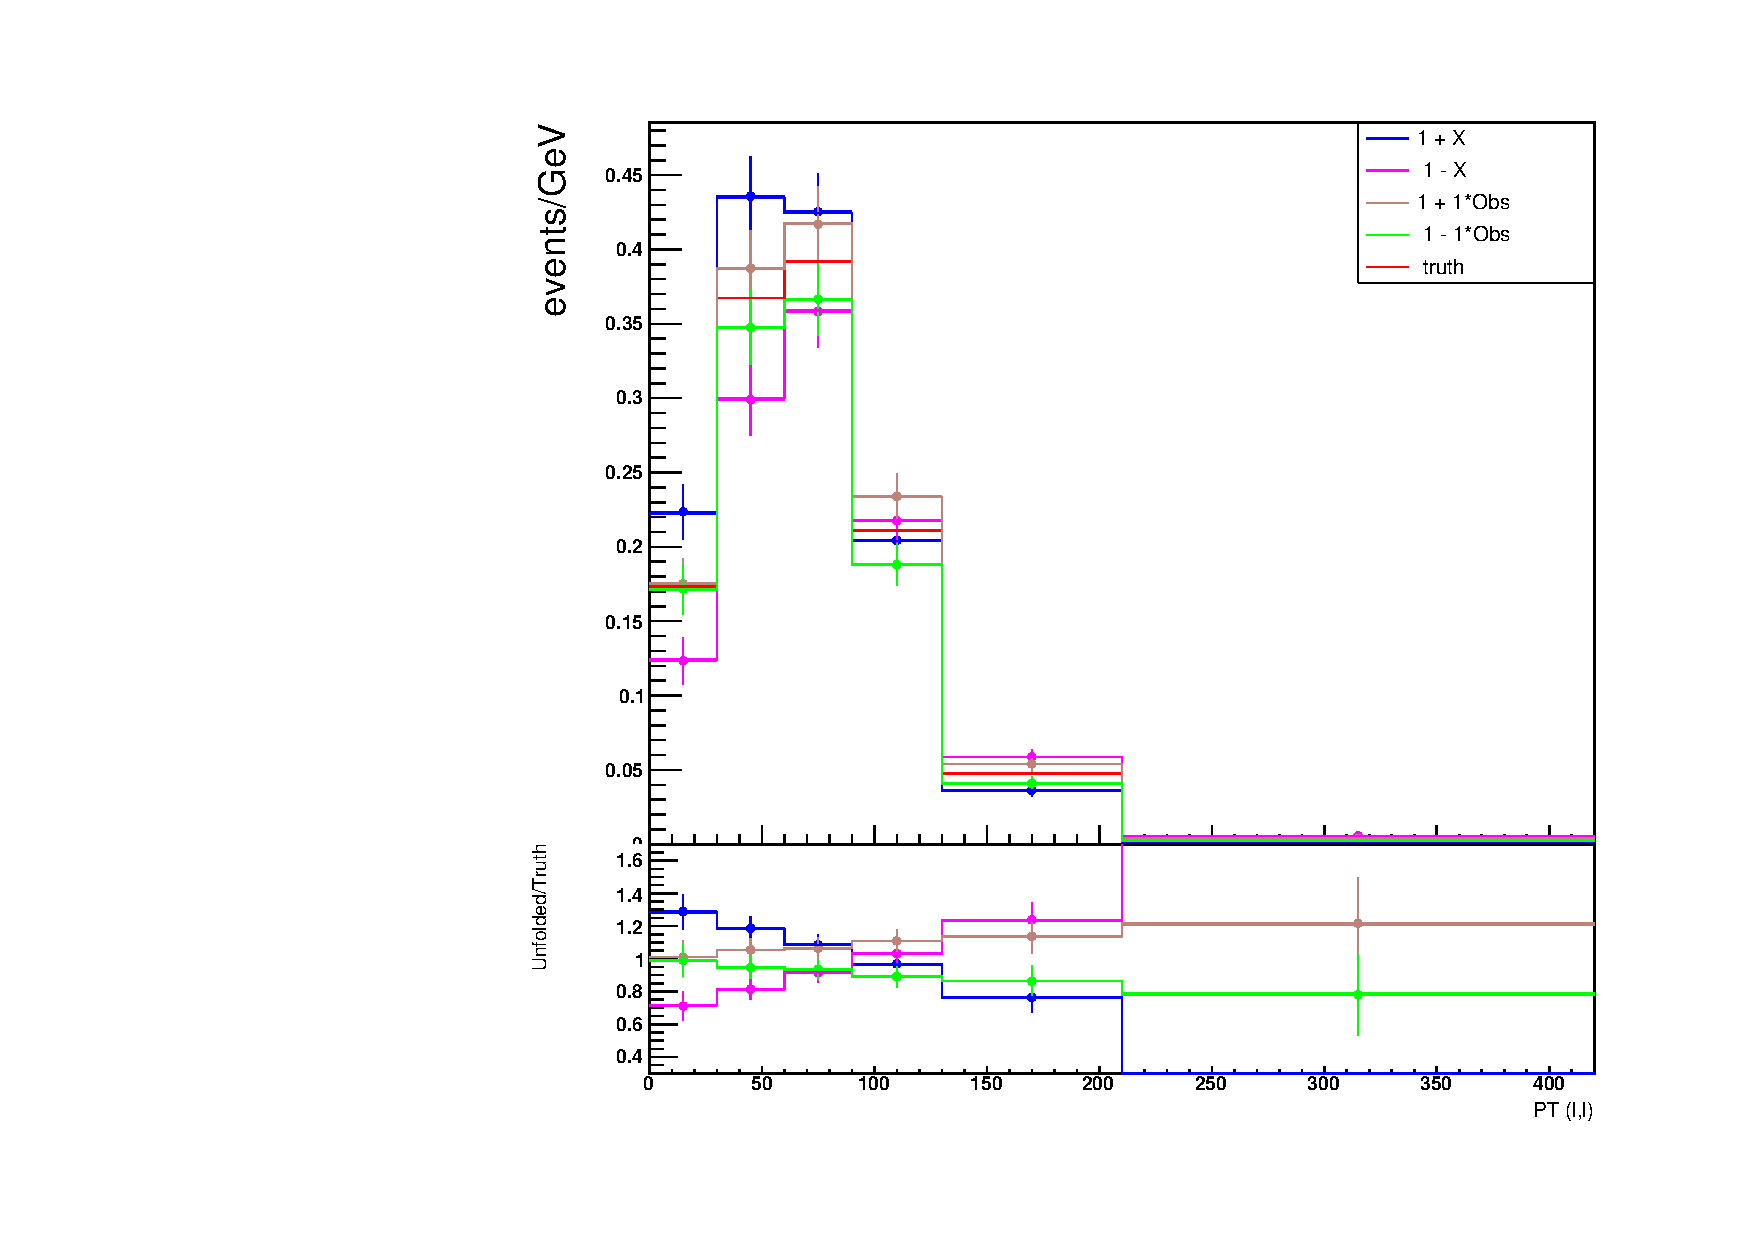
\includegraphics[width=0.4\textwidth]{figures/diff_xsec/dilep/Unfolding_tests/Stress_test/tty2l_ptll_all_stat.pdf}}
  \quad\quad
  \subfloat[]{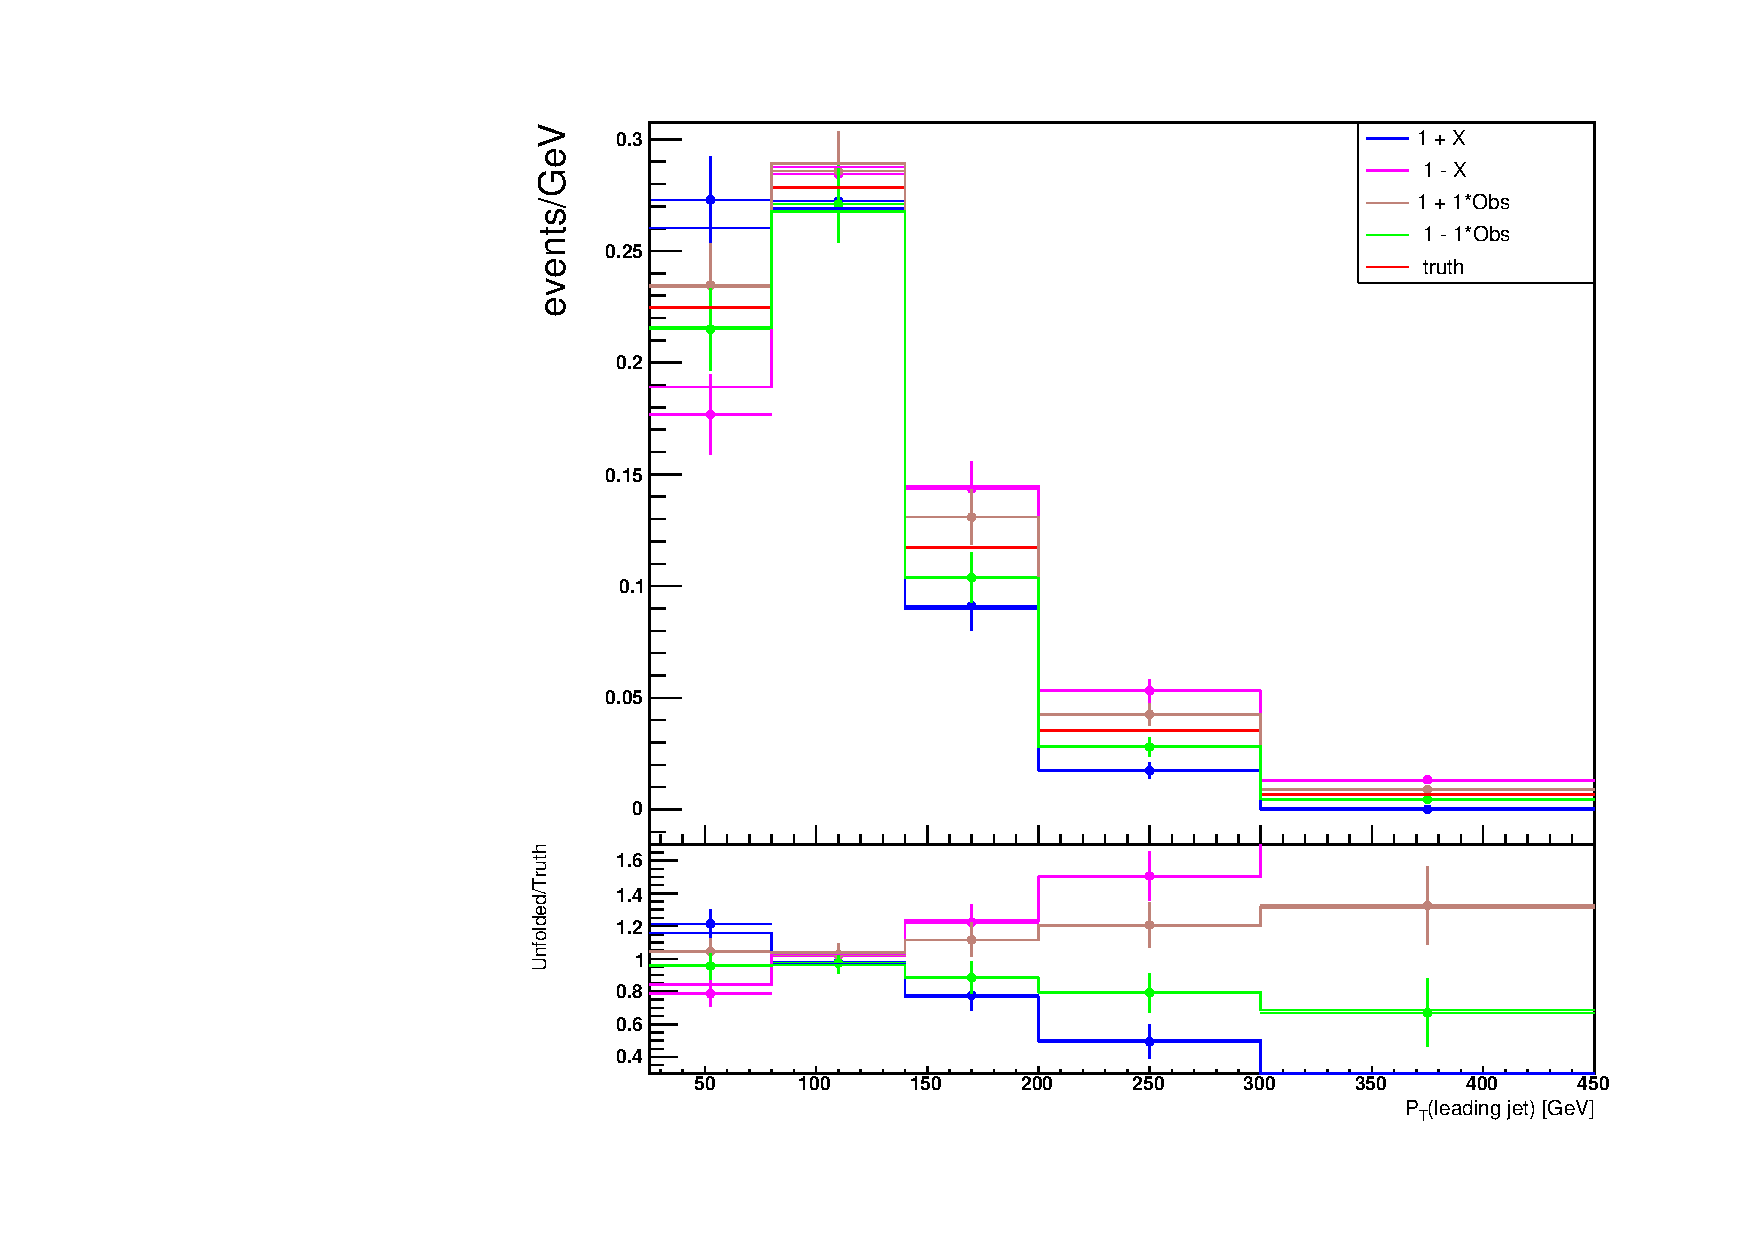
\includegraphics[width=0.4\textwidth]{figures/diff_xsec/dilep/Unfolding_tests/Stress_test/tty2l_ptj1_all_stat.pdf}}
  \quad\quad
  \caption{Stress test for the five observables in the dilepton channel for \tty production measurement. Both the dots and lines are ratios made with respect to the nominal particle level.The dots are the ratio of the unfolded reweighted distributions to the nominal particle level distribution, while the solid lines are the ratio of the reweighted particle level distributions to the nominal one. X is defined in previous section. The uncertainty bars displayed in the plots represent only the statistical error considered in the unfolding.}

  \label{fig:unfolded_dilep_dist_stress_test_2}
\end{figure}
\FloatBarrier

